\documentclass{beamer}

\usepackage[hidelinks]{hyperref}                                            % links
\usepackage{pgfplots}\pgfplotsset{compat=1.18}                              % plots
\usepackage{amsfonts, amsmath, amssymb, amsthm}                             % basic maths commands
\usepackage{mathtools, mathrsfs}                                            % more maths commands
\usepackage{graphicx}                                                       % images and other graphics
\usepackage{geometry}                                                       % page layout
\usepackage{tikz, tikz-3dplot, tikzpagenodes}                               % maths figures
\usepackage{caption, subcaption}                                            % captions outside float
\usepackage{xcolor}                                                         % more colors
\usepackage{enumitem}                                                       % enumerate and itemize indents
\usepackage{nicematrix}                                                     % matrices and tables

\usetikzlibrary{matrix, positioning, patterns, decorations.markings, arrows, arrows.meta, backgrounds, math, cd}

\hypersetup{colorlinks=true, allcolors=magenta}
\definecolor{darkGreen}{HTML}{00A000}
\newgeometry{margin = 1in}

\newtheorem{theorem}{Theorem}[section]
\newtheorem{mainTheorem}{Theorem}
\newtheorem{proposition}[theorem]{Proposition}
\newtheorem{lemma}[theorem]{Lemma}
\newtheorem{corollary}[theorem]{Corollary}
\theoremstyle{definition}\newtheorem{example}[theorem]{Example}
\theoremstyle{definition}\newtheorem{definition}[theorem]{Definition}
\theoremstyle{definition}\newtheorem{remark}[theorem]{Remark}
\theoremstyle{definition}\newtheorem{notation}[theorem]{Notation}
\renewcommand{\themainTheorem}{\Alph{mainTheorem}}
\newtheorem*{theorem*}{Theorem}
\newtheorem*{proposition*}{Proposition}
\newtheorem*{lemma*}{Lemma}
\newtheorem*{corollary*}{Corollary}
\theoremstyle{definition}\newtheorem*{example*}{Example}
\theoremstyle{definition}\newtheorem*{definition*}{Definition}
\theoremstyle{definition}\newtheorem*{remark*}{Remark}
\theoremstyle{definition}\newtheorem*{notation*}{Notation}

% Operators
    \newcommand{\id}{\operatorname{id}}
    \newcommand{\im}{\operatorname{im}}
    \newcommand{\rk}{\operatorname{rk}}
    \newcommand{\ch}{\operatorname{ch}}
    \newcommand{\tr}{\operatorname{tr}}
    \newcommand{\tp}{\operatorname{tp}}
    \newcommand{\qd}{\operatorname{qd}}
    \newcommand{\ON}{\operatorname{ON}}
    \newcommand{\GL}{\operatorname{GL}}
    \newcommand{\SL}{\operatorname{SL}}
    \newcommand{\Id}{\operatorname{Id}}
    \newcommand{\Th}{\operatorname{Th}}
    \newcommand{\Cn}{\operatorname{Cn}}
    \newcommand{\Bl}{\operatorname{Bl}}
    \newcommand{\Cl}{\operatorname{Cl}}
    \newcommand{\LT}{\operatorname{LT}}
    \newcommand{\dom}{\operatorname{dom}}
    \newcommand{\ran}{\operatorname{ran}}
    \newcommand{\cdm}{\operatorname{cdm}}
    \newcommand{\sgn}{\operatorname{sgn}}
    \newcommand{\lcm}{\operatorname{lcm}}
    \newcommand{\ord}{\operatorname{ord}}
    \newcommand{\cvx}{\operatorname{cvx}}
    \newcommand{\Aut}{\operatorname{Aut}}
    \newcommand{\Inn}{\operatorname{Inn}}
    \newcommand{\Out}{\operatorname{Out}}
    \newcommand{\End}{\operatorname{End}}
    \newcommand{\Mat}{\operatorname{Mat}}
    \newcommand{\Obj}{\operatorname{Obj}}
    \newcommand{\Hom}{\operatorname{Hom}}
    \newcommand{\Tor}{\operatorname{Tor}}
    \newcommand{\Ann}{\operatorname{Ann}}
    \newcommand{\Sym}{\operatorname{Sym}}
    \newcommand{\Cov}{\operatorname{Cov}}
    \newcommand{\Orb}{\operatorname{Orb}}
    \newcommand{\Sat}{\operatorname{Sat}}
    \newcommand{\Thm}{\operatorname{Thm}}
    \newcommand{\Der}{\operatorname{Der}}
    \newcommand{\Age}{\operatorname{Age}}
    \newcommand{\Div}{\operatorname{Div}}
    \newcommand{\PGL}{\operatorname{PGL}}
    \newcommand{\rank}{\operatorname{rank}}
    \newcommand{\proj}{\operatorname{proj}}
    \newcommand{\diag}{\operatorname{diag}}
    \newcommand{\eval}{\operatorname{eval}}
    \newcommand{\cont}{\operatorname{cont}}
    \newcommand{\diam}{\operatorname{diam}}
    \newcommand{\mult}{\operatorname{mult}}
    \newcommand{\Core}{\operatorname{Core}}
    \newcommand{\Term}{\operatorname{Term}}
    \newcommand{\Taut}{\operatorname{Taut}}
    \newcommand{\Sent}{\operatorname{Sent}}
    \newcommand{\Skew}{\operatorname{Skew}}
    \newcommand{\Frac}{\operatorname{Frac}}
    \newcommand{\Stab}{\operatorname{Stab}}
    \newcommand{\Isom}{\operatorname{Isom}}
    \newcommand{\Meas}{\operatorname{Meas}}
    \newcommand{\Diag}{\operatorname{Diag}}
    \newcommand{\Sing}{\operatorname{Sing}}
    \newcommand{\coker}{\operatorname{coker}}
    \newcommand{\preim}{\operatorname{preim}}
    \newcommand{\Graph}{\operatorname{Graph}}
    \newcommand{\UnSat}{\operatorname{UnSat}}
    \newcommand{\Axioms}{\operatorname{Axioms}}
    \renewcommand{\Re}{\operatorname{Re}}
    \renewcommand{\Im}{\operatorname{Im}}
    \renewcommand{\div}{\operatorname{div}}
    \renewcommand{\span}{\operatorname{span}}
    \renewcommand{\Form}{\operatorname{Form}}

% Math notations
    % Set Theory, Category Theory, and Logic
        \newcommand{\fa}{\forall}
        \newcommand{\ex}{\exists}
        \newcommand{\MP}{\textrm{MP}}
        \newcommand{\PA}{\textrm{PA}}
        \newcommand{\PL}{{\rm P{\small L}}}
        \newcommand{\DLO}{\textrm{DLO}}
        \newcommand{\ZFC}{\textrm{ZFC}}
        \newcommand{\ACF}{\textrm{ACF}}
        \newcommand{\FOL}{{\rm F{\small OL}}}
        \newcommand{\iso}{\cong}
        \newcommand{\pow}{\mathcal{P}}
        \newcommand{\comp}{\setminus}
        \newcommand{\into}{\hookrightarrow}
        \newcommand{\onto}{\twoheadrightarrow}
        \newcommand{\parto}{\rightharpoonup}
        \newcommand{\eqnum}{\approx}
        \newcommand{\natiso}{\simeq}
        \newcommand{\proves}{\vdash}
        \newcommand{\adjoin}{^\smallfrown}
        \newcommand{\nproves}{\nvdash}
        \newcommand{\symdiff}{\vartriangle}
        \newcommand{\infrule}{\rightsquigarrow}
        \newcommand{\eleminto}{\into_e}
        \newcommand{\elemequiv}{\equiv}
        \newcommand{\substruct}{<}
        \newcommand{\supstruct}{>}
        \newcommand{\elemembed}{\preceq}
        \newcommand{\elemextend}{\succeq}
        \newcommand{\substructeq}{\leq}
        \newcommand{\supstructeq}{\geq}
        \renewcommand{\em}{\varnothing}
        \renewcommand{\vec}[1]{\bar{#1}}

    % Complexity Theory
        \newcommand{\NP}{\mathsf{NP}}
        \newcommand{\coNP}{\mathsf{coNP}}

    % Categories
        \newcommand{\cat}[1]{\textbf{#1}}
        \newcommand{\catset}{\cat{Set}}
        \newcommand{\catgrp}{\cat{Grp}}
        \newcommand{\catmon}{\cat{Mon}}
        \newcommand{\cattop}{\cat{Top}}
        \newcommand{\catmet}{\cat{Met}}
        \newcommand{\catrel}{\cat{Rel}}
        \newcommand{\catord}{\cat{Ord}}
        \newcommand{\catscat}{\cat{Cat}}
        \newcommand{\catlscat}{\cat{CAT}}
        \newcommand{\catgrpd}{\cat{Grpd}}
        \newcommand{\catring}{\cat{Ring}}
        \newcommand{\cathtop}{\cat{hTop}}
        \newcommand{\catptop}{\cat{Top}_\blob}
        \newcommand{\catphtop}{\cat{hTop}_\blob}
        \newcommand{\catabgrp}{\cat{Ab}}
        \newcommand{\catman}[1][\infty]{\cat{Man}_{#1}}
        \newcommand{\cathom}[1][\mc{L}]{#1\textrm{-}\cat{Hom}}
        \newcommand{\catemb}[1][\mc{L}]{#1\textrm{-}\cat{Emb}}
        \newcommand{\catmod}[1][R]{\prescript{}{#1}{\cat{Mod}}}
        \newcommand{\catrmod}[1][R]{\cat{Mod}_{#1}}
        \newcommand{\catcov}[1][X]{\cat{Cov}\l(#1\r)}
        \newcommand{\catfgmod}[1][R]{\cat{fg}_{#1}\cat{Mod}}
        \newcommand{\catvect}[1][k]{\prescript{}{#1}{\cat{Vect}}}
        \newcommand{\catfgvect}[1][k]{\cat{fg}_{#1}\cat{Vect}}
        \newcommand{\catalg}[1][R]{\prescript{}{#1}{\cat{Alg}}}
        \newcommand{\catgset}[1]{\prescript{}{#1}{\cat{Set}}}
        \newcommand{\catmodel}[2][\mc{L}]{\mc{M}_#1\!\l(#2\r)}
        \newcommand{\catrep}[2][\,]{\cat{Rep}_{#1\!}\l(#2\r)}
        \newcommand{\catfgrep}[2][\,]{\cat{fgRep}_{#1\!}\l(#2\r)}

    % Analysis
        \newcommand{\BV}{BV}
        \newcommand{\del}{\partial}
        \newcommand{\incto}{\nearrow}
        \newcommand{\decto}{\searrow}
        \newcommand{\abscont}{\ll}
        \newcommand{\esssup}{\operatorname{ess-sup}}
        \renewcommand{\d}{\mathrm{d}}

    % Topology
        \newcommand{\rel}{\,\operatorname{rel}\,}
        \newcommand{\tcl}{\operatorname{cl}}
        \newcommand{\scl}{\operatorname{scl}}
        \newcommand{\tint}{\operatorname{int}}
        \newcommand{\sint}{\operatorname{sint}}
        \newcommand{\htopeq}{\simeq}
        \newcommand{\pathto}{\rightsquigarrow}

    % Linear Algebra
        \newcommand{\dual}{\wedge}
        \newcommand{\adj}{\ast}
        \newcommand{\trans}{\mathsf{T}}
        \newcommand{\inprod}[2]{\l\langle{#1},{#2}\r\rangle}

    % Group Theory
        \newcommand{\act}{\curvearrowright}
        \newcommand{\semi}{\rtimes}
        \newcommand{\nsubgrp}{\triangleleft}
        \newcommand{\nsupgrp}{\triangleright}
        \newcommand{\nsubgrpeq}{\trianglelefteq}
        \newcommand{\nsupgrpeq}{\trianglerighteq}

    % Number Theory
        \newcommand{\divides}{\,|\,}
        \newcommand{\ndivides}{\nmid}
        \renewcommand{\mod}[1]{\l(\operatorname{mod}\,#1\r)}

    % Algebraic Geometry
        \newcommand{\ratto}{\dashrightarrow}

    % Misc
        \newcommand{\st}{:}
        \newcommand{\tpl}[1]{\l(#1\r)}
        \newcommand{\gen}[1]{\l\langle#1\r\rangle}
        \renewcommand{\bar}{\overline}

% Math others
    % Number Systems
        \newcommand{\N}{\mathbb{N}}
        \newcommand{\Z}{\mathbb{Z}}
        \newcommand{\Q}{\mathbb{Q}}
        \newcommand{\R}{\mathbb{R}}
        \newcommand{\C}{\mathbb{C}}
        \newcommand{\F}{\mathbb{F}}
        \newcommand{\E}{\mathbb{E}}
        \newcommand{\A}{\mathbb{A}}
        \renewcommand{\S}{\mathbb{S}}
        \renewcommand{\P}{\mathbb{P}}
        \renewcommand{\H}{\mathbb{H}}

% LaTeX/MathJax
    % Fonts
        \newcommand{\mc}[1]{\mathcal{#1}}
        \newcommand{\ms}[1]{\mathscr{#1}}
        \newcommand{\mb}[1]{\mathbb{#1}}
        \newcommand{\mf}[1]{\mathfrak{#1}}
        \renewcommand{\it}[1]{\textit{#1}}
        \renewcommand{\bf}[1]{\textbf{#1}}
        \renewcommand{\sf}[1]{\textsf{#1}}
        \renewcommand{\phi}{\varphi}
        \renewcommand{\epsilon}{\varepsilon}

    % Meta
        \newcommand{\blob}{\bullet}
        \newcommand{\slot}{-}
        \newcommand{\cref}[1]{\tag{$\,#1\,$}}
        \newcommand{\qedin}{\tag*{$\blacksquare$}}
        \newcommand{\exqedin}{\tag*{$\blacklozenge$}}
        \renewcommand{\l}{\left}
        \renewcommand{\r}{\right}
        \renewcommand{\qed}{\phantom\qedhere\hfill$\blacksquare$}
        \renewcommand{\ref}[1]{\l(\,#1\,\r)}


\title{\normalsize{Tree-like graphings of countable Borel equivalence relations}}
\subtitle{\scriptsize{An exposition to\\\textit{Tree-like graphings, wallings, and median graphings of equivalence relations}\\by Ruiyuan Chen, Antoine Poulin, Ran Tao, and Anush Tserunyan}}
\author{\small Zhaoshen Zhai}
\date{\footnotesize October 1, 2024}
\titlegraphic{
\includegraphics[width=0.1\textwidth]{img/mcgill.png}}

\usecolortheme{seahorse}
\usefonttheme{serif}
\useinnertheme{rounded}

\begin{document}\frame{\titlepage}
    \begin{frame}{Countable Borel equivalence relations}
        \begin{definition}
            A \textit{countable Borel equivalence relation (CBER)} on a standard Borel space $X$ is a Borel equivalence relation $E\subseteq X^2$ such that each $E$-class is countable.
        \end{definition}

        \pause
        \vspace{-0.1in}

        \begin{example}
            Any Borel action $\Gamma\act X$ of a countable (discrete) group on a standard Borel space induces its \textit{orbit equivalence relation} $E^X_\Gamma$, which is a CBER.
        \end{example}

        \pause
        \vspace{-0.15in}

        \begin{figure}[h]
            \center
            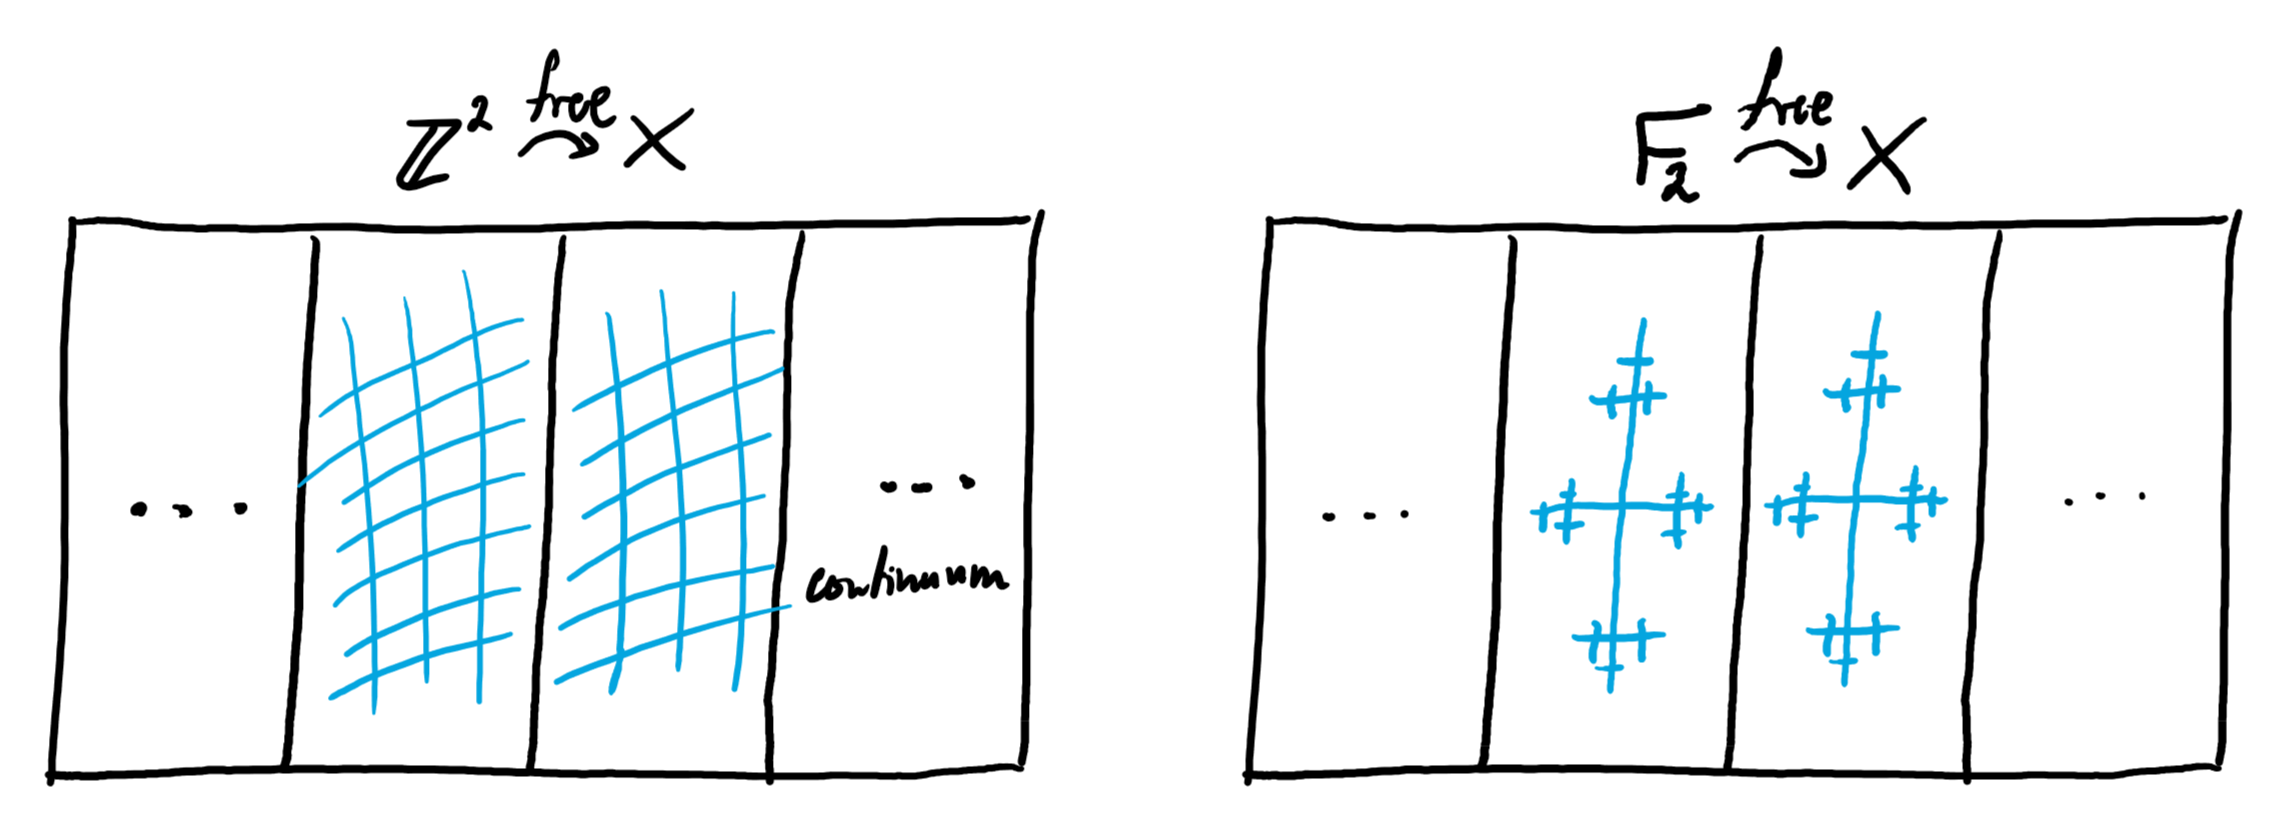
\includegraphics[width=0.9\textwidth]{img/group_action.png}
        \end{figure}
    \end{frame}
    \begin{frame}{Smooth and hyperfinite CBERs}
        \vspace{-0.1in}
        \begin{example}[Smooth]
            \begin{itemize}
                \item[\scriptsize$\blob$] Identity relation on a standard Borel space, say $\R$ or $2^\N$.
                    \pause
                \item[\scriptsize$\blob$] $\Z$-coset equivalence on $\R$: $xE^\R_\Z y$ iff $x-y\in\Z$.
            \end{itemize}
        \end{example}

        \pause
        \vspace{-0.1in}

        \begin{example}[Hyperfinite]
            $E_0$ on $2^\N$, where $xE_0y$ iff $\ex n\in\N,\fa m\geq n:x_m=y_m$.
        \end{example}

        \pause

        This CBER is \textit{hyperfinite}: $E_0=\bigcup_nF_n$ for an increasing sequence $F_0\subseteq F_1\cdots$ of finite Borel equivalence relations:
        \pause
        \vspace{-0.1in}
        \begin{equation*}
            xF_ny\ \ \ \ \leftrightarrow\ \ \ \ \fa m\geq n:x_m=y_m.
        \end{equation*}

        \pause
        \vspace{-0.15in}

        \begin{theorem}[Slaman-Steel, Weiss]
            Let $E$ be a CBER on a standard Borel space $X$. TFAE:
            \begin{itemize}
                \item[$1.$] $E$ is hyperfinite. {\color{gray}\footnotesize $E=\bigcup_nF_n$ where $F_0\subseteq F_1\subseteq\cdots$ are FBERs.}
                \item[$2.$] $E$ is induced by a Borel $\Z$-action. {\color{gray}\footnotesize $E=E_\Z^X$ for some $\Z\act X$.}
            \end{itemize}
        \end{theorem}
    \end{frame}
    \begin{frame}{Smooth and hyperfinite CBERs}
        \vspace{-0.34in}
        \begin{example}[Smooth]
            \begin{itemize}
                \item[\scriptsize$\blob$] Identity relation on a standard Borel space, say $\R$ or $2^\N$.
                \item[\scriptsize$\blob$] $\Z$-coset equivalence on $\R$: $xE^\R_\Z y$ iff $x-y\in\Z$.
            \end{itemize}
        \end{example}

        \vspace{-0.1in}

        \begin{example}[Hyperfinite]
            $E_0$ on $2^\N$, where $xE_0y$ iff $\ex n\in\N,\fa m\geq n:x_m=y_m$.
        \end{example}

        \vspace{-0.15in}

        \begin{figure}[h]
            \center
            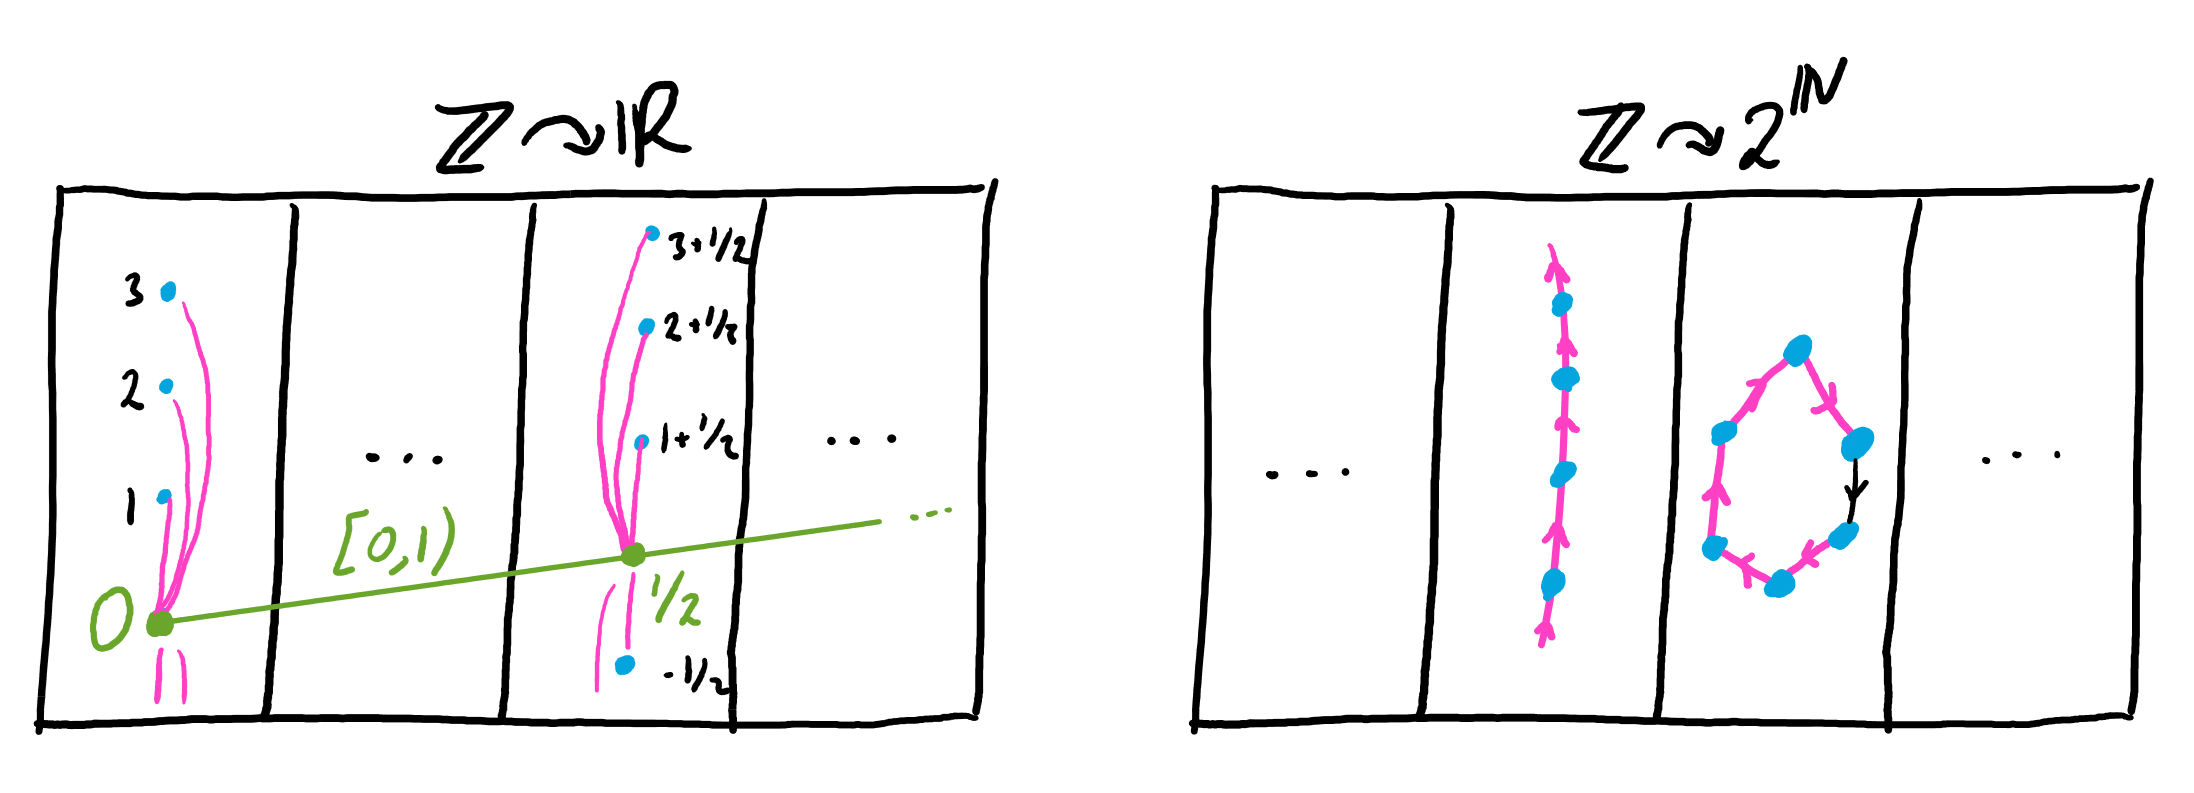
\includegraphics[width=0.9\textwidth]{img/smooth_hyperfinite.png}
        \end{figure}
    \end{frame}
    \begin{frame}{Graphing of a CBER}
        \begin{definition}
            A \textit{graphing} of a CBER $E$ on $X$ is a Borel graph $G\subseteq X^2$ whose connectedness relation is $E$ ($xEy\leftrightarrow xG\cdots Gy$ for all $x,y\in X$).
        \end{definition}

        \pause
        \vspace{-0.15in}

        \begin{figure}[h]
            \center
            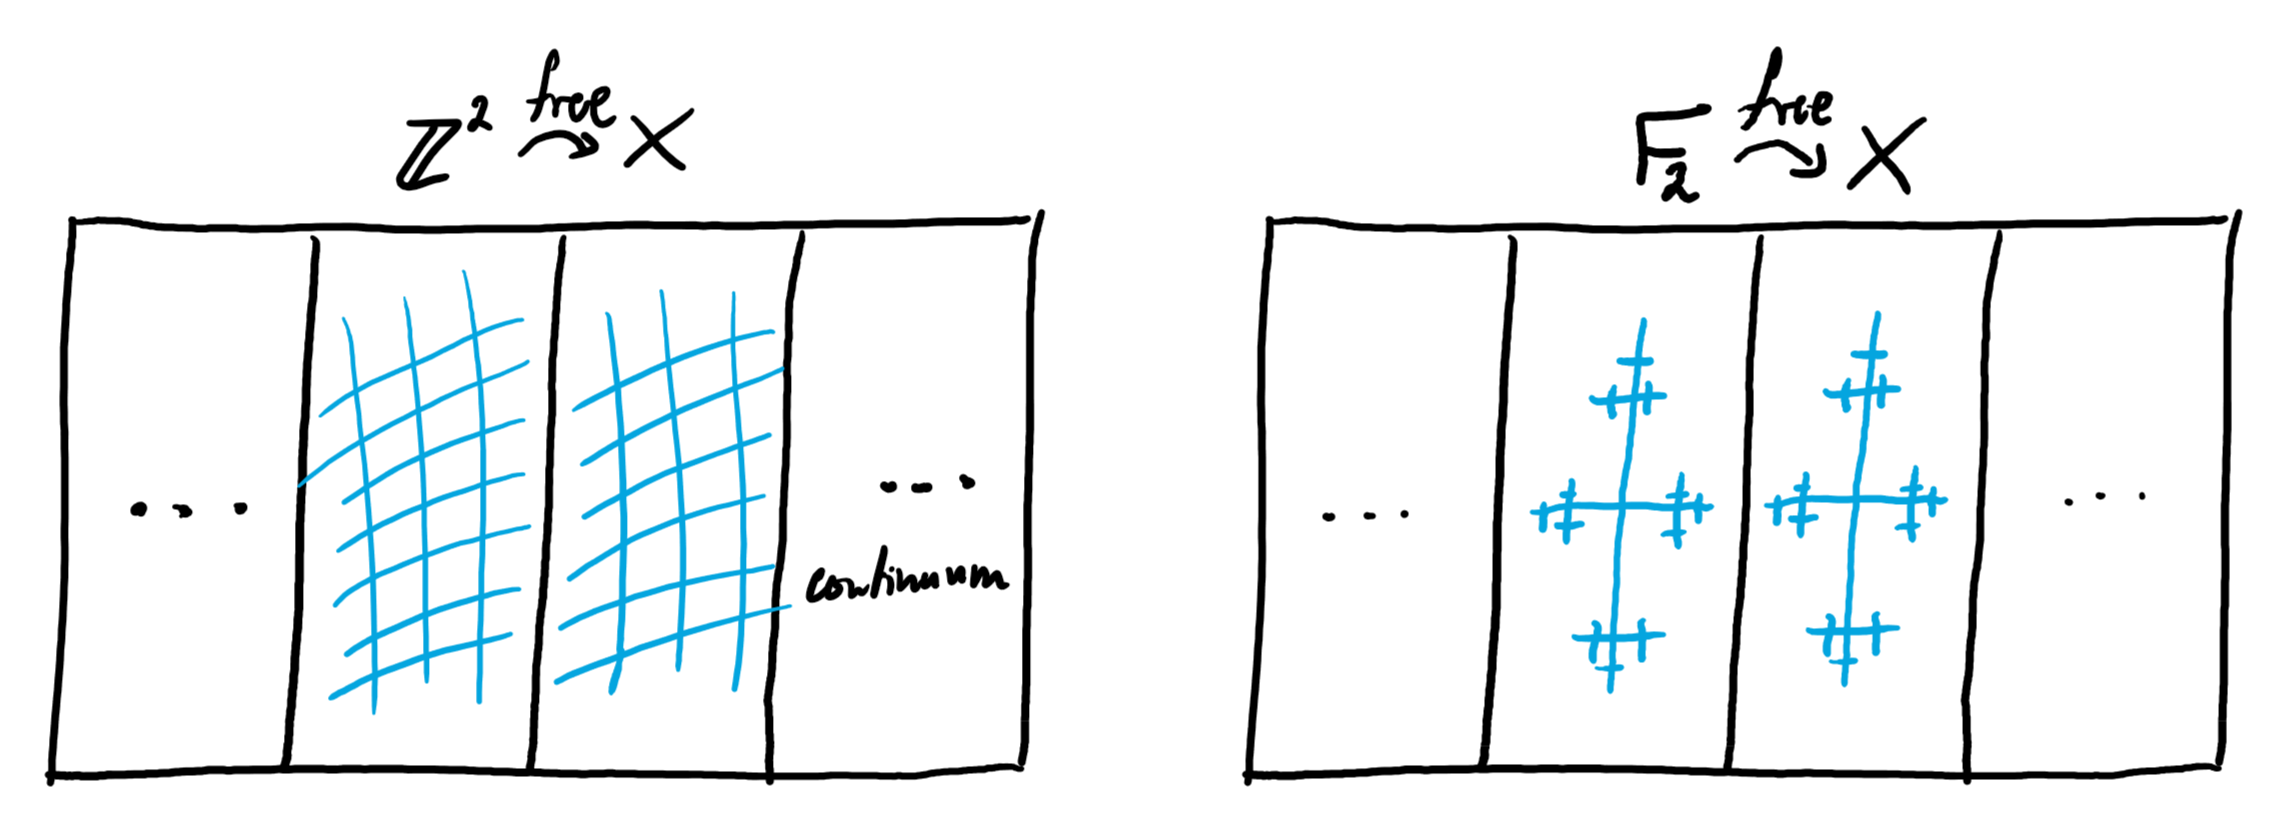
\includegraphics[width=0.7\textwidth]{img/group_action.png}
        \end{figure}
        \vspace{-0.2in}
        \begin{figure}[h]
            \center
            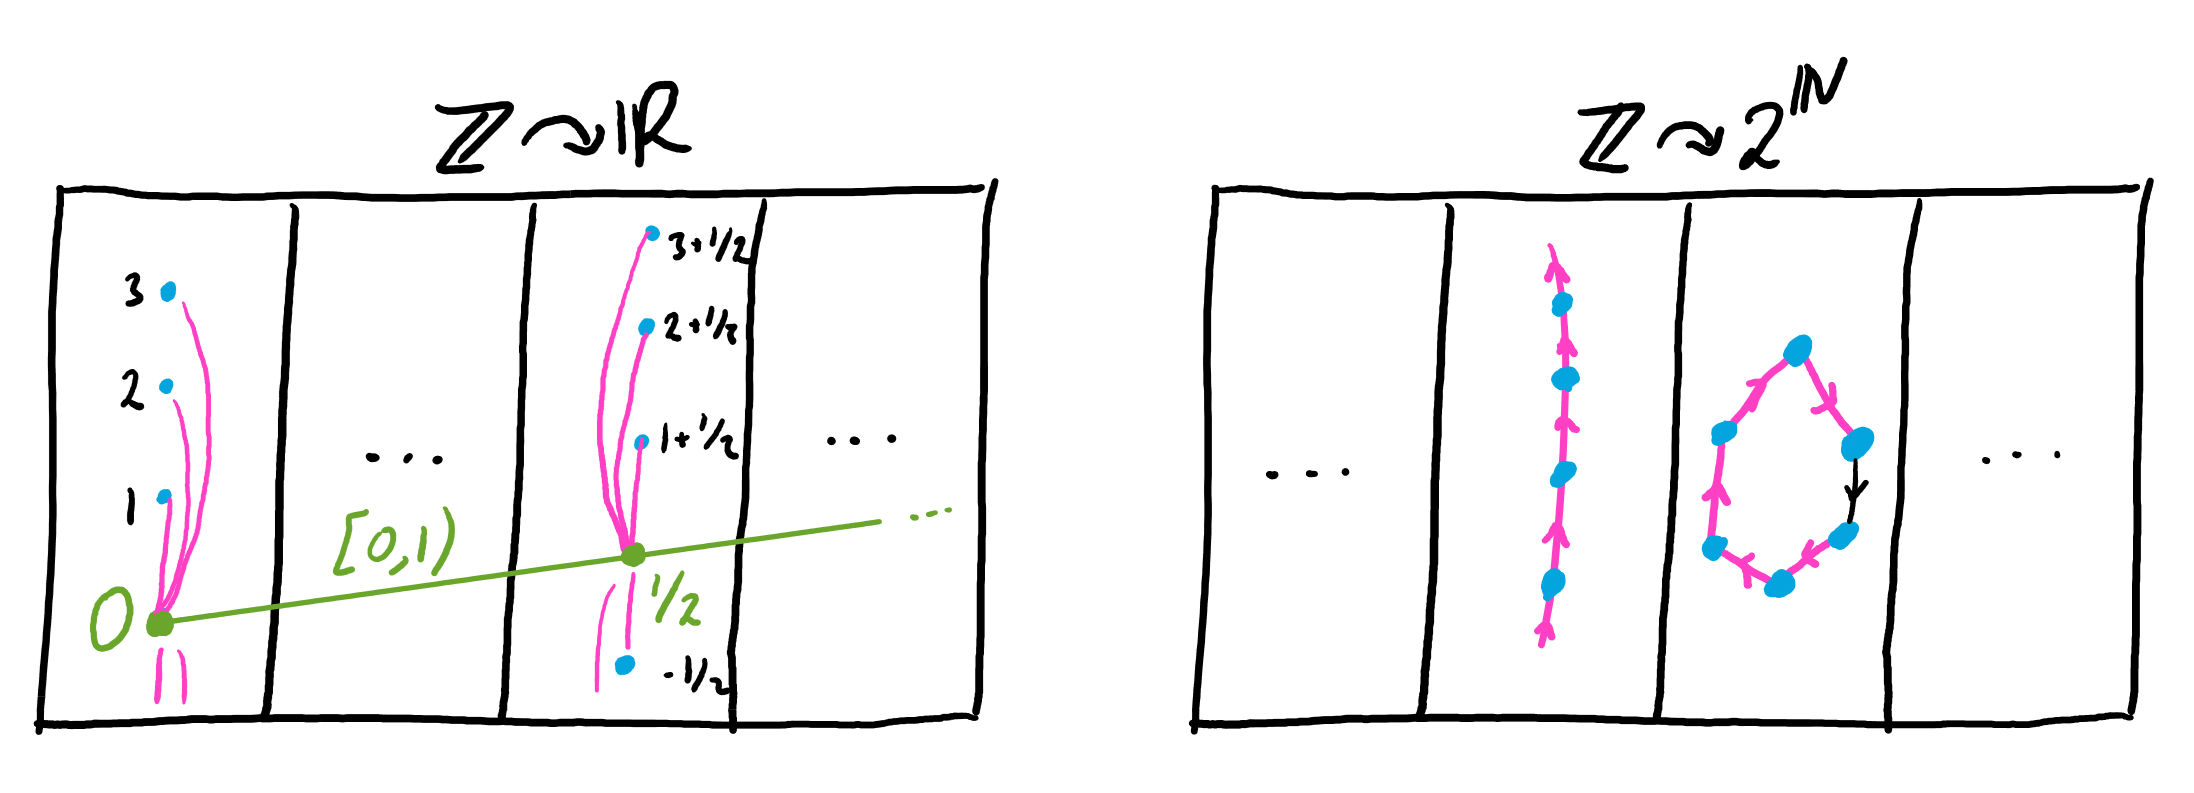
\includegraphics[width=0.7\textwidth]{img/smooth_hyperfinite.png}
        \end{figure}
    \end{frame}
    \begin{frame}{Treeing of a CBER}
        \begin{definition}
            A \textit{treeing} of a CBER $E$ is an acyclic graphing, and a CBER $E$ is said to be \textit{treeable} if it admits a treeing.
        \end{definition}

        \vspace{-0.13in}

        \begin{figure}[h]
            \center
            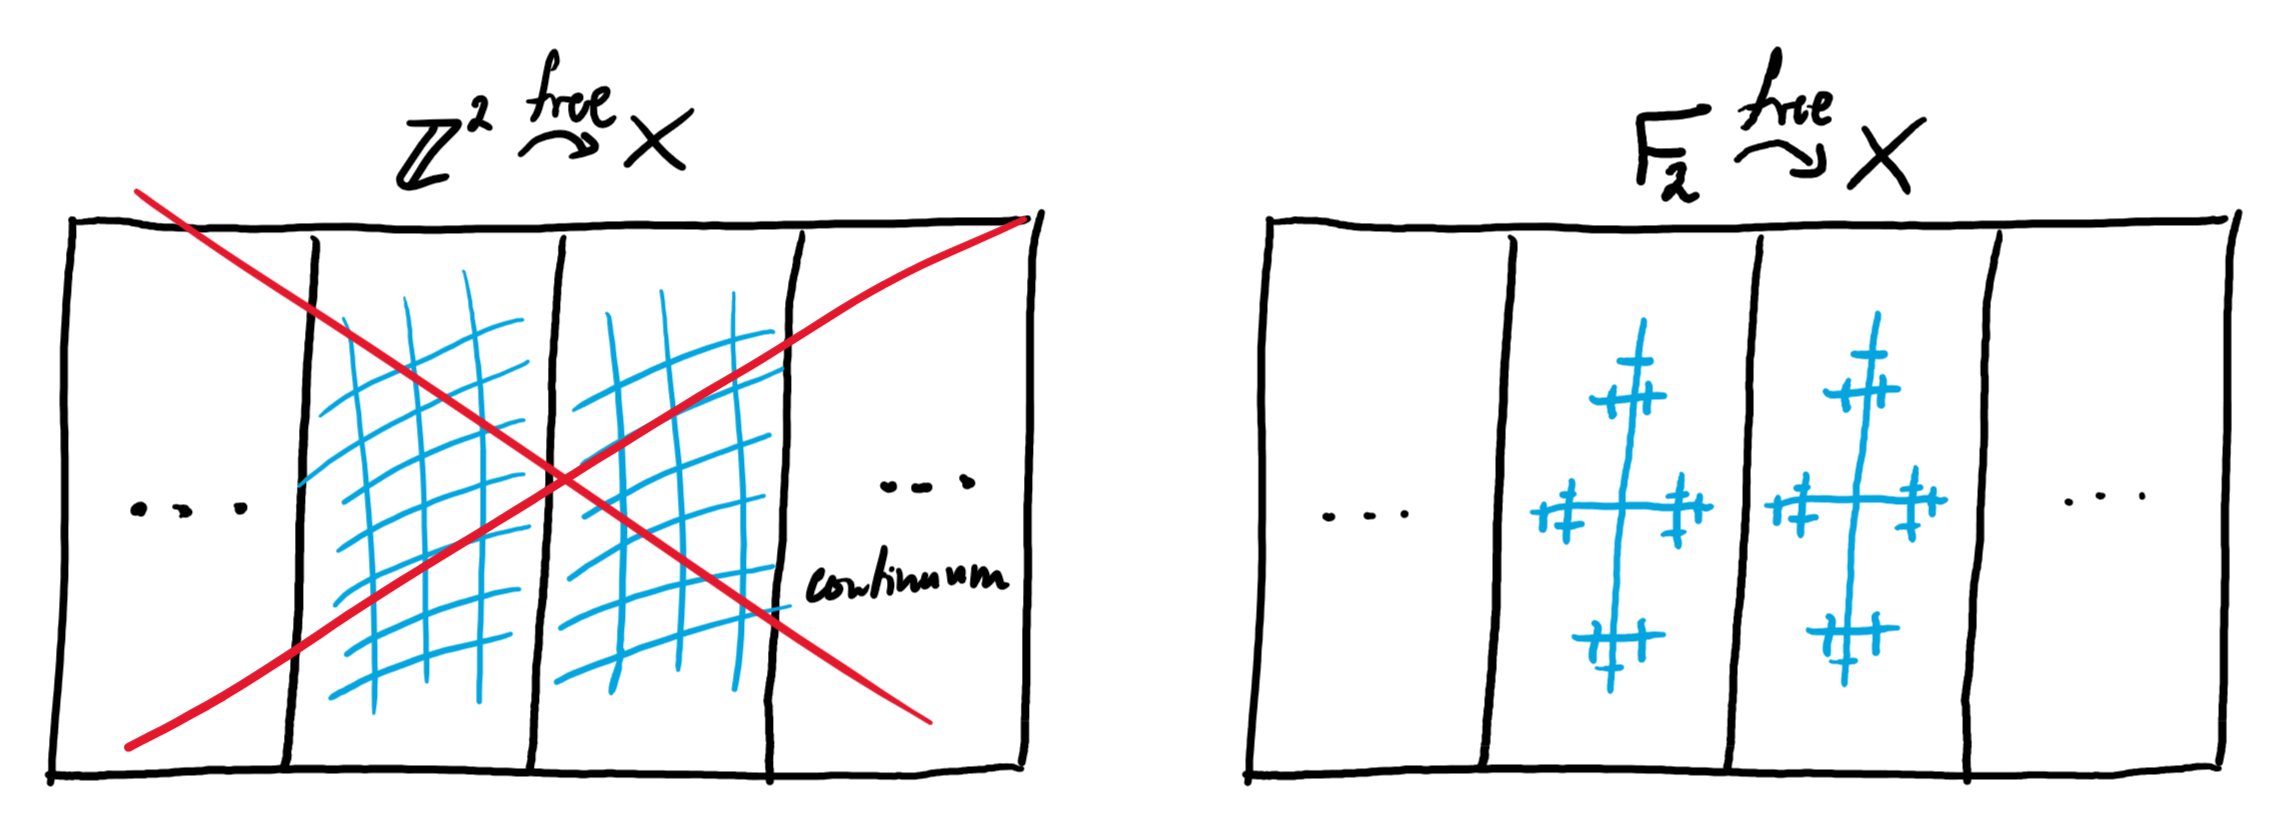
\includegraphics[width=0.7\textwidth]{img/not_treeable.png}
        \end{figure}
        \vspace{-0.2in}
        \begin{figure}[h]
            \center
            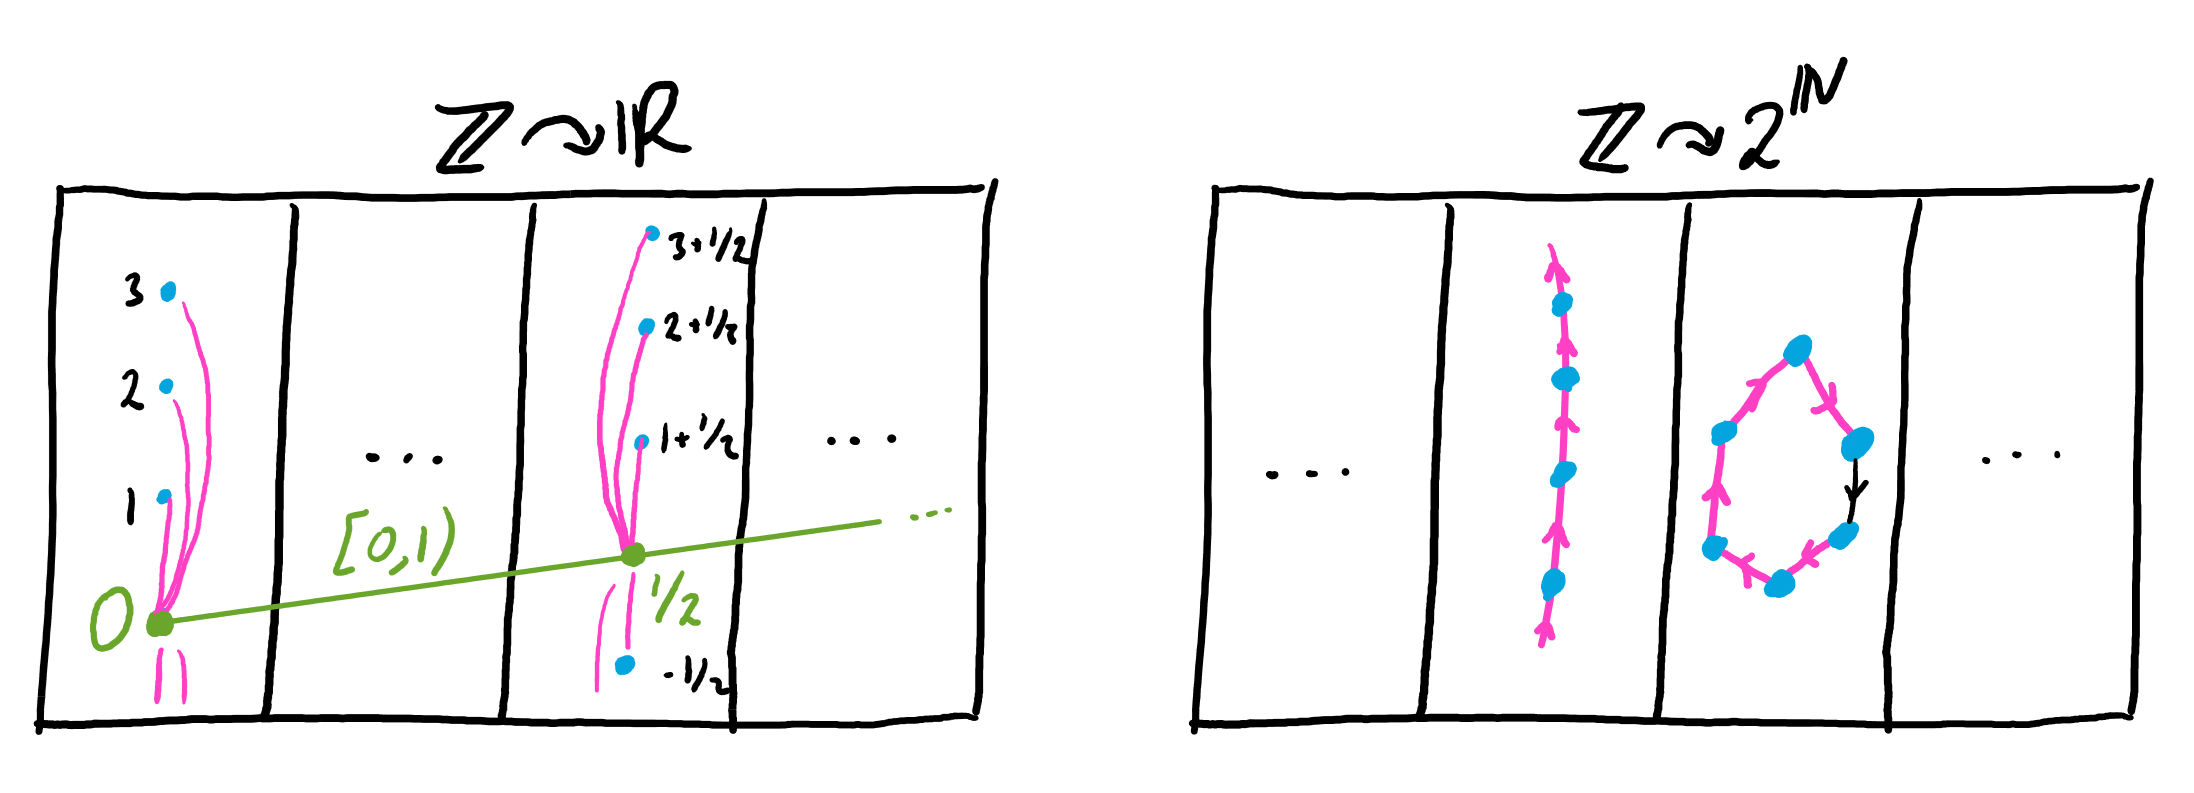
\includegraphics[width=0.7\textwidth]{img/smooth_hyperfinite.png}
        \end{figure}
    \end{frame}
    \begin{frame}{Treeable CBERs}
        \vspace{-0.2in}

        \begin{example}
            Free actions of a free group $F_r\act X$.
        \end{example}

        \begin{figure}[h!]
            \vspace{-0.8in}
            \hfill
            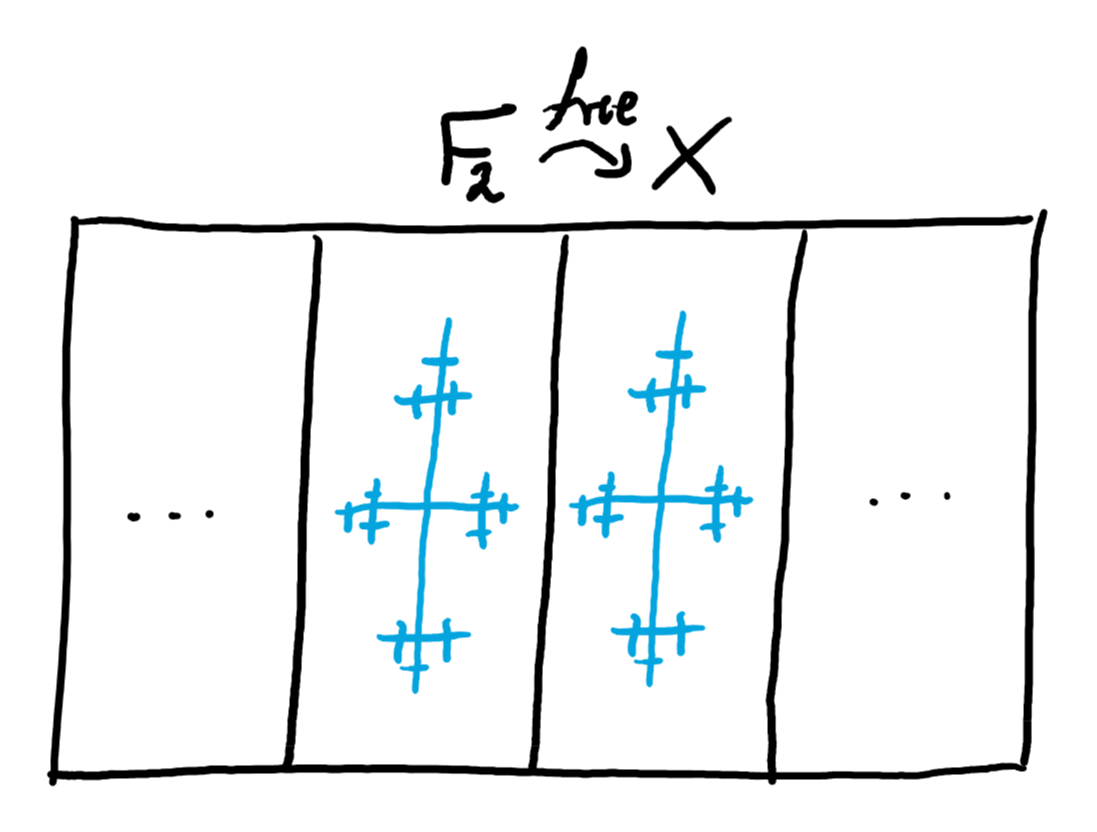
\includegraphics[width=0.3\textwidth]{img/free_group_action.png}
        \end{figure}

        \pause
        \vspace{-0.28in}

        \begin{theorem}[JKL02]
            Free actions of virtually-free groups are treeable.
        \end{theorem}

        \pause

        \begin{theorem}[GdlH90]
            Every finitely-generated group whose Cayley graph is a quasi-tree is virtually-free, and hence treeable.
        \end{theorem}

        \pause

        \begin{question}[Robin Tucker-Drob; 2015]
            Is the class of treeable CBERs robust under quasi-isometries?
        \end{question}
    \end{frame}
    \begin{frame}{Main result}
        \begin{theorem}[Chen, Poulin, Tao, Tserunyan; 2023+]
            If a CBER $E$ admits a locally-finite graphing such that each component is a quasi-tree, then $E$ is treeable.
        \end{theorem}

        \pause
        \vspace{0.1in}

        \scriptsize{
            Two metric spaces $X,Y$ are \textit{quasi-isometric} if they are isometric up to a bounded multiplicative and additive error; $X$ is a \textit{quasi-tree} if it is quasi-isometric to a tree.
            \vspace{-0.3in}
            \begin{figure}[h]
                \center
                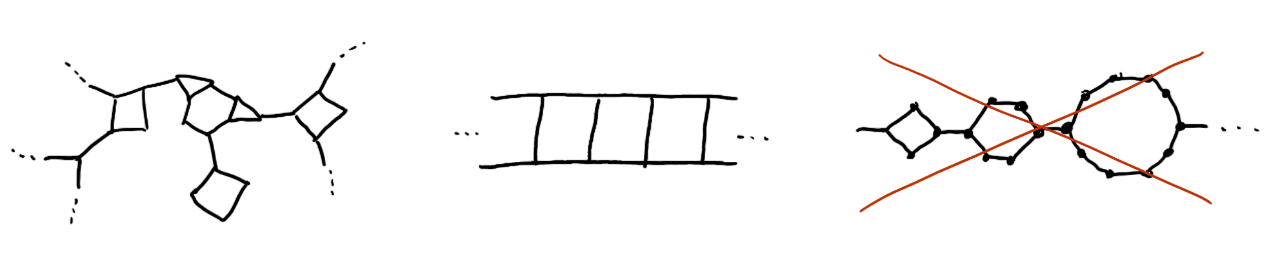
\includegraphics[width=0.9\textwidth]{img/quasi_tree.png}
            \end{figure}
        }
    \end{frame}
    \begin{frame}{Game plan}
        \begin{center}
            \scalebox{0.85}{
                \hspace*{-0.62in}
                \def\hsp{3.75}
                \def\vsp{1.3}
                \def\vsh{0.05}
                \begin{tikzpicture}
                    \draw[dashed, rounded corners, opacity=0.2] (-1.7,0.5) -- (-1.7,-0.4-\vsp) -- (0.75,-0.4-\vsp) -- (3,-0.4) -- (3*\hsp+1.5,-0.4) -- (3*\hsp+1.5,0.5) -- cycle;
                    \draw[dashed, rounded corners, opacity=0.2] (2.5,0.55-\vsp) rectangle (3*\hsp+1.5,-0.45-\vsp);

                    \draw (0,\vsh) circle (0in) node{Quasi-treeing};
                    \draw (3*\hsp,\vsh) circle (0in) node{Treeing};

                    \pause

                    \only<2>{\node[inner sep=0pt] at (5,-5) {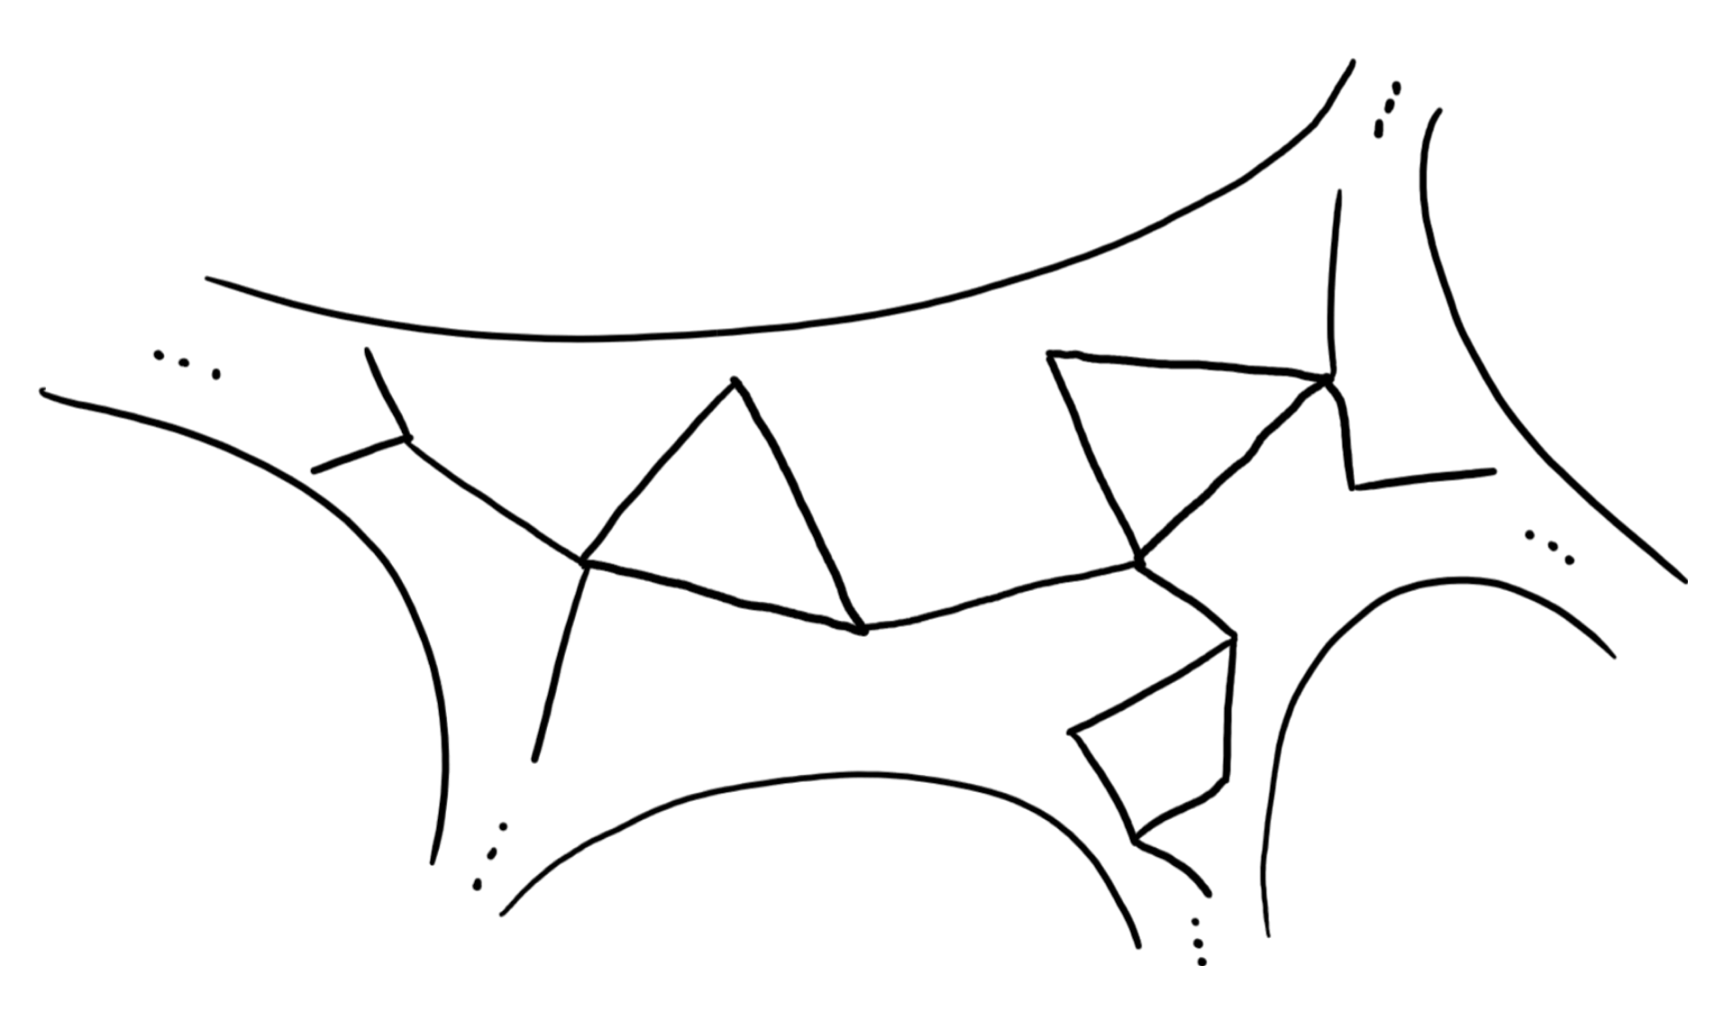
\includegraphics[width=0.9\textwidth]{img/plan/0_base.png}};}
                    \onslide<3,4>{{\transparent{0.5}\node[inner sep=0pt] at (5,-5) {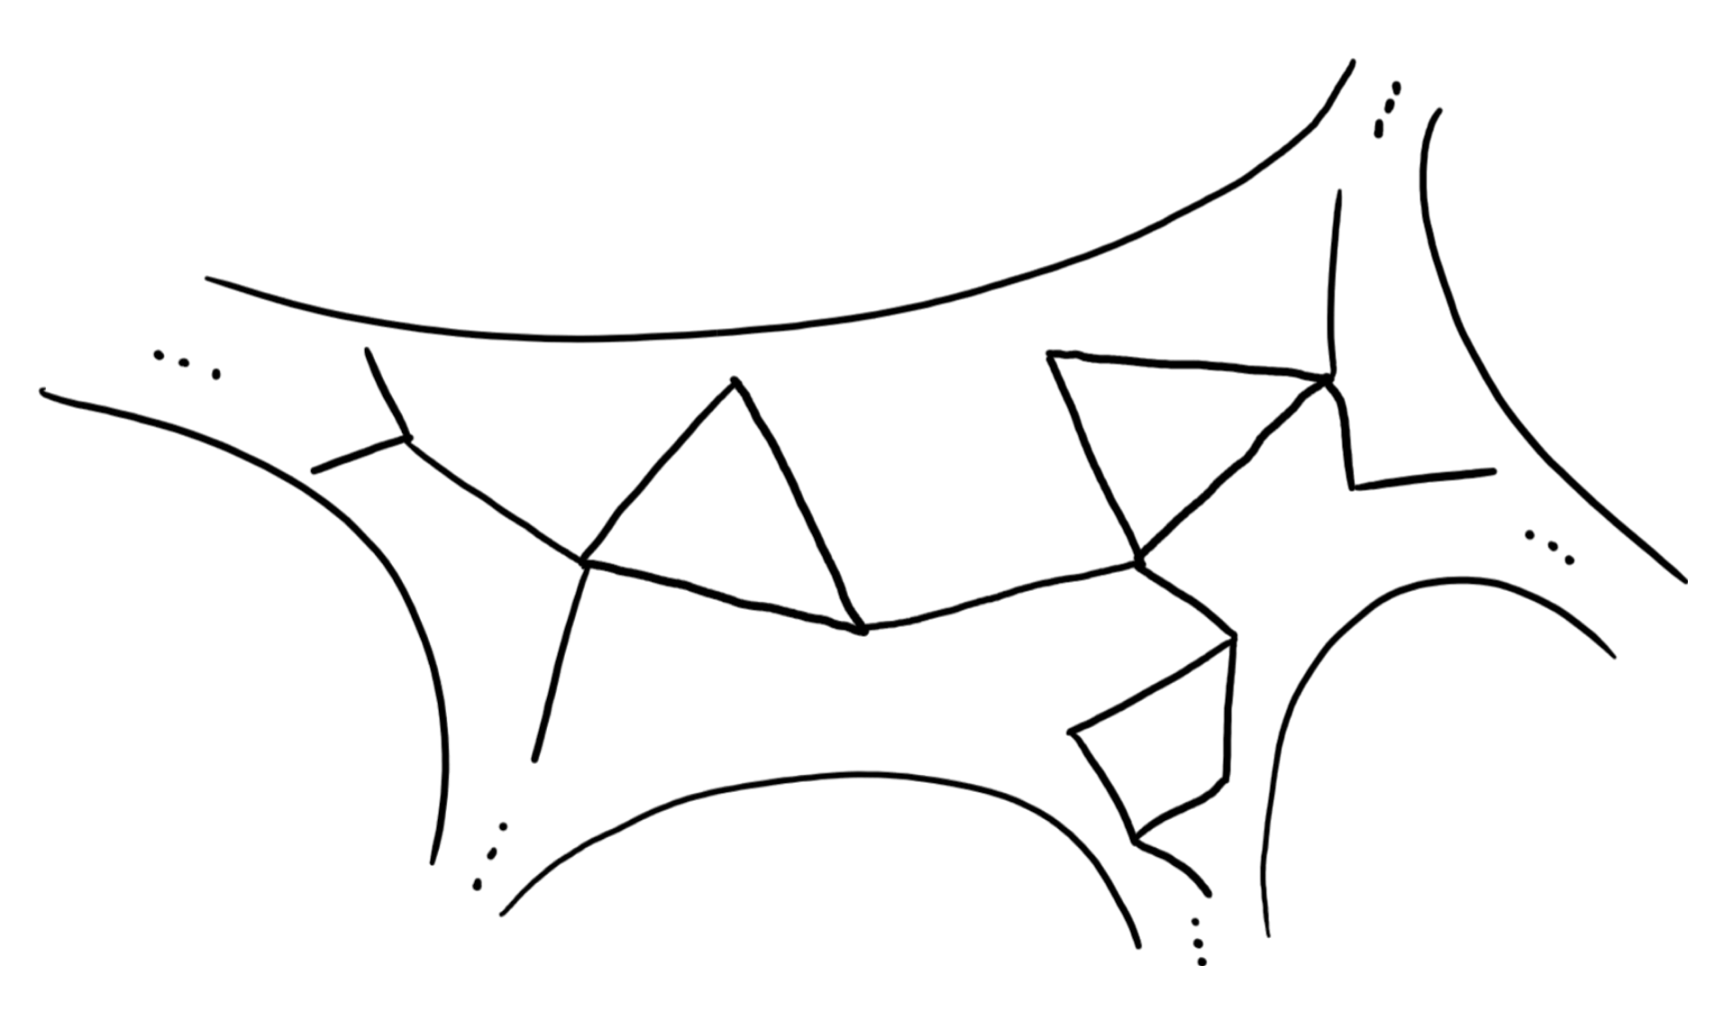
\includegraphics[width=0.9\textwidth]{img/plan/0_base.png}};}}
                    \onslide<5-8>{{\transparent{0.1}\node[inner sep=0pt] at (5,-5) {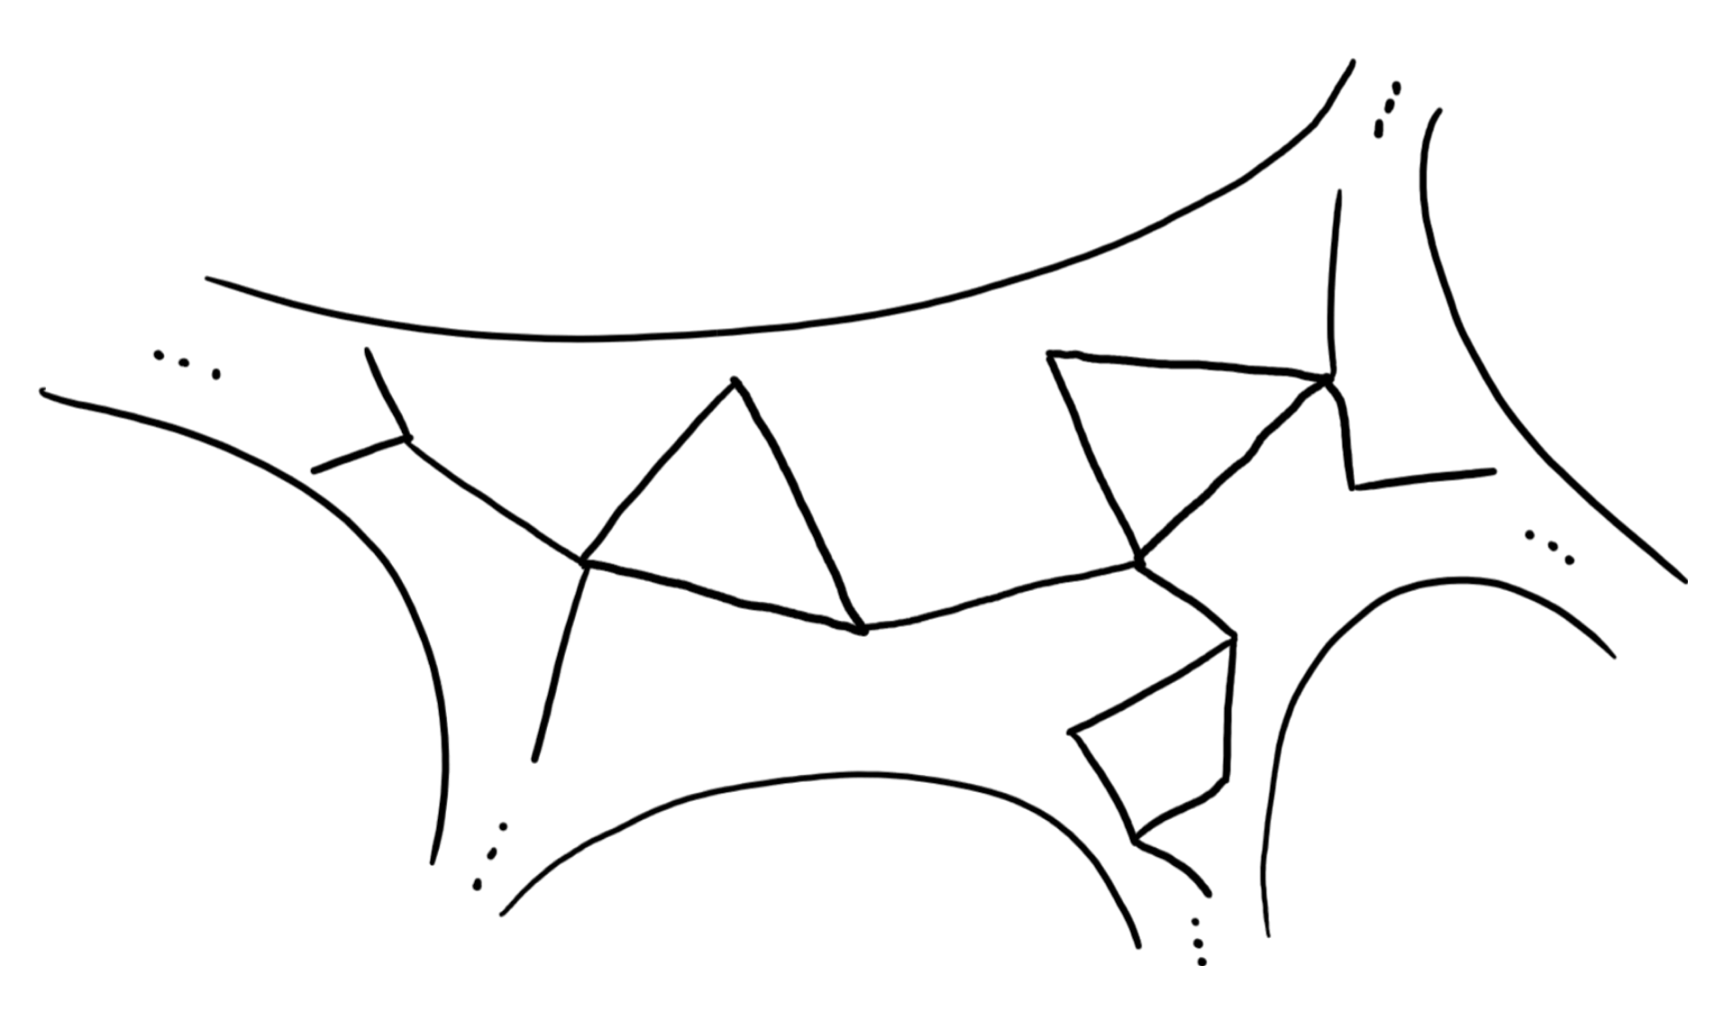
\includegraphics[width=0.9\textwidth]{img/plan/0_base.png}};}}

                    \draw[->] (0,-0.2) -- (0,-\vsp+0.3);
                    \draw (0,\vsh-\vsp) circle (0in) node{Quasi-tree};

                    \pause

                    \draw (\hsp,-\vsp) circle (0in) node{$\begin{gathered} \textrm{Finitely-sep.}\\[-4pt] \textrm{family of cuts} \end{gathered}$};
                    \draw[->] (1,\vsh-\vsp) -- (\hsp-1.1,\vsh-\vsp);

                    \only<3>{\node[inner sep=0pt] at (4.657,-5.34) {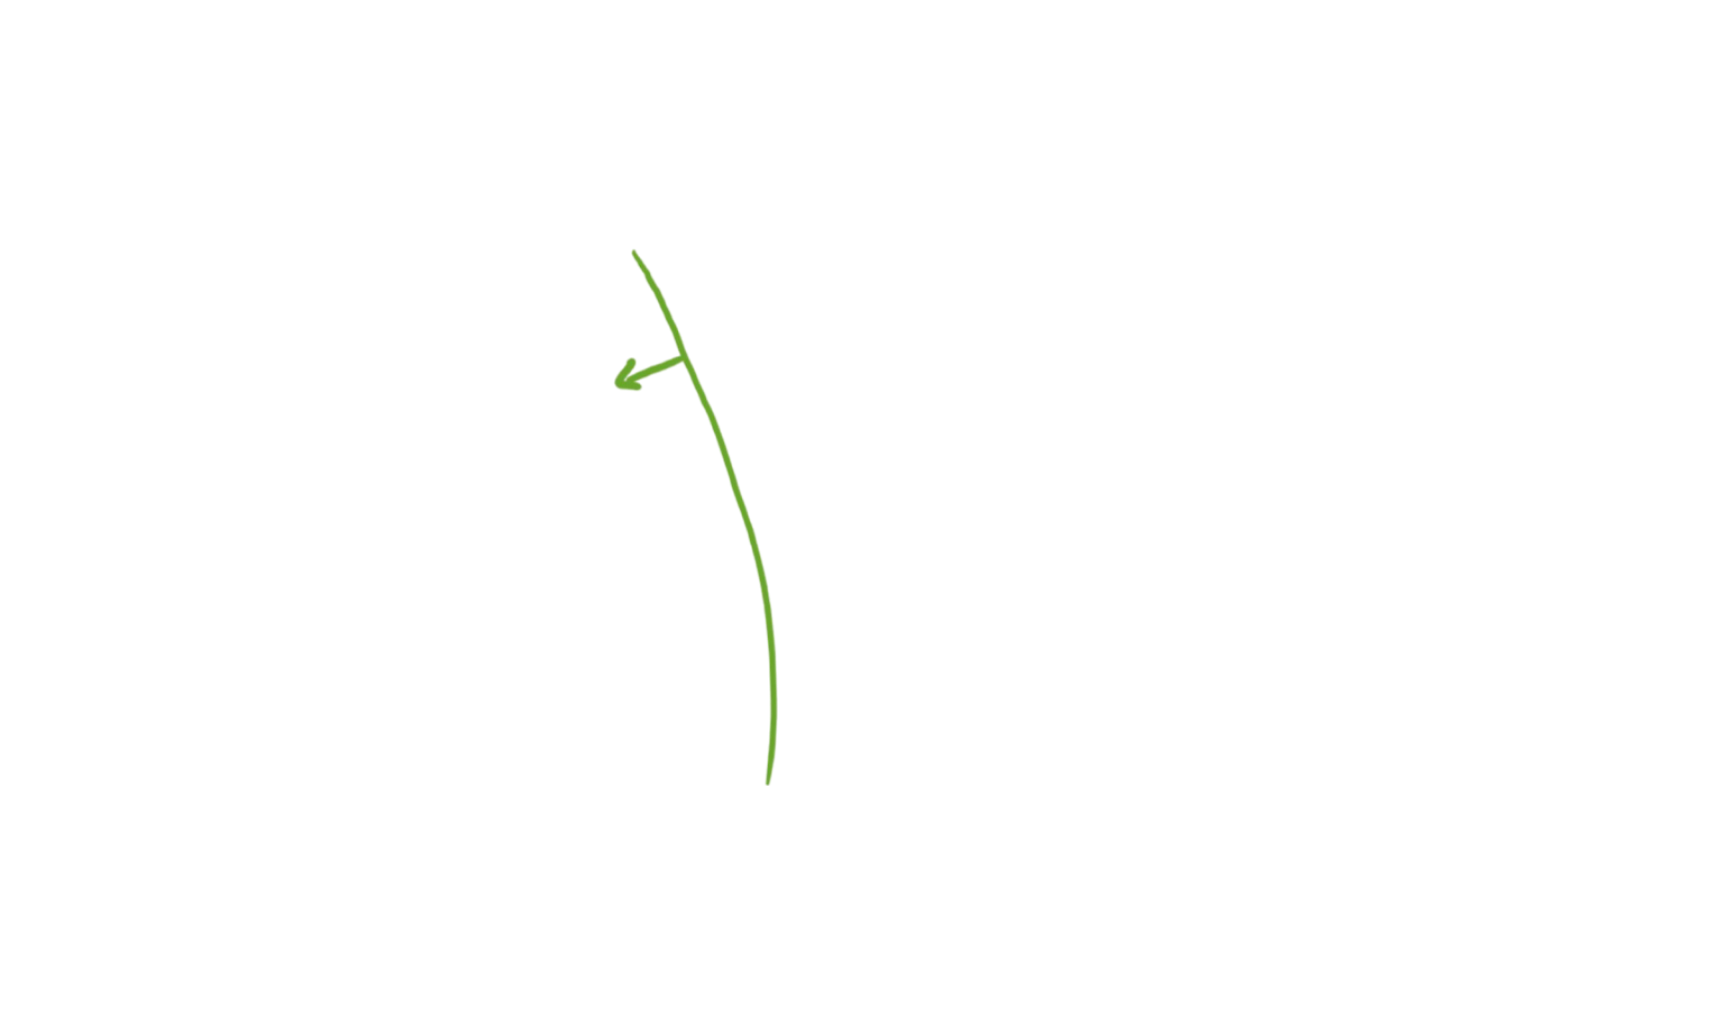
\includegraphics[width=0.9\textwidth]{img/plan/1_cut.png}};}

                    \pause

                    \onslide<4,7>{\node[inner sep=0pt] at (5.8,-5.35) {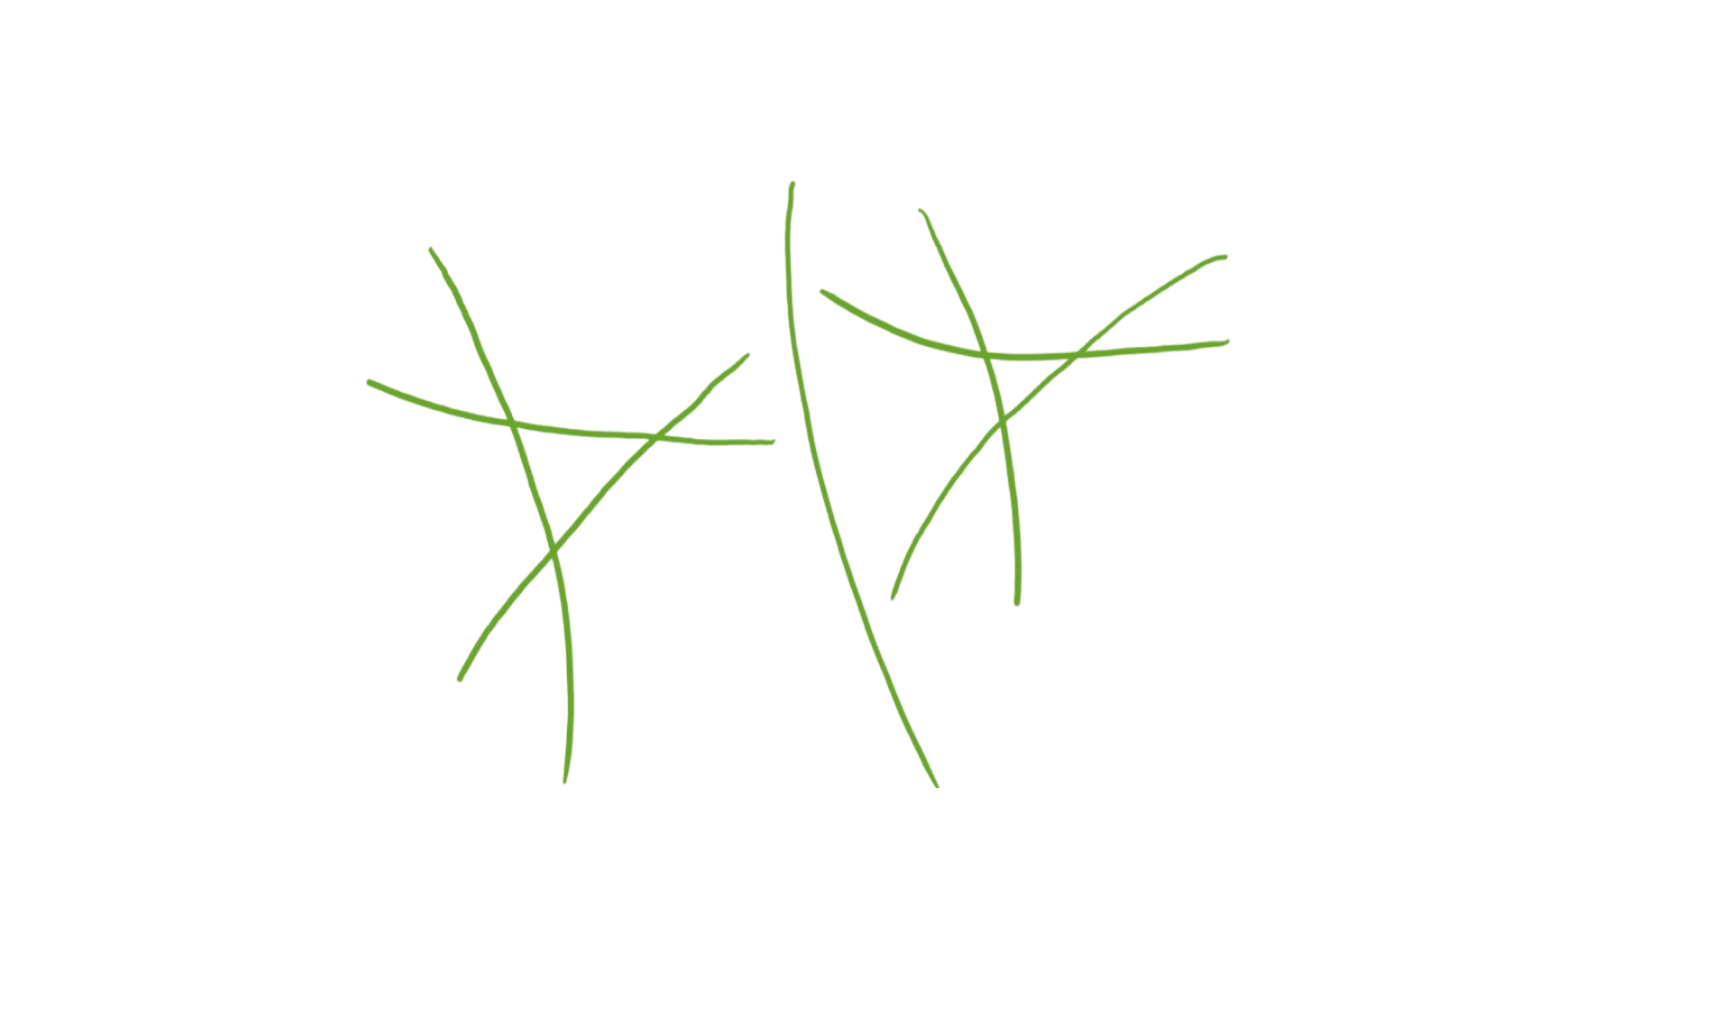
\includegraphics[width=0.9\textwidth]{img/plan/2_cuts.png}};}
                    \only<5>{{\transparent{0.6}\node[inner sep=0pt] at (5.8,-5.35) {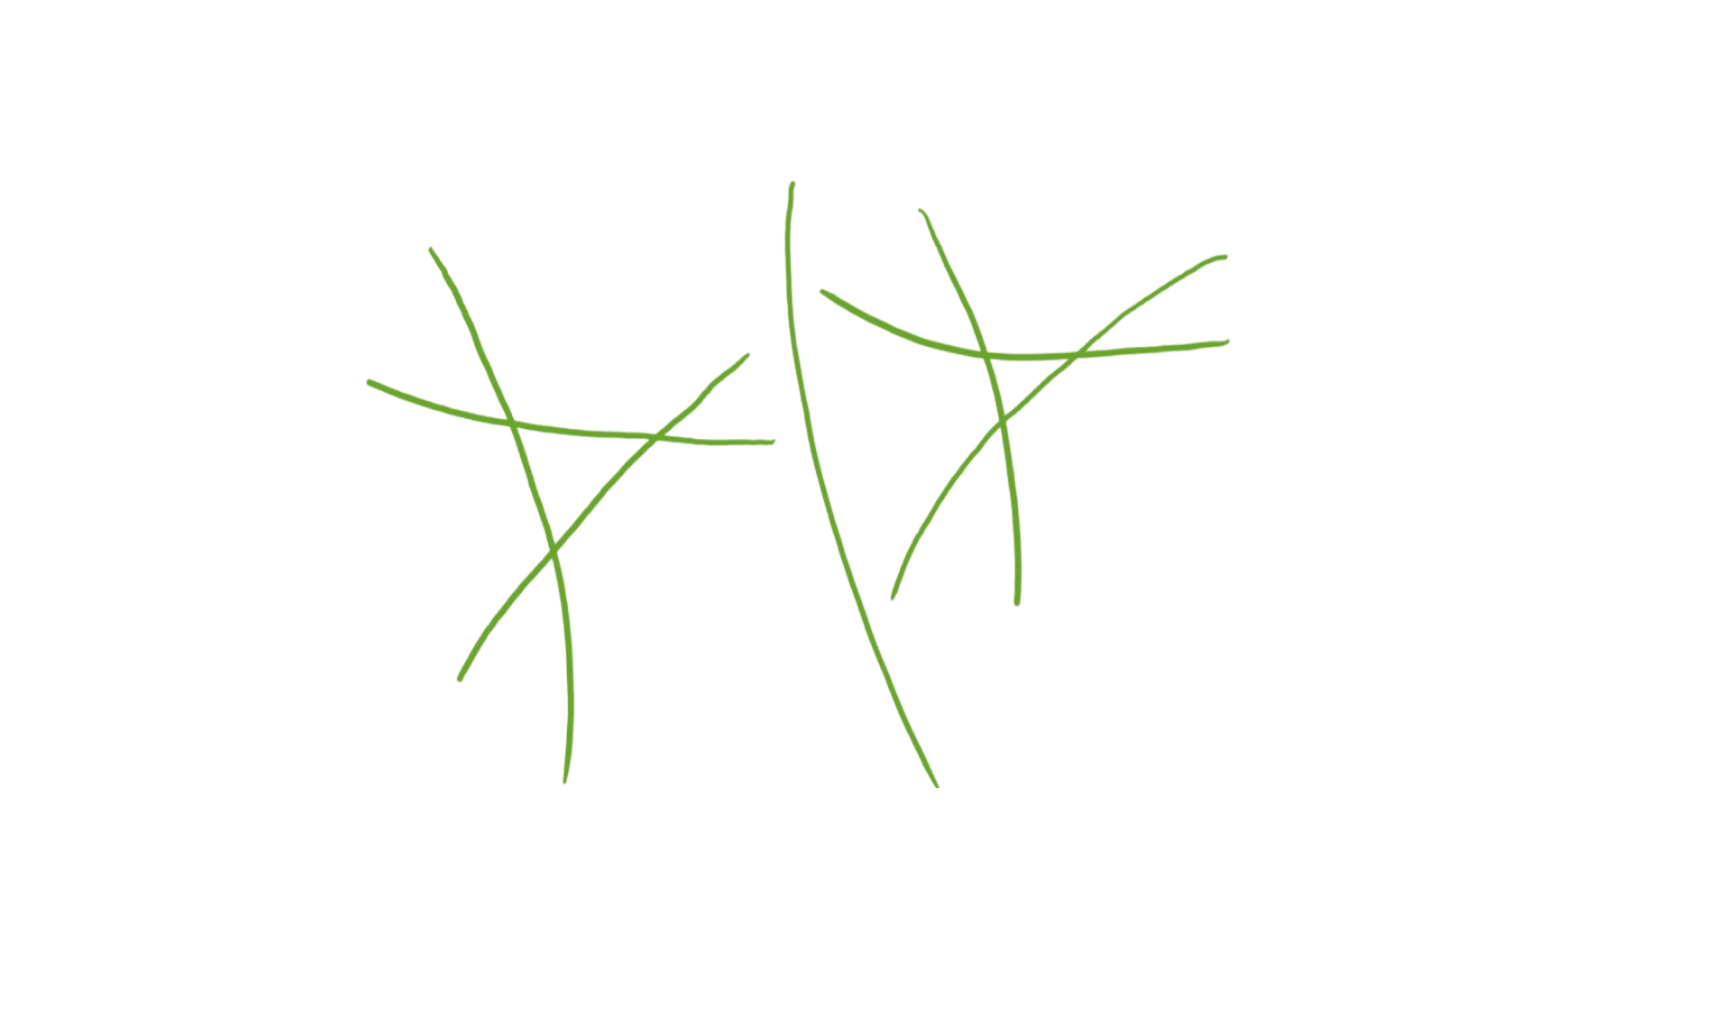
\includegraphics[width=0.9\textwidth]{img/plan/2_cuts.png}};}}
                    \onslide<6,8>{{\transparent{0.3}\node[inner sep=0pt] at (5.8,-5.35) {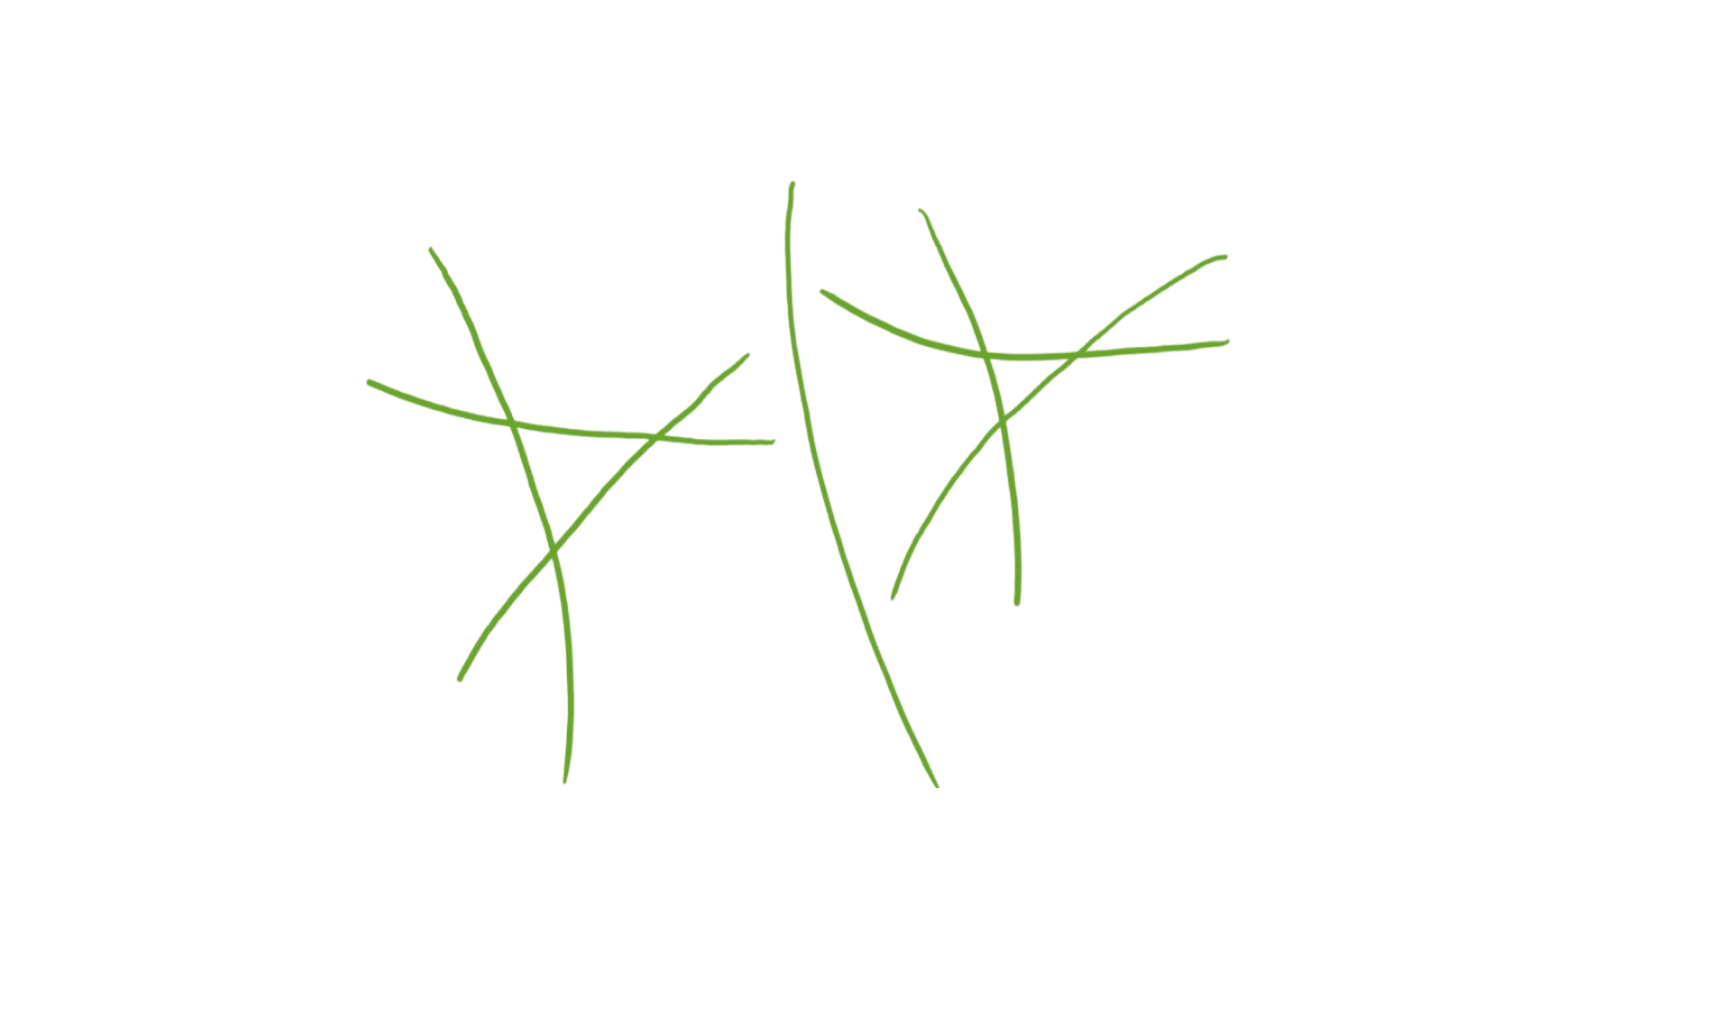
\includegraphics[width=0.9\textwidth]{img/plan/2_cuts.png}};}}

                    \pause

                    \draw (2*\hsp,-\vsp) circle (0in) node{$\begin{gathered} \textrm{Median graph w/}\\[-4pt] \textrm{finite hyperplanes} \end{gathered}$};
                    \draw[->] (\hsp+1.1,\vsh-\vsp) -- (2*\hsp-1.5,\vsh-\vsp);

                    \only<5>{\node[inner sep=0pt] at (5.5,-5) {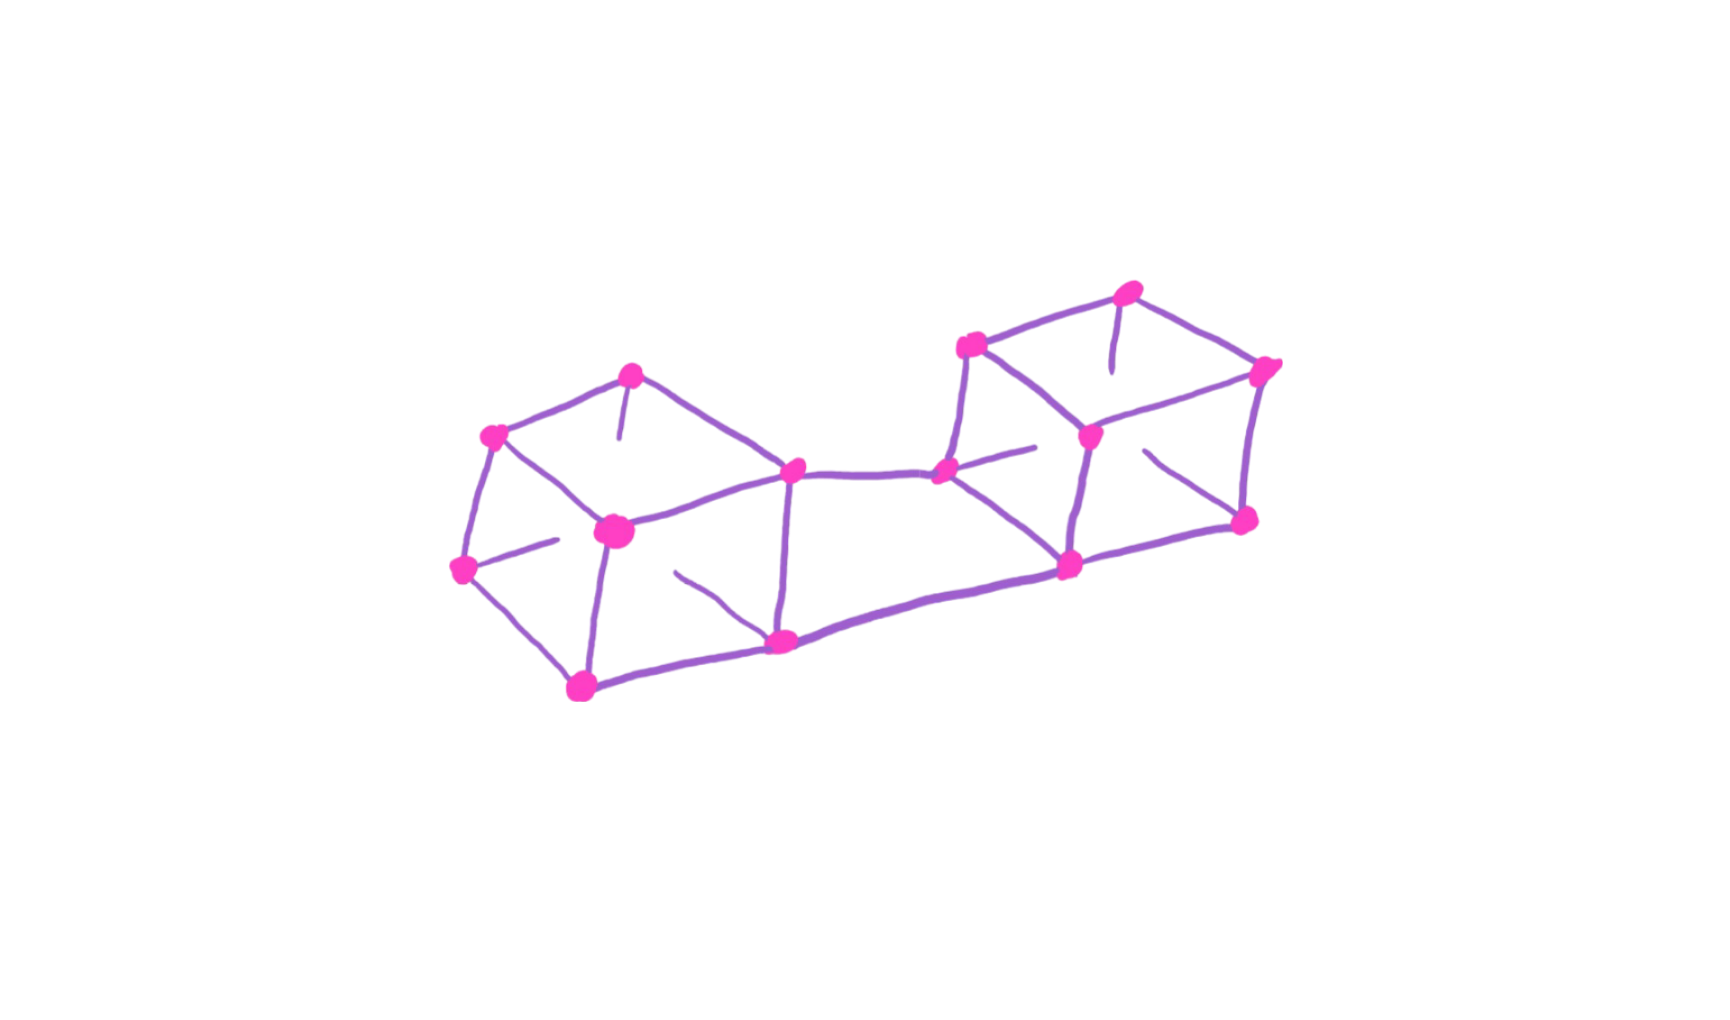
\includegraphics[width=0.83\textwidth]{img/plan/3_median.png}};}
                    \onslide<6-8>{{\transparent{0.4}\node[inner sep=0pt] at (5.5,-5) {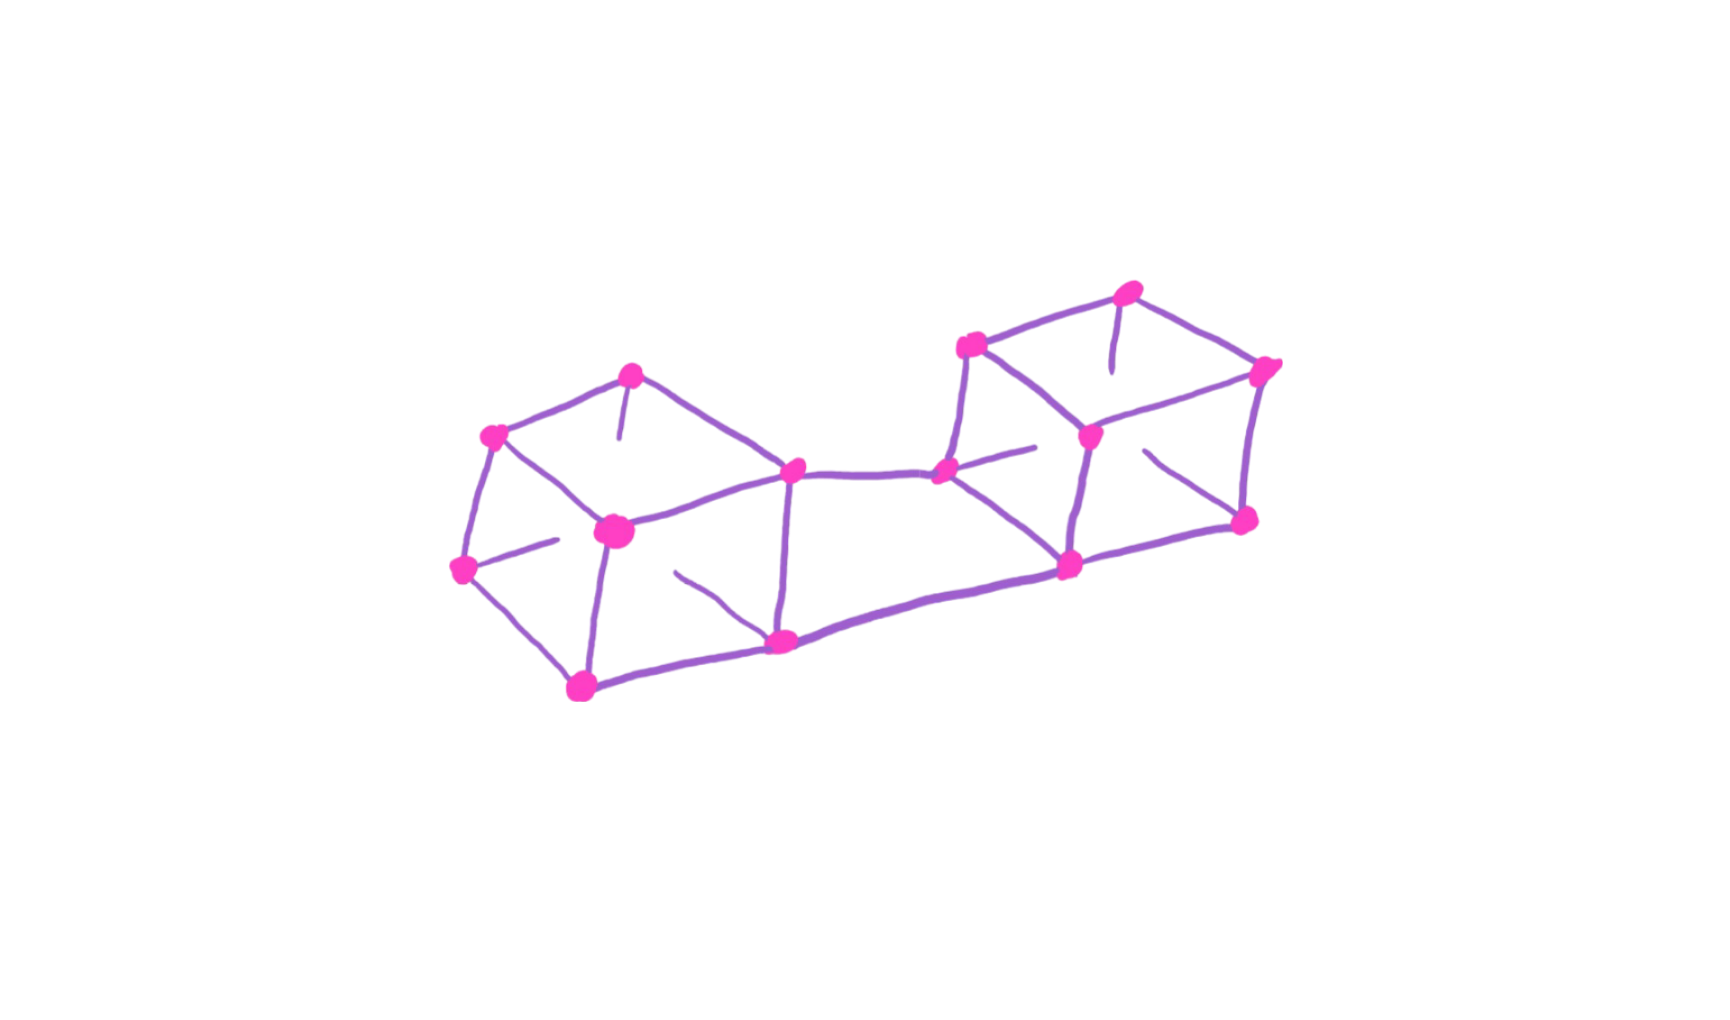
\includegraphics[width=0.83\textwidth]{img/plan/3_median.png}};}}

                    \pause

                    \draw (3*\hsp,-\vsp) circle (0in) node{$\begin{gathered} \textrm{`Canonical'}\\[-4pt] \textrm{spanning tree} \end{gathered}$};
                    \draw[->] (2*\hsp+1.5,\vsh-\vsp) -- (3*\hsp-1.1,\vsh-\vsp);

                    \onslide<6,8>{\node[inner sep=0pt] at (5.76,-4.65) {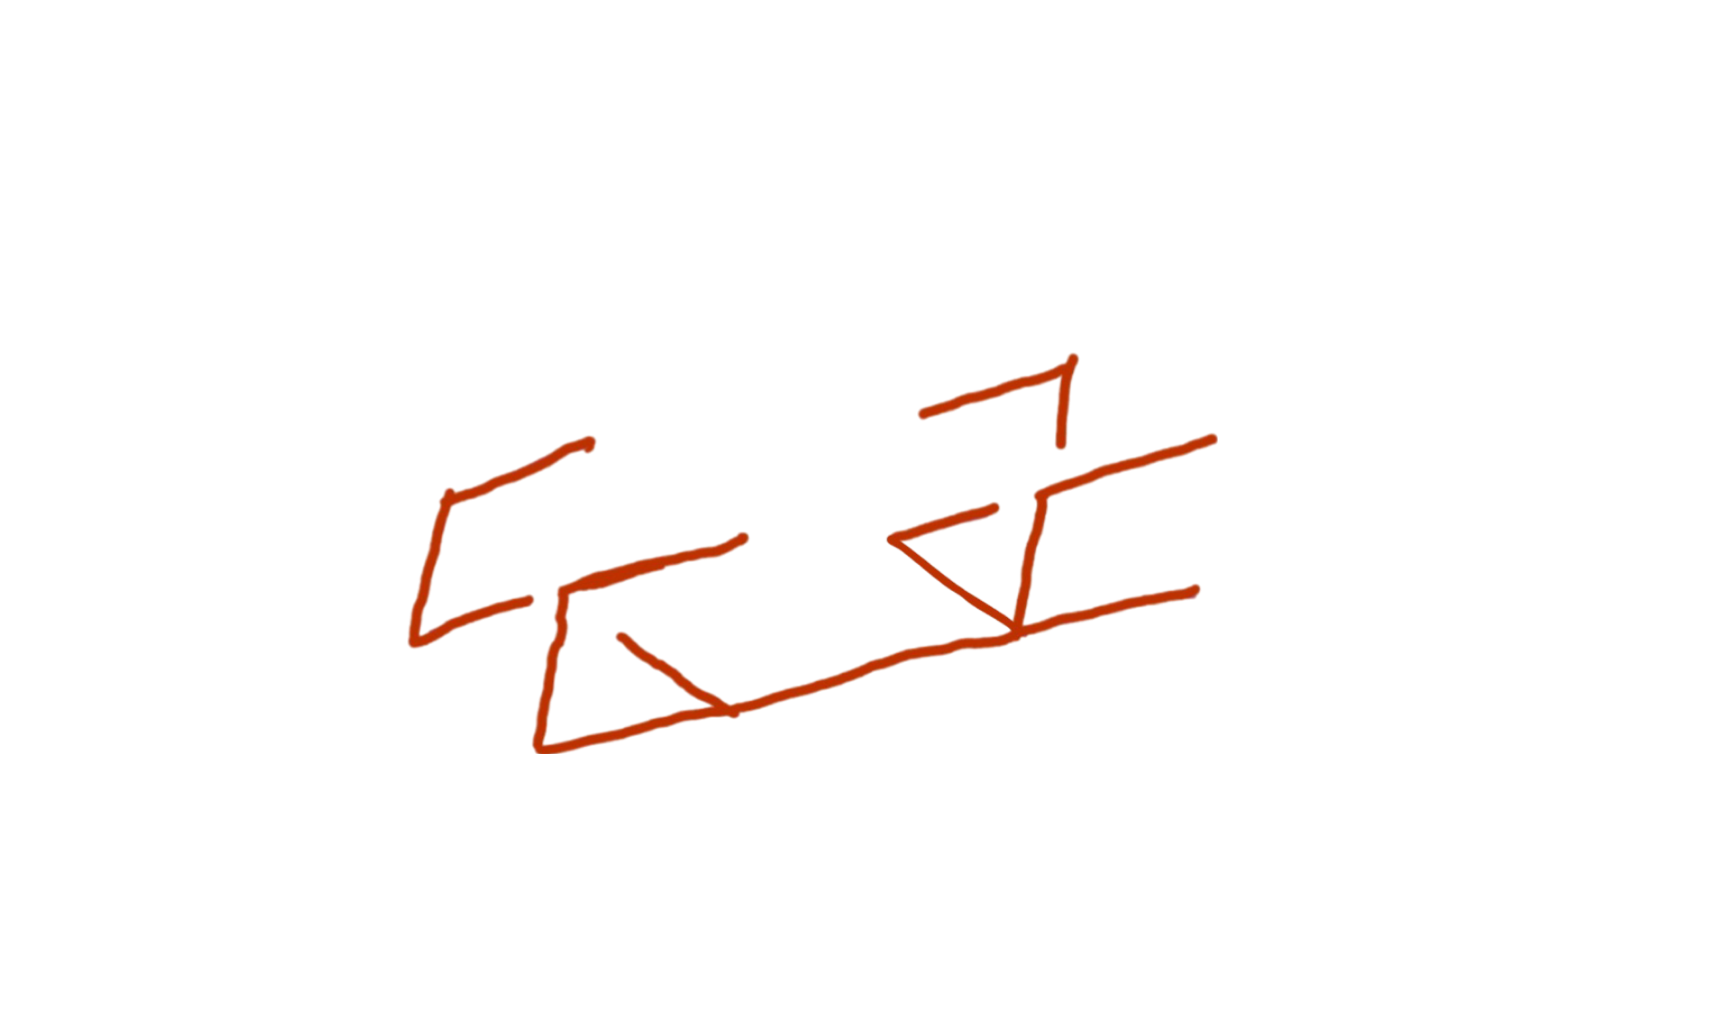
\includegraphics[width=0.83\textwidth]{img/plan/4_tree.png}};}
                    \only<7>{{\transparent{0.2}{\node[inner sep=0pt] at (5.76,-4.65) {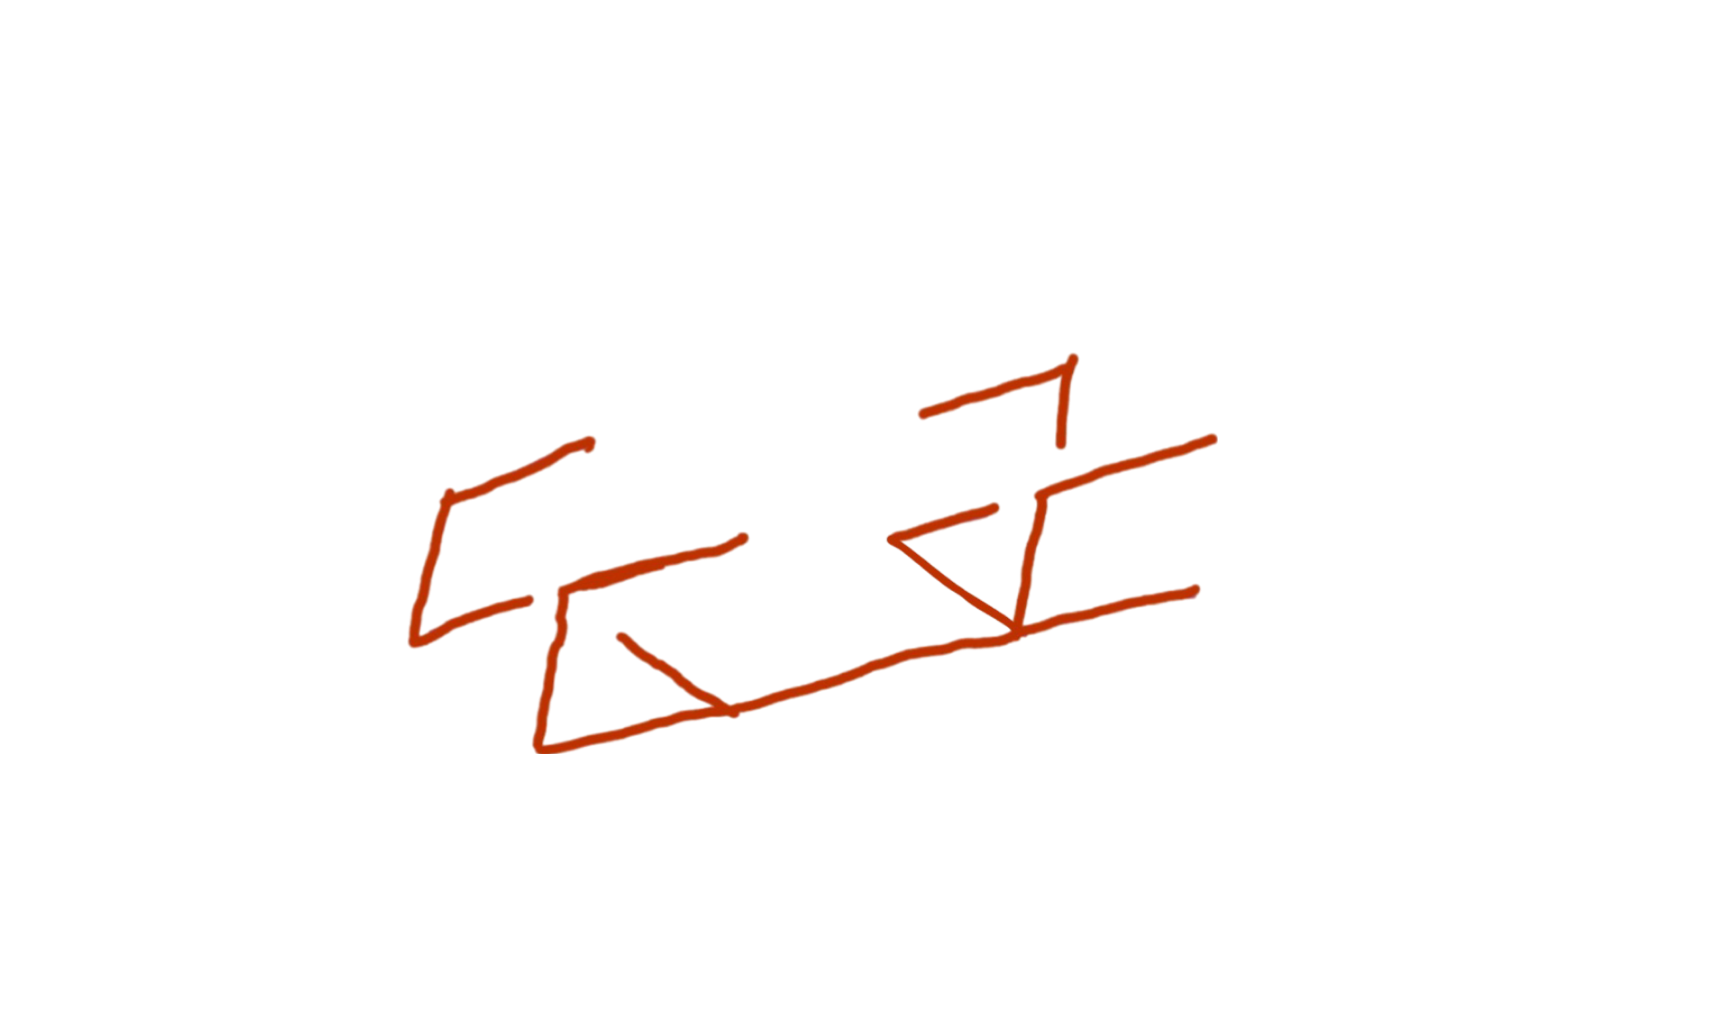
\includegraphics[width=0.83\textwidth]{img/plan/4_tree.png}};}}}

                    \pause

                    \draw (\hsp,0) circle (0in) node{$\begin{gathered} \textrm{Dense family}\\[-4pt] \textrm{of cuts} \end{gathered}$};
                    \draw[->] (1,-1) -- (\hsp-1.1,0);

                    \node[inner sep=0pt] at (5.1,-5.2) {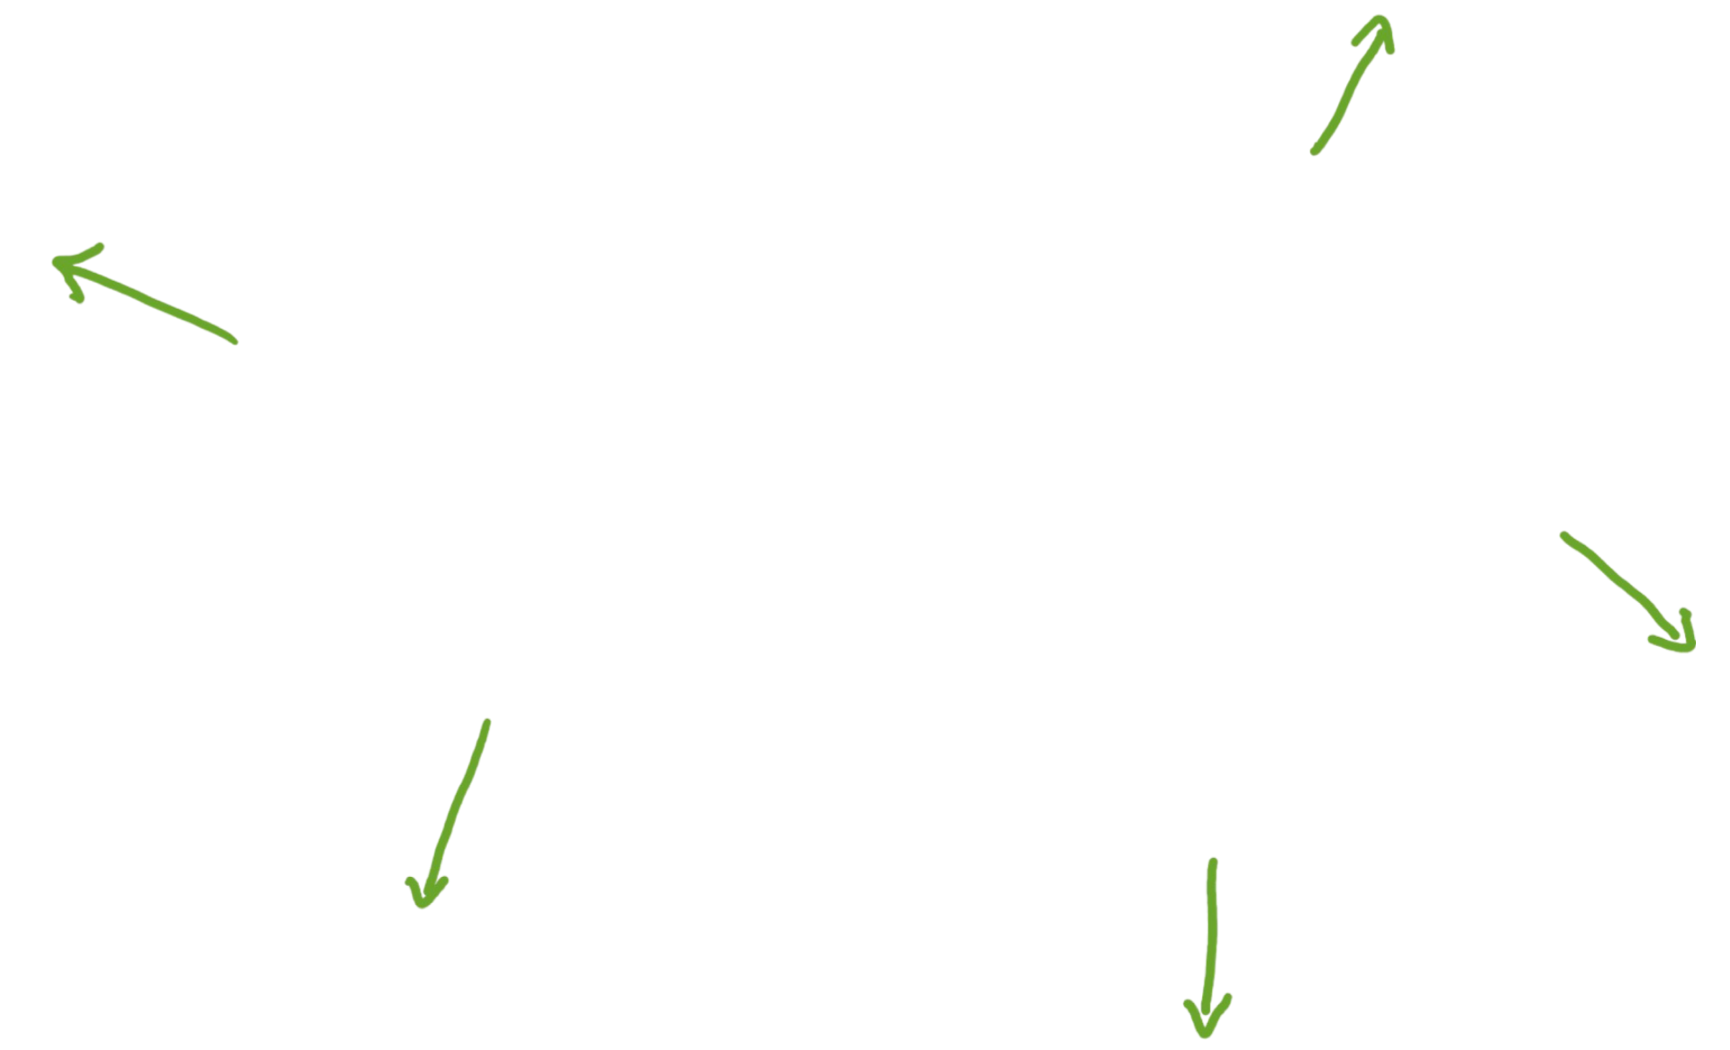
\includegraphics[width=0.9\textwidth]{img/plan/5_ends.png}};

                    \pause

                    \draw[->] (\hsp+1.1,\vsh) -- (3*\hsp-1.1,\vsh);
                    \draw[->] (3*\hsp,0.4-\vsp) -- (3*\hsp,-0.2);
                    \draw (\hsp+1.1,-1) to [out=35, in=180] (2*\hsp,\vsh);
                \end{tikzpicture}
            }
        \end{center}
    \end{frame}
    \begin{frame}{Finitely-separating cuts}
        \begin{definition}
            A \textit{cut} in a connected locally-finite graph $(X,G)$ is a connected co-connected subset $H\subseteq X$ with finite boundary.
        \end{definition}

        \vspace{-0.2in}

        \begin{center}
        \scalebox{0.5}{
            \begin{tikzpicture}
                {{\transparent{0.5}\node[inner sep=0pt] at (5,-5) {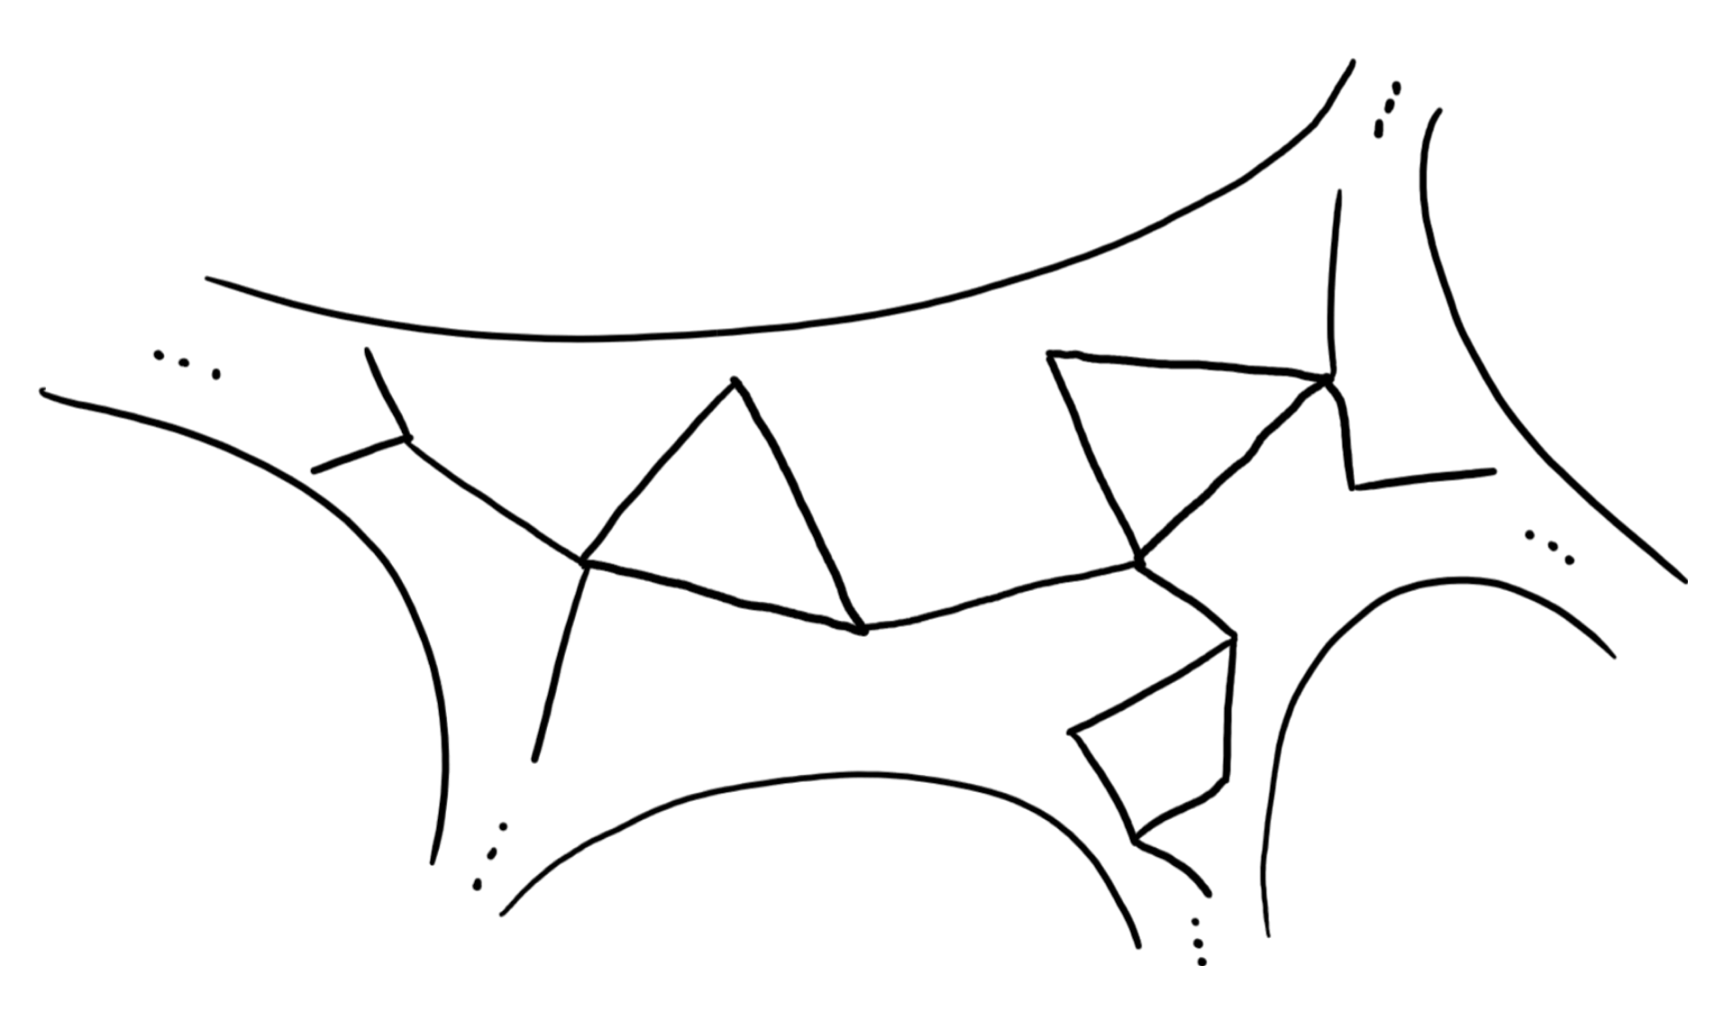
\includegraphics[width=0.9\textwidth]{img/plan/0_base.png}};}}
                \node[inner sep=0pt] at (5.8,-5.35) {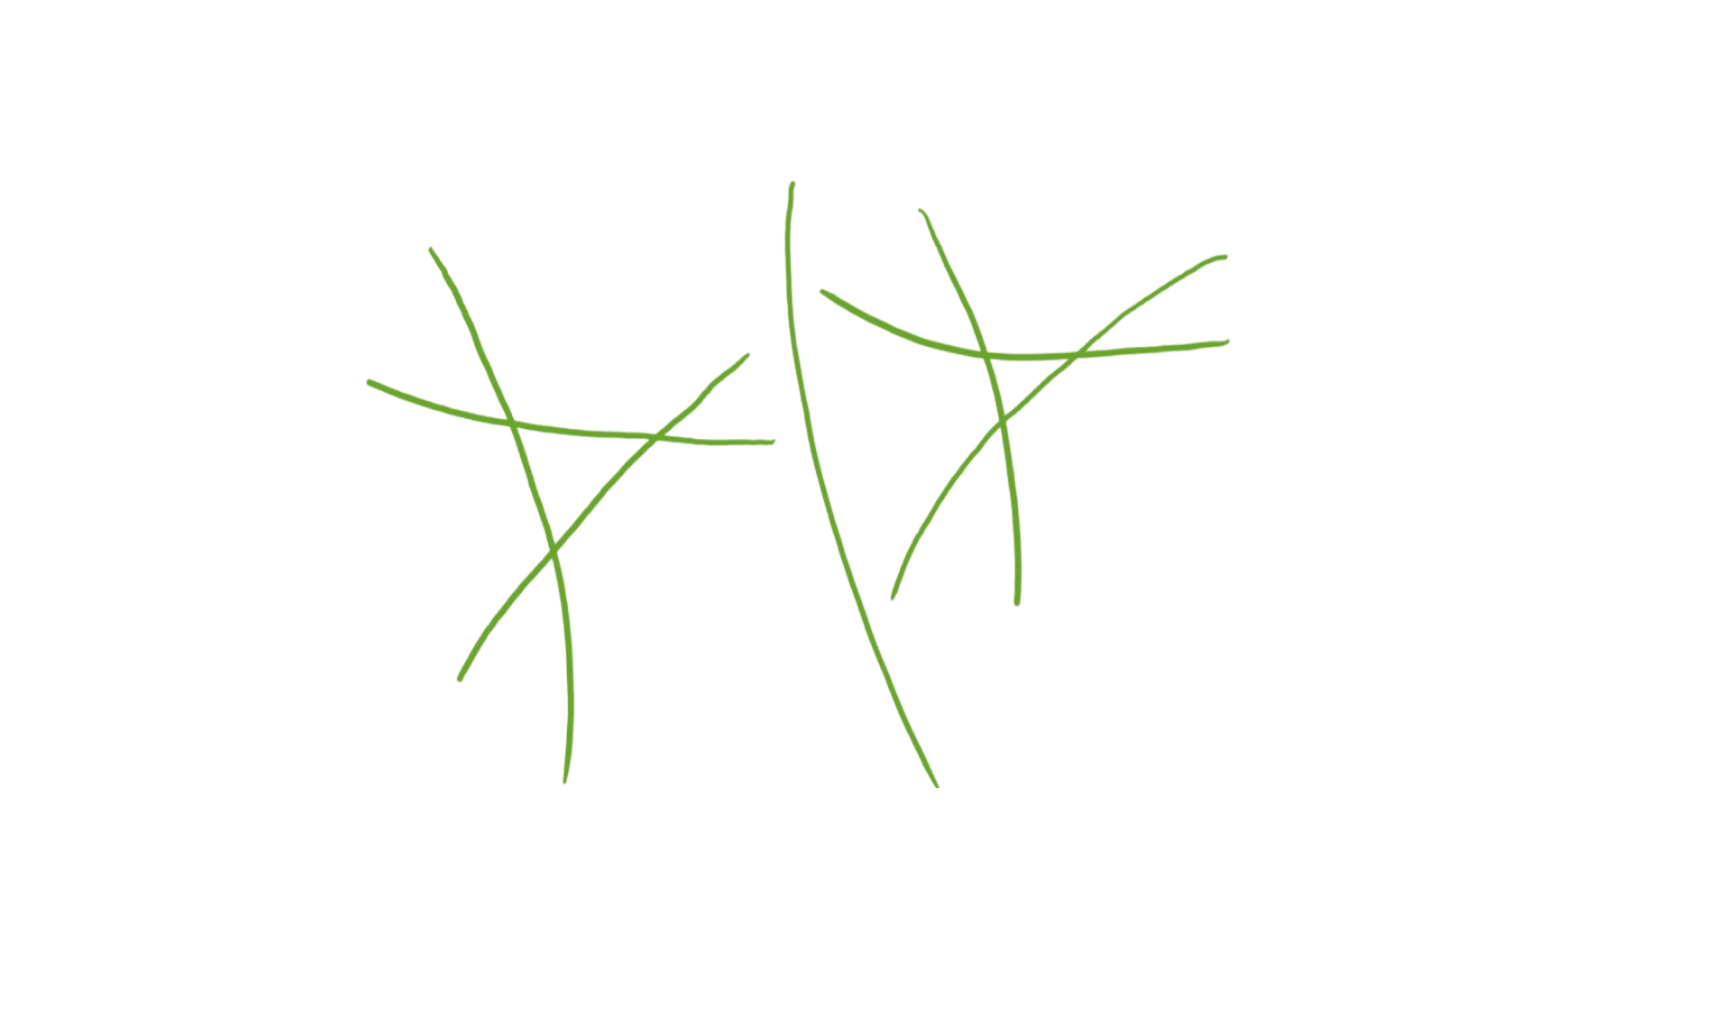
\includegraphics[width=0.9\textwidth]{img/plan/2_cuts.png}};
            \end{tikzpicture}
        }\end{center}

        \vspace{-0.2in}
        \pause

        Let $\mc{H}$ be a family of cuts such that if $H\in\mc{H}$, then $\lnot H\in\mc{H}$.

        \pause

        \begin{definition}
            Such a family $\mc{H}$ is \textit{finitely-separating} if for each $x,y\in X$, there are finitely-many $H\in\mc{H}$ with $x\in H\not\ni y$.
        \end{definition}
    \end{frame}
    \begin{frame}{Orientations}
        \begin{definition}
            An \textit{orientation} on $\mc{H}$ is an upward-closed subset $U\subseteq\mc{H}$ containing exactly one of $H,\lnot H$ for every $H\in\mc{H}$.
        \end{definition}

        \vspace{-0.2in}

        \begin{center}
        \scalebox{0.5}{
            \begin{tikzpicture}
                {{\transparent{0.2}\node[inner sep=0pt] at (5,-5) {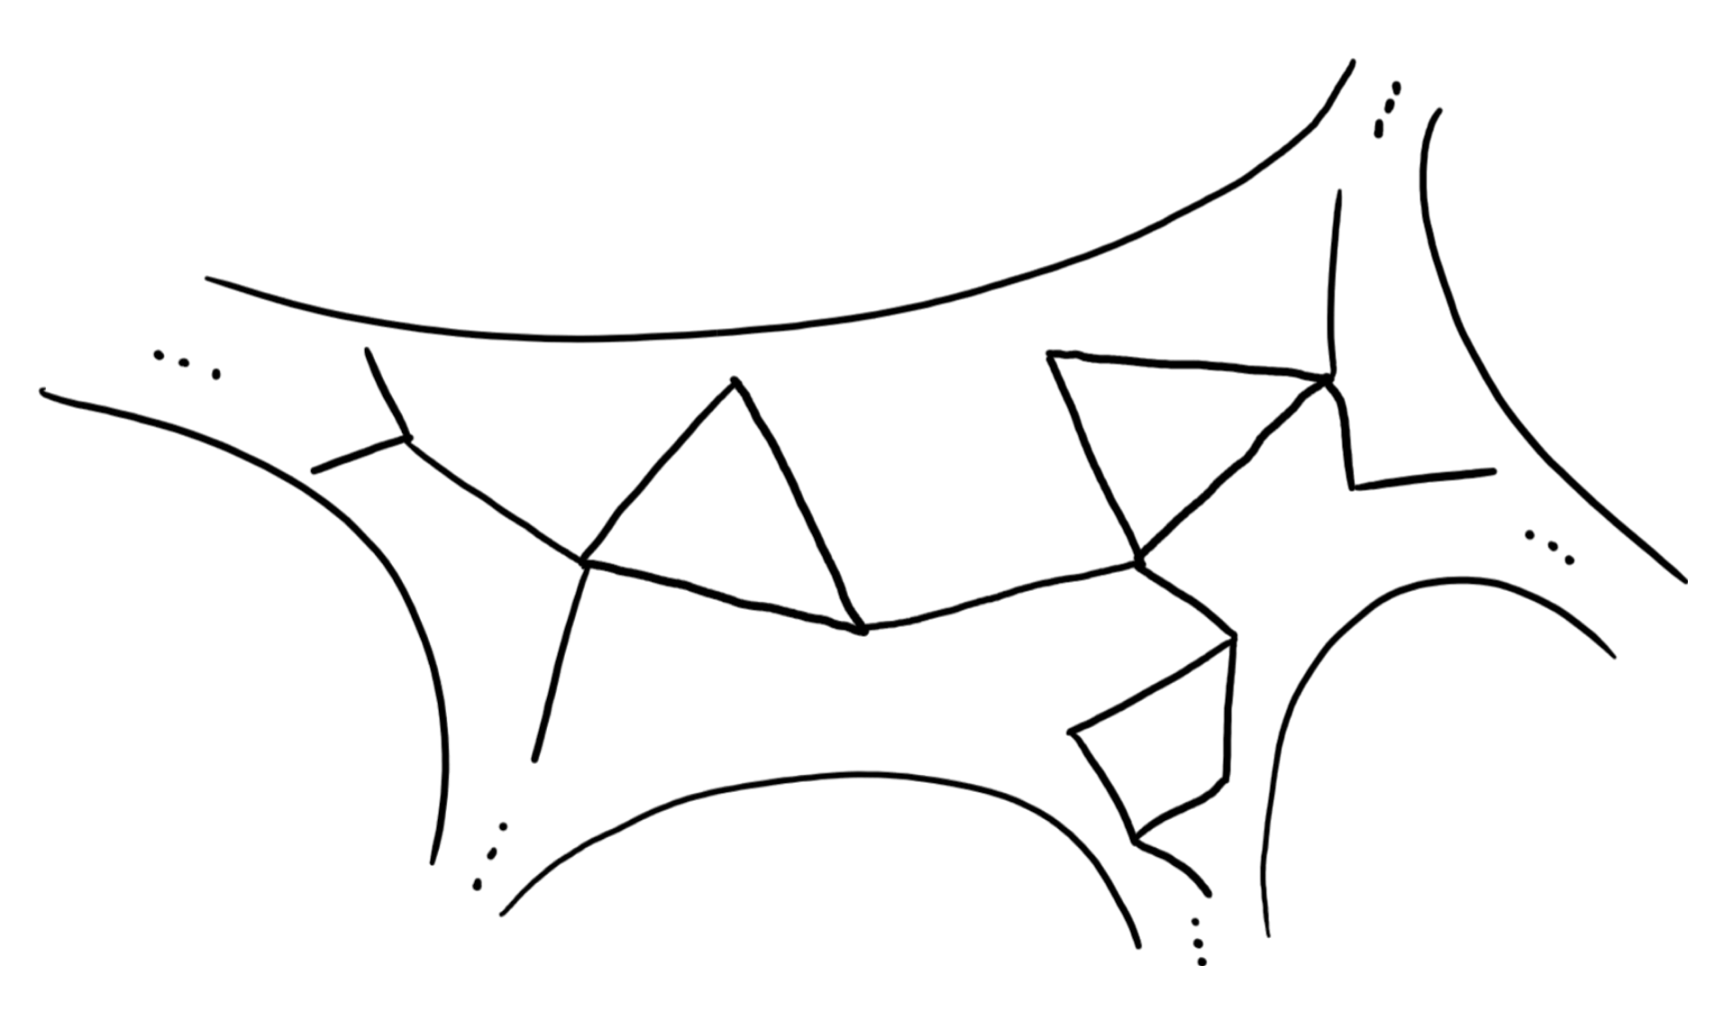
\includegraphics[width=0.9\textwidth]{img/plan/0_base.png}};}}
                {{\transparent{0.5}\node[inner sep=0pt] at (5.8,-5.35) {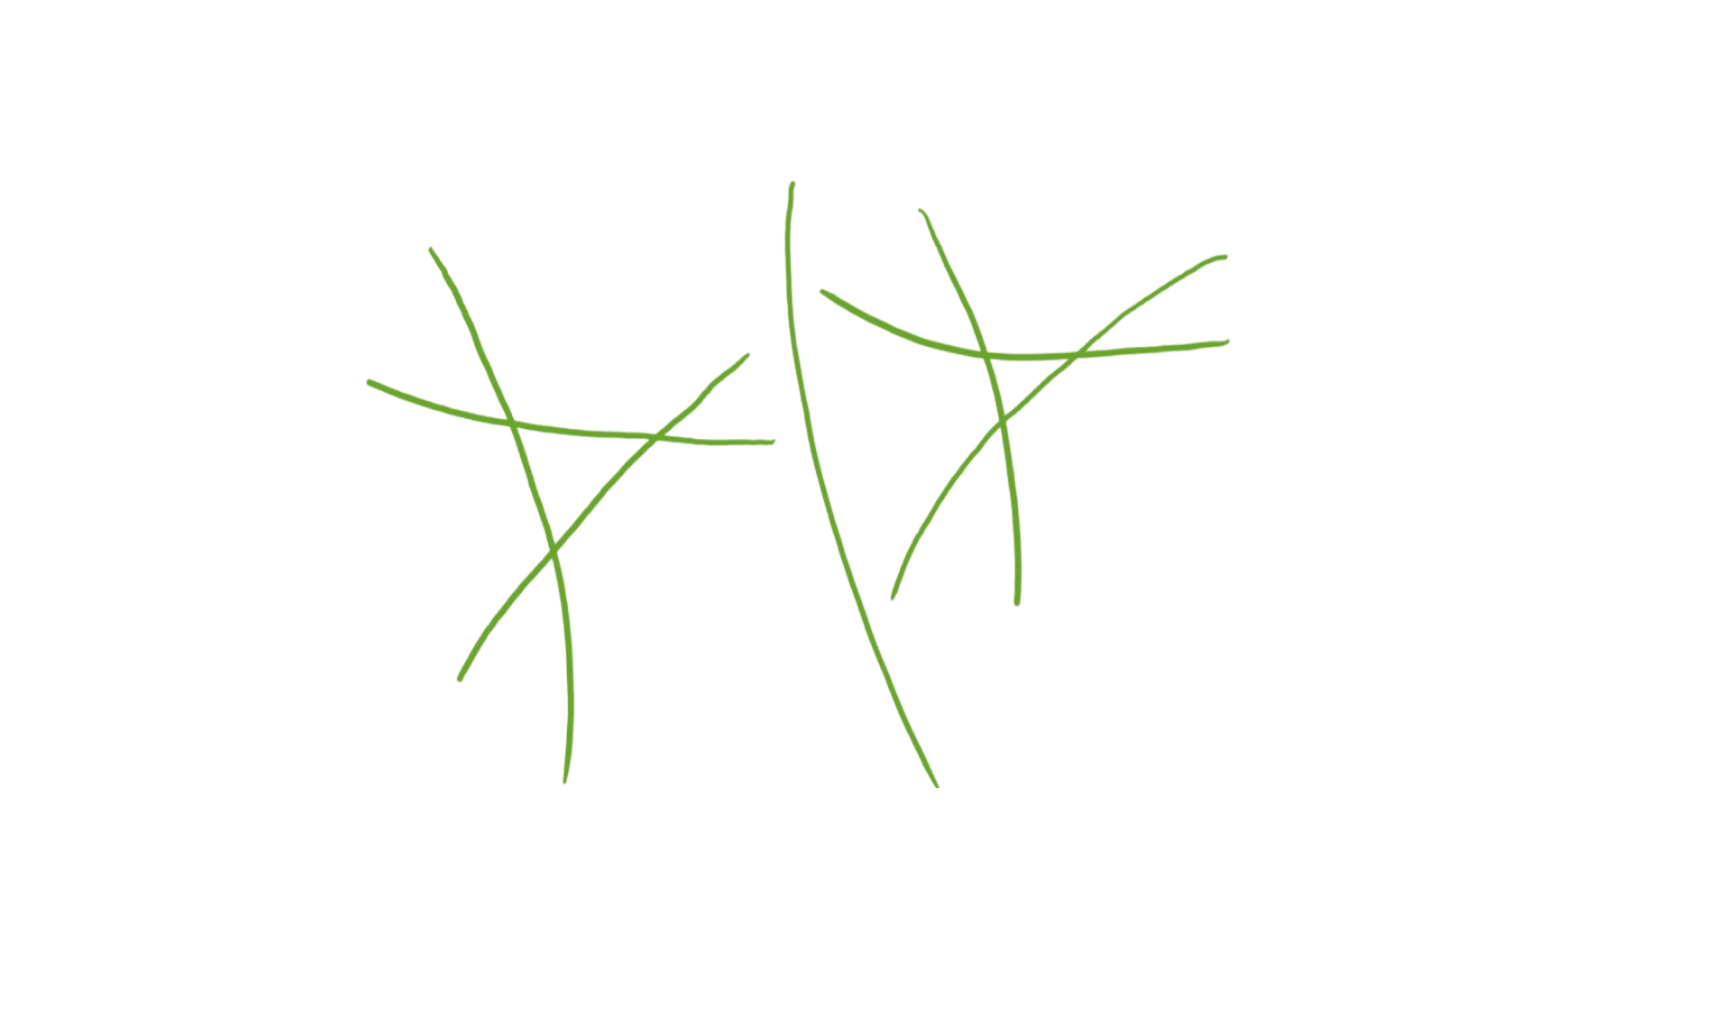
\includegraphics[width=0.9\textwidth]{img/plan/2_cuts.png}};}}
                \node[inner sep=0pt] at (5.5,-5) {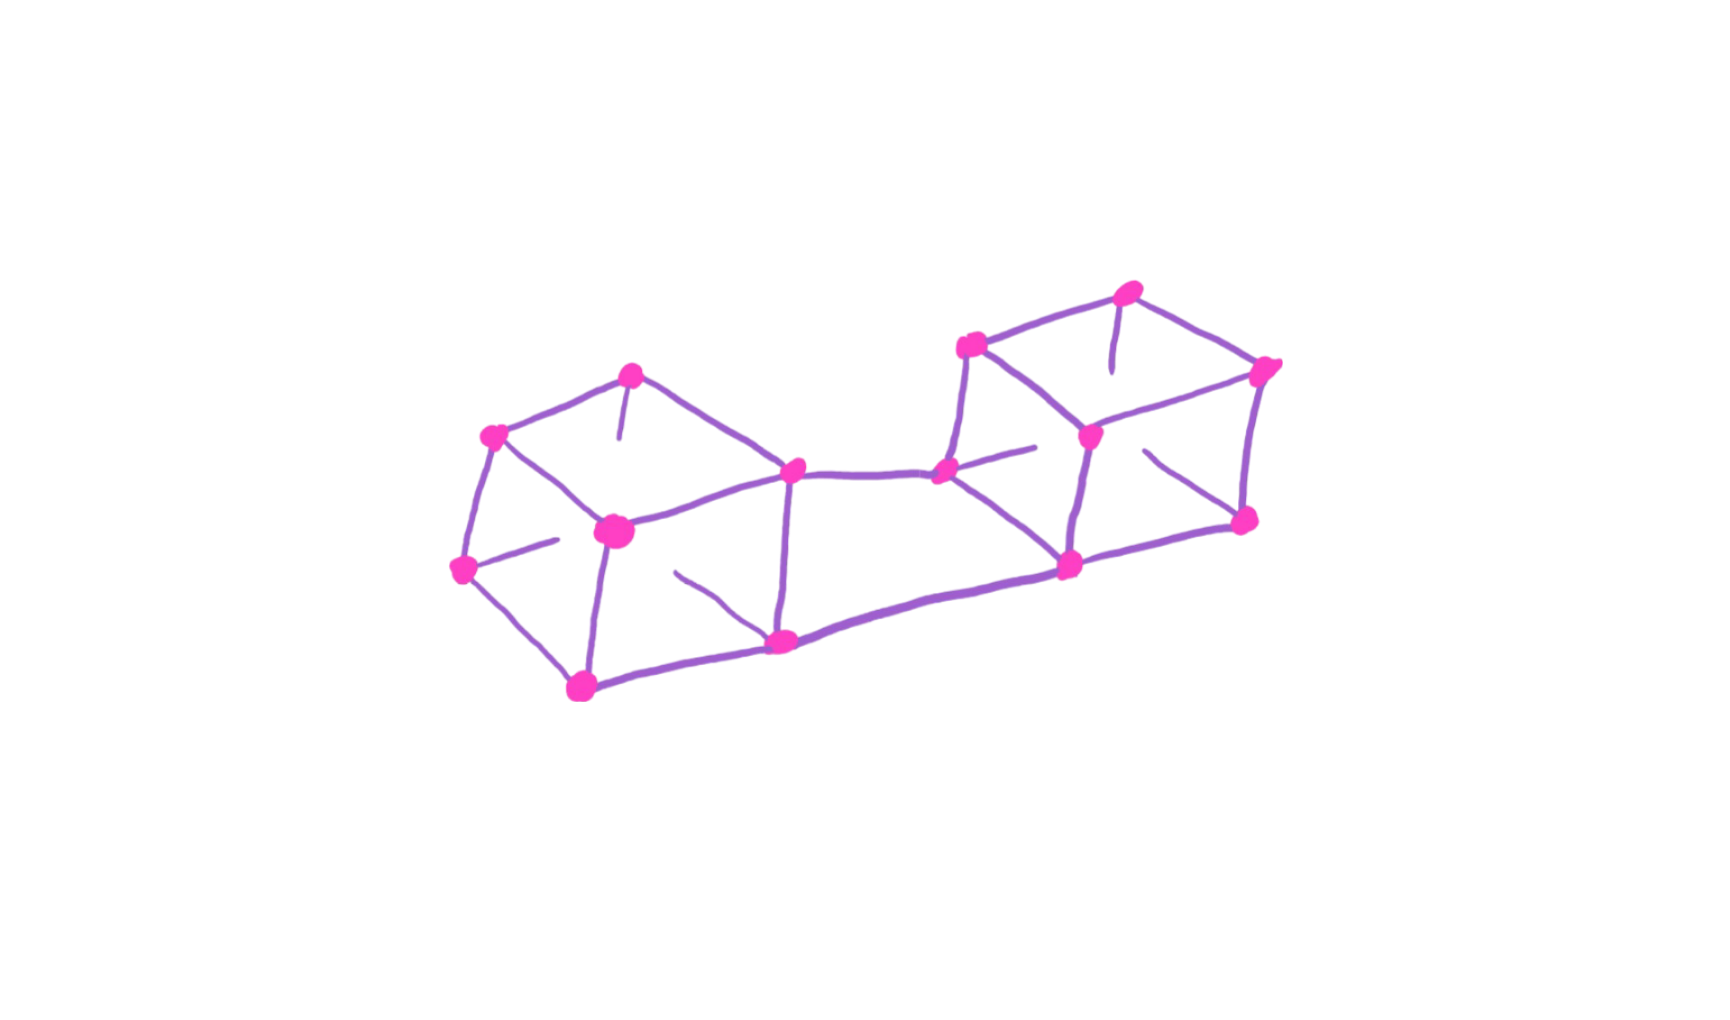
\includegraphics[width=0.83\textwidth]{img/plan/3_median.png}};
            \end{tikzpicture}
        }\end{center}

        \vspace{-0.2in}
        \pause

        We'll only consider the orientations that are \textit{based}, in the sense that each $H\in U$ contains a minimal $H_0\in U$.
    \end{frame}
    \begin{frame}{The dual median graph}
        \begin{definition}
            A \textit{median graph} is a connected graph $(X,G)$ such that for each $x,y,z\in X$, the intersection $[x,y]\cap[x,z]\cap[y,z]$ is a singleton, called the \textit{median} of $x,y,z$, and is denoted by $\l\langle x,y,z\r\rangle$.
        \end{definition}

        \vspace{-0.2in}

        \begin{center}
        \scalebox{0.5}{
            \begin{tikzpicture}
                {{\transparent{0.2}\node[inner sep=0pt] at (5,-5) {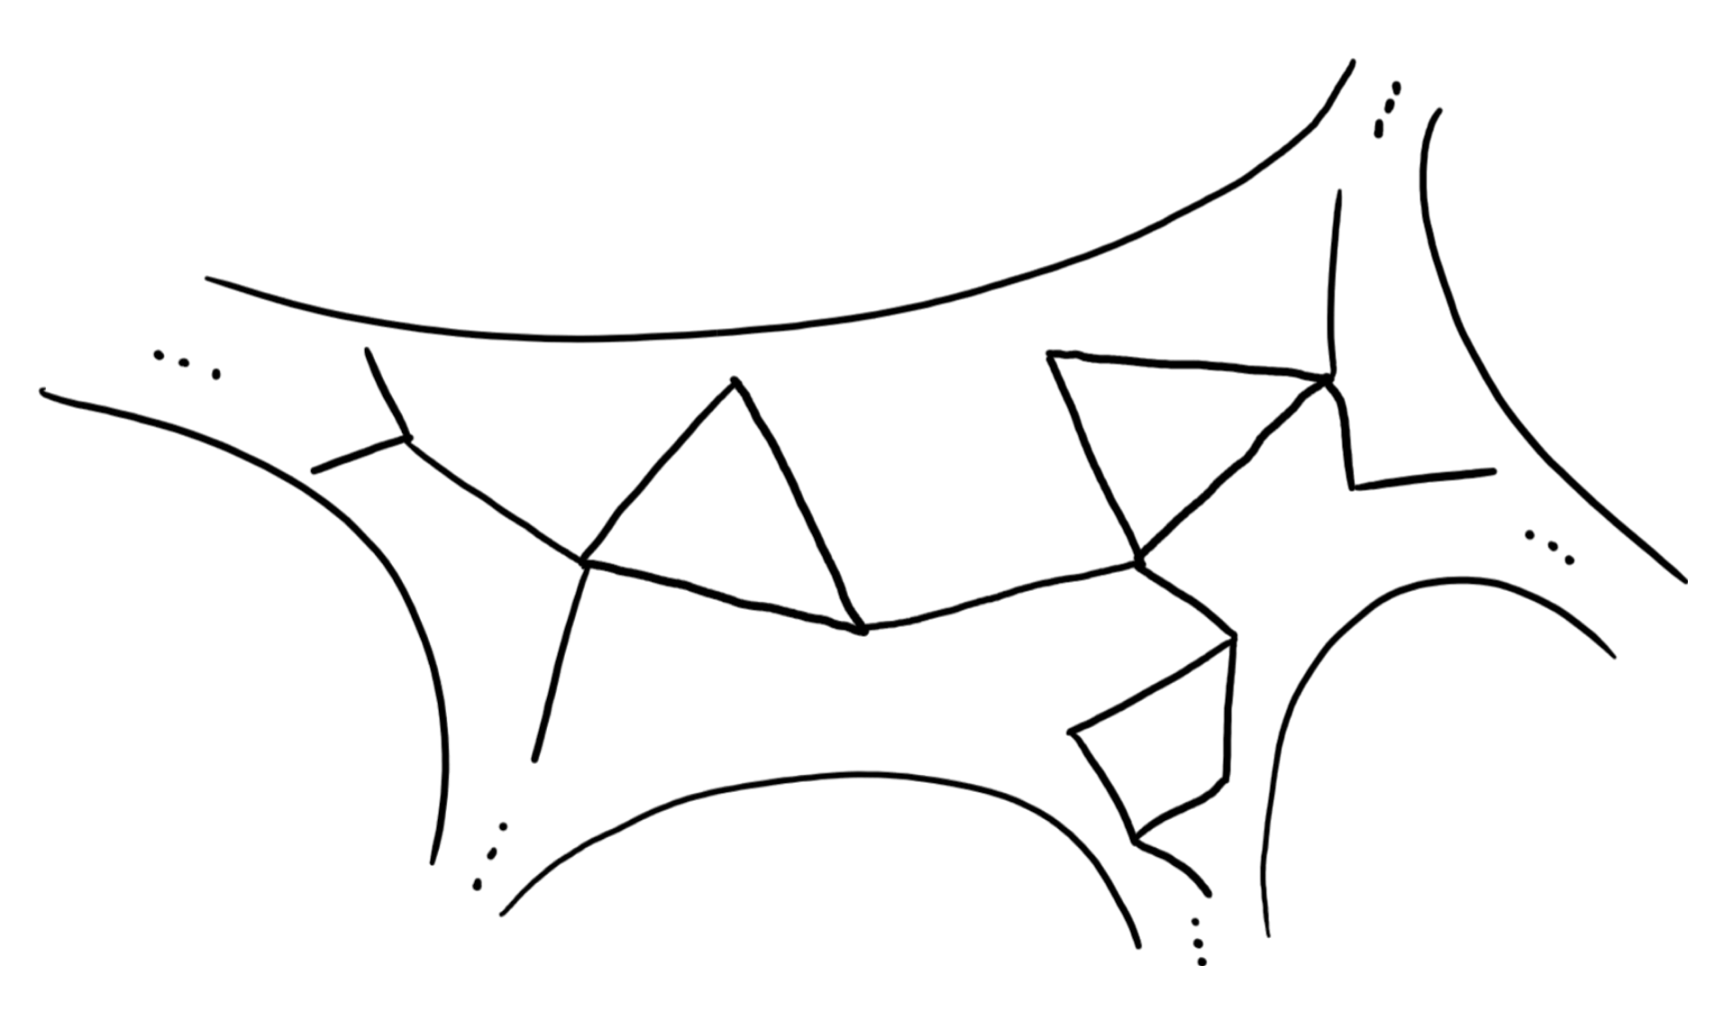
\includegraphics[width=0.9\textwidth]{img/plan/0_base.png}};}}
                {{\transparent{0.5}\node[inner sep=0pt] at (5.8,-5.35) {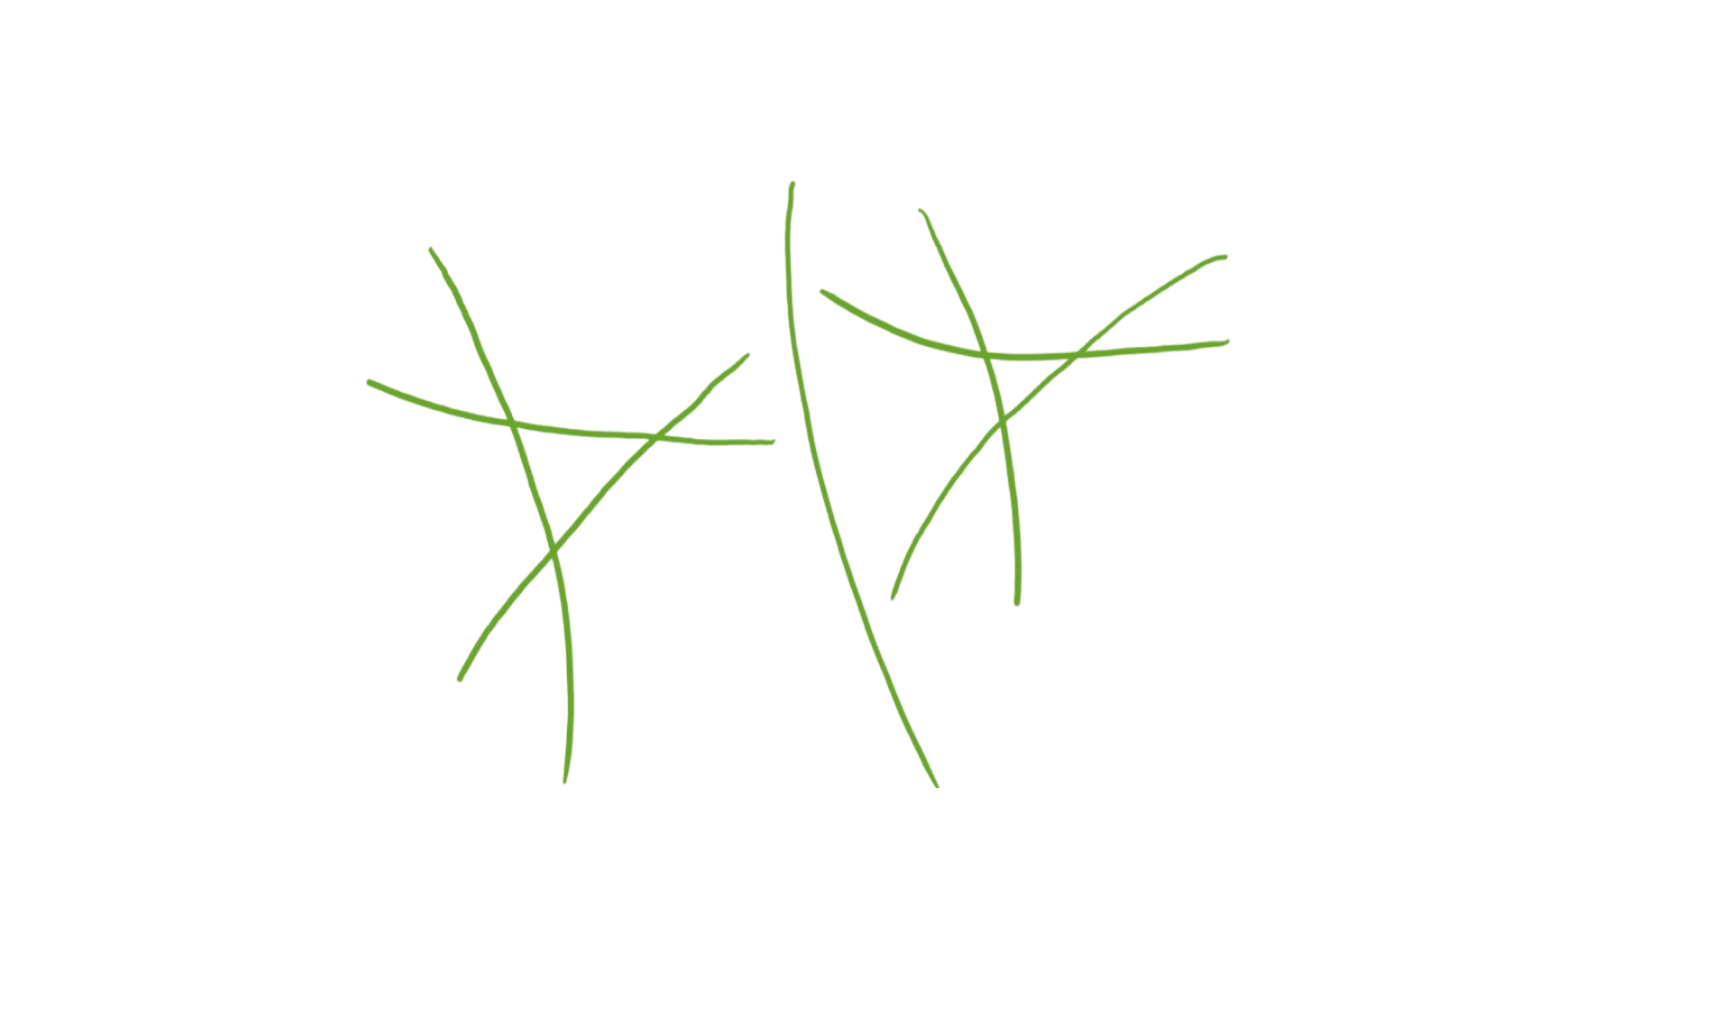
\includegraphics[width=0.9\textwidth]{img/plan/2_cuts.png}};}}
                \node[inner sep=0pt] at (5.5,-5) {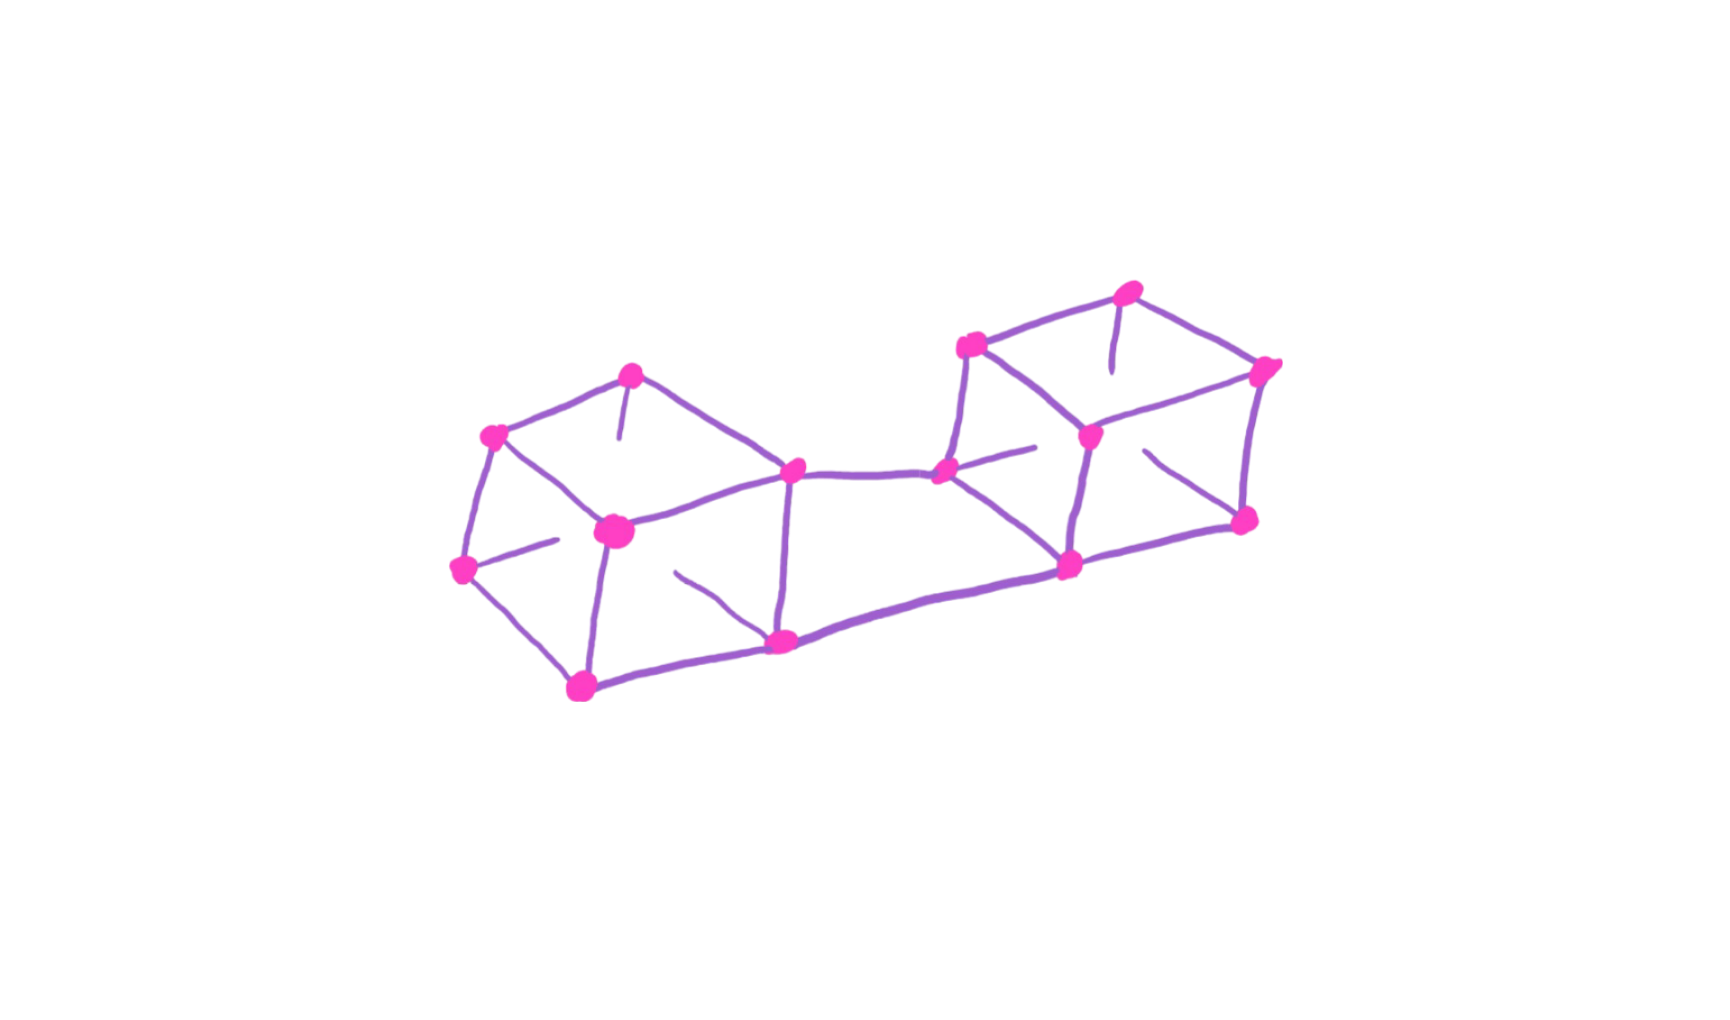
\includegraphics[width=0.83\textwidth]{img/plan/3_median.png}};
            \end{tikzpicture}
        }\end{center}

        \vspace{-0.4in}
        \pause

        \begin{theorem}[Sageev 95]
            If $\mc{H}$ is finitely-separating, then the graph $\mc{M}(\mc{H})$:
                \begin{itemize}
                    \item[\scriptsize$\blob$]\small Vertices are based orientations on $\mc{H}$;
                    \item[\scriptsize$\blob$]\small Neighbors of $U$ are $U\symdiff\l\{H,\lnot H\r\}$ for each minimal $H\in U\comp\l\{\lnot0\r\}$;
                \end{itemize}
            is a median graph.
        \end{theorem}
    \end{frame}
    \begin{frame}{Ends of graphs}
        \begin{definition}
            The \textit{end compactification} of a connected locally-finite $(X,G)$ is the Stone space $\widehat{X}$ of the Boolean algebra $\mc{H}_{\del<\infty}(X)$, whose non-principal ultrafilters are the \textit{ends} of $(X,G)$.
        \end{definition}

        \vspace{-0.2in}

        \only<1>{\begin{figure}[h]
            \center
            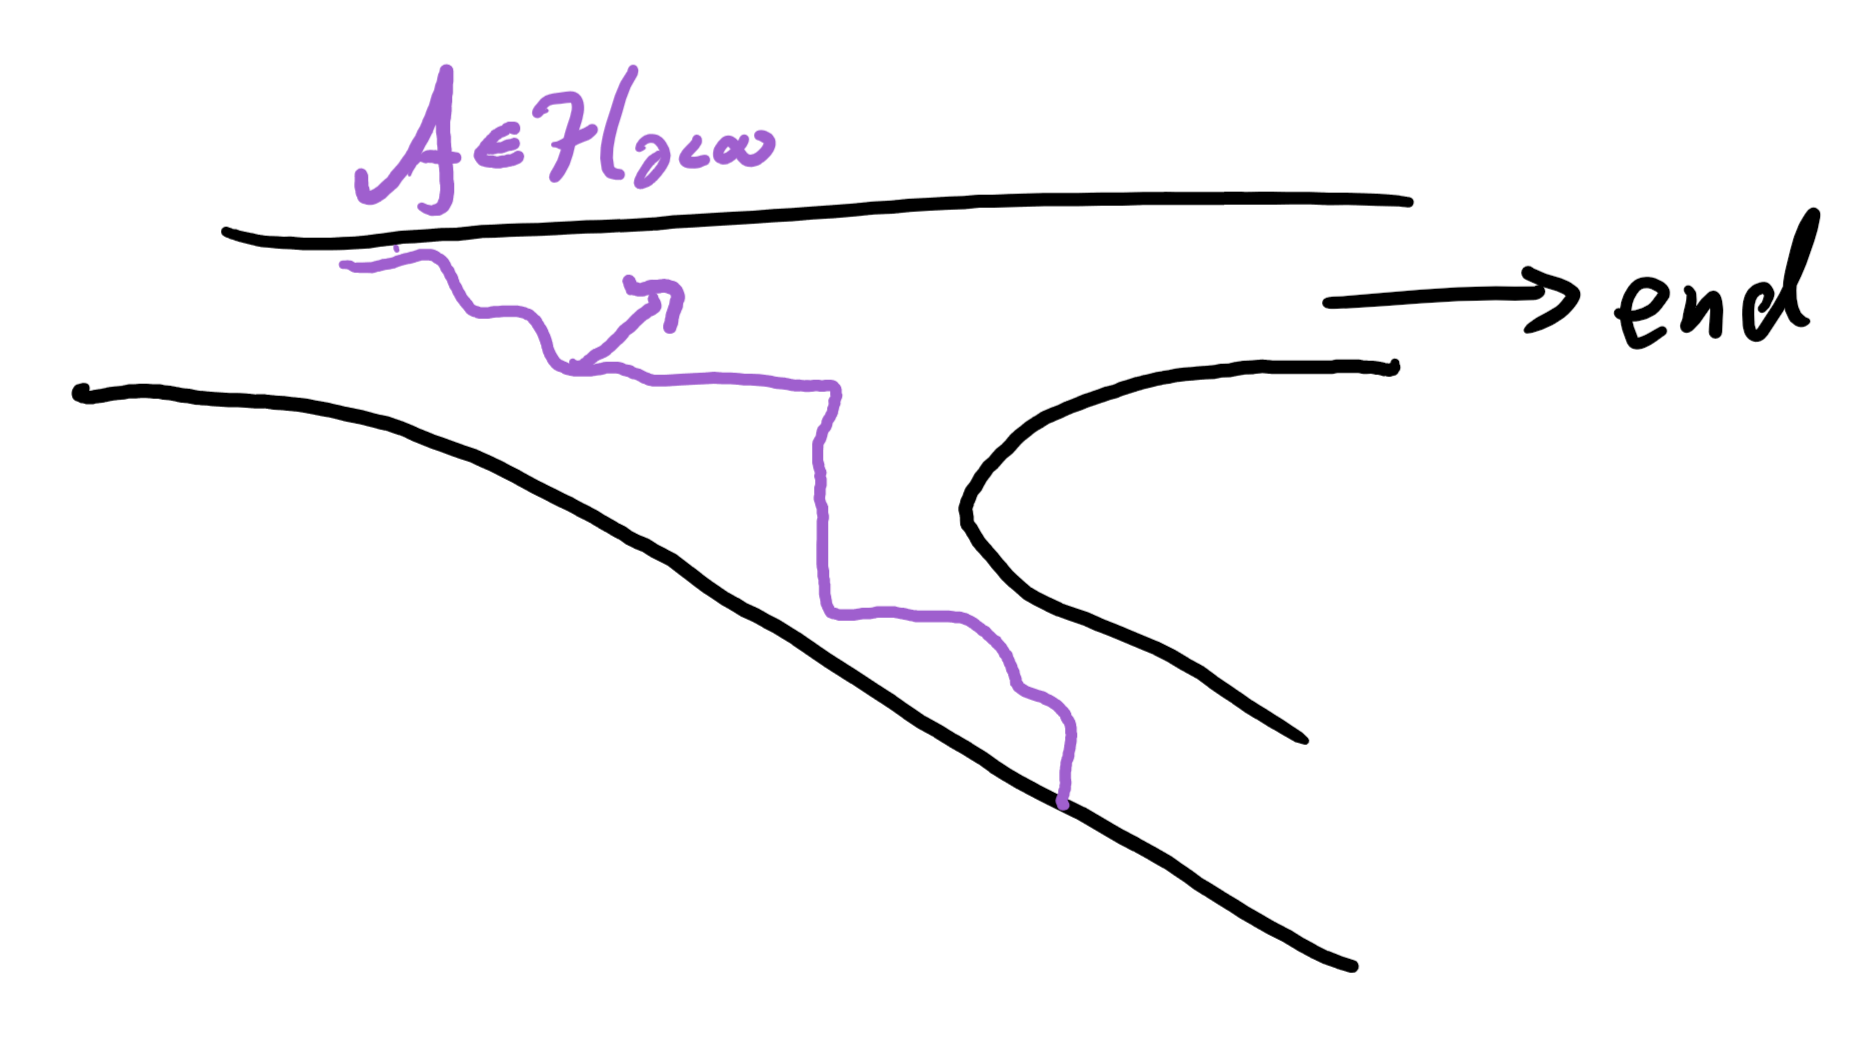
\includegraphics[width=0.6\textwidth]{img/end.png}
        \end{figure}}
        \only<2>{\begin{figure}[h]
            \center
            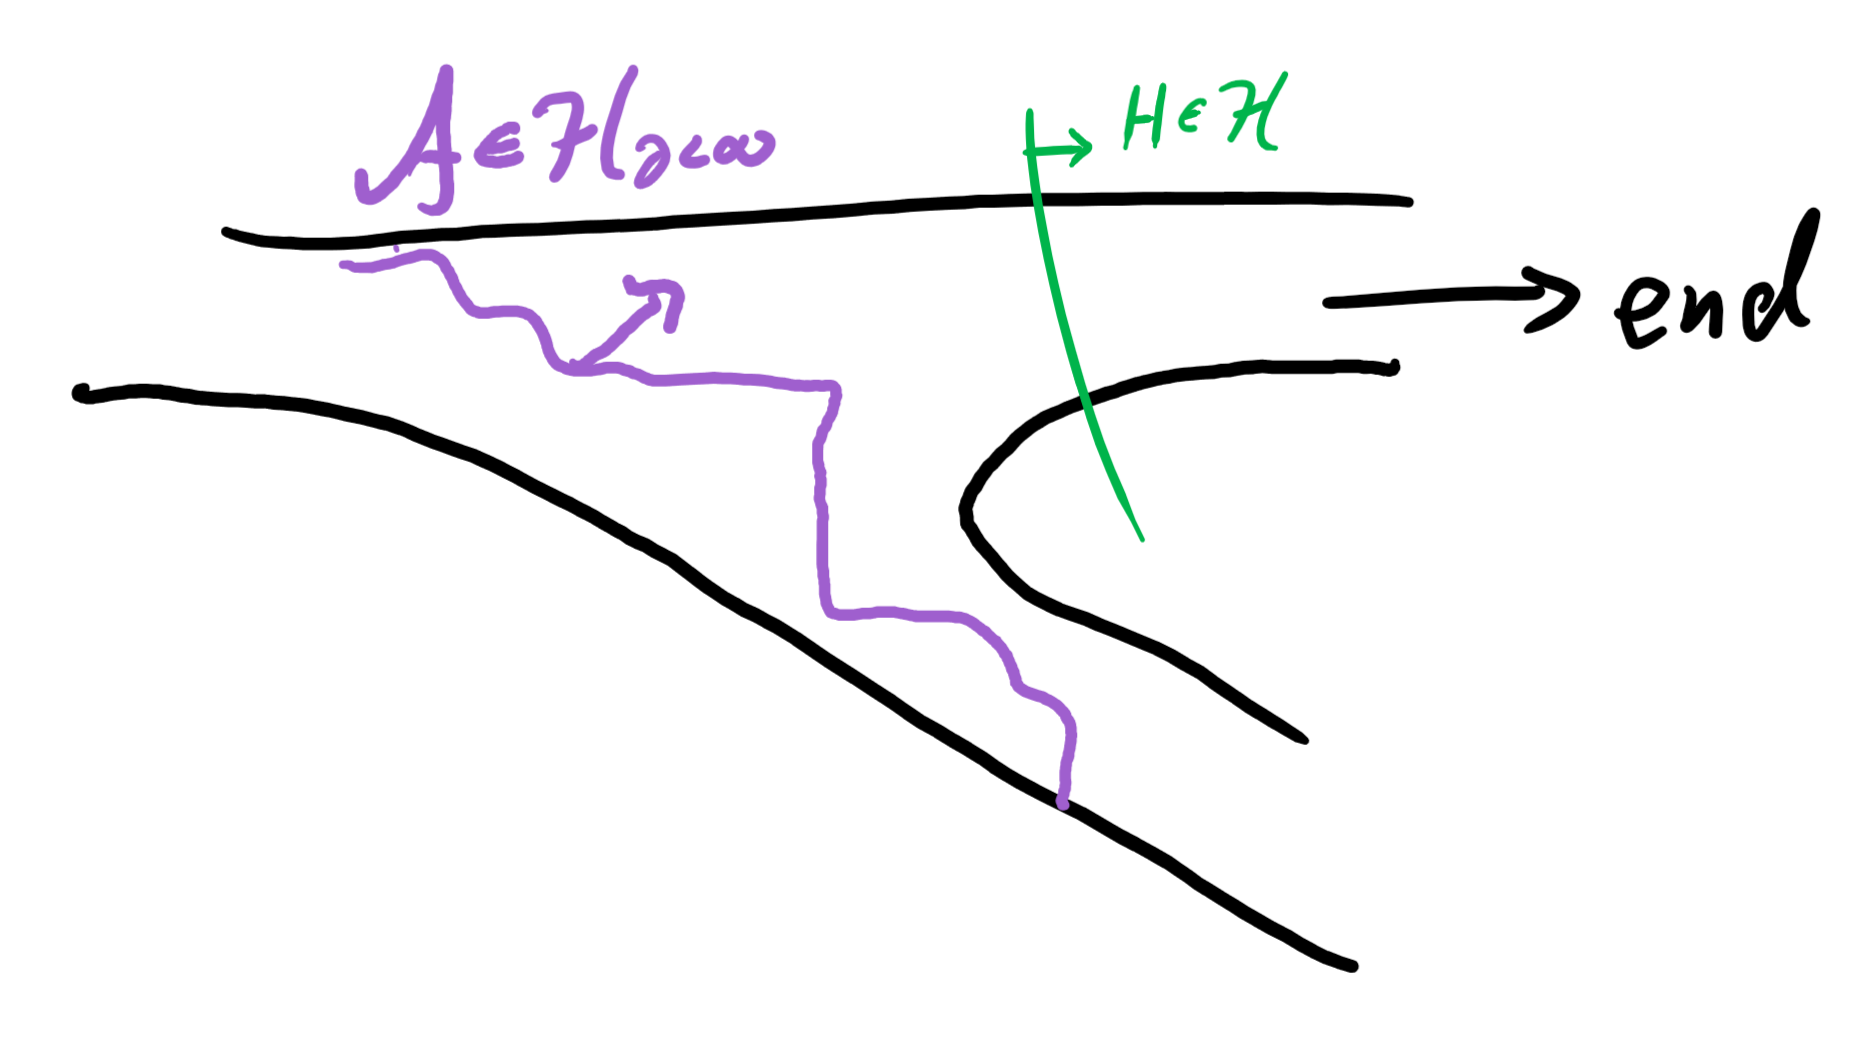
\includegraphics[width=0.6\textwidth]{img/dense_toward_end.png}
        \end{figure}}

        \pause
        \vspace{-0.2in}

        \begin{definition}
            A family $\mc{H}$ of cuts is \textit{dense towards ends} of $X$ if $\mc{H}$ contains a neighborhood basis for every end in $\widehat{X}$.
        \end{definition}
    \end{frame}
    \begin{frame}{Density towards ends for quasi-trees}
        \small{
            \begin{lemma}
                The connected locally-finite graphs in which $\mc{H}_{\diam(\del)\leq R}$ is dense towards ends for some $R<\infty$ is invariant under quasi-isometry.
            \end{lemma}

            \vspace{-0.1in}

            \begin{corollary}
                If $(X,G)$ is a locally-finite quasi-tree, then the family
                \vspace{-0.1in}
                \begin{equation*}
                    \mc{H}\coloneqq\mc{H}_{\diam(\del)\leq R}(X)\cap\mc{H}_{\mathrm{conn}}(X)
                    \vspace{-0.1in}
                \end{equation*}
                of cuts is dense towards ends for some $R<\infty$.
            \end{corollary}
            
            \vspace{-0.175in}

            \begin{figure}[h]
                \center
                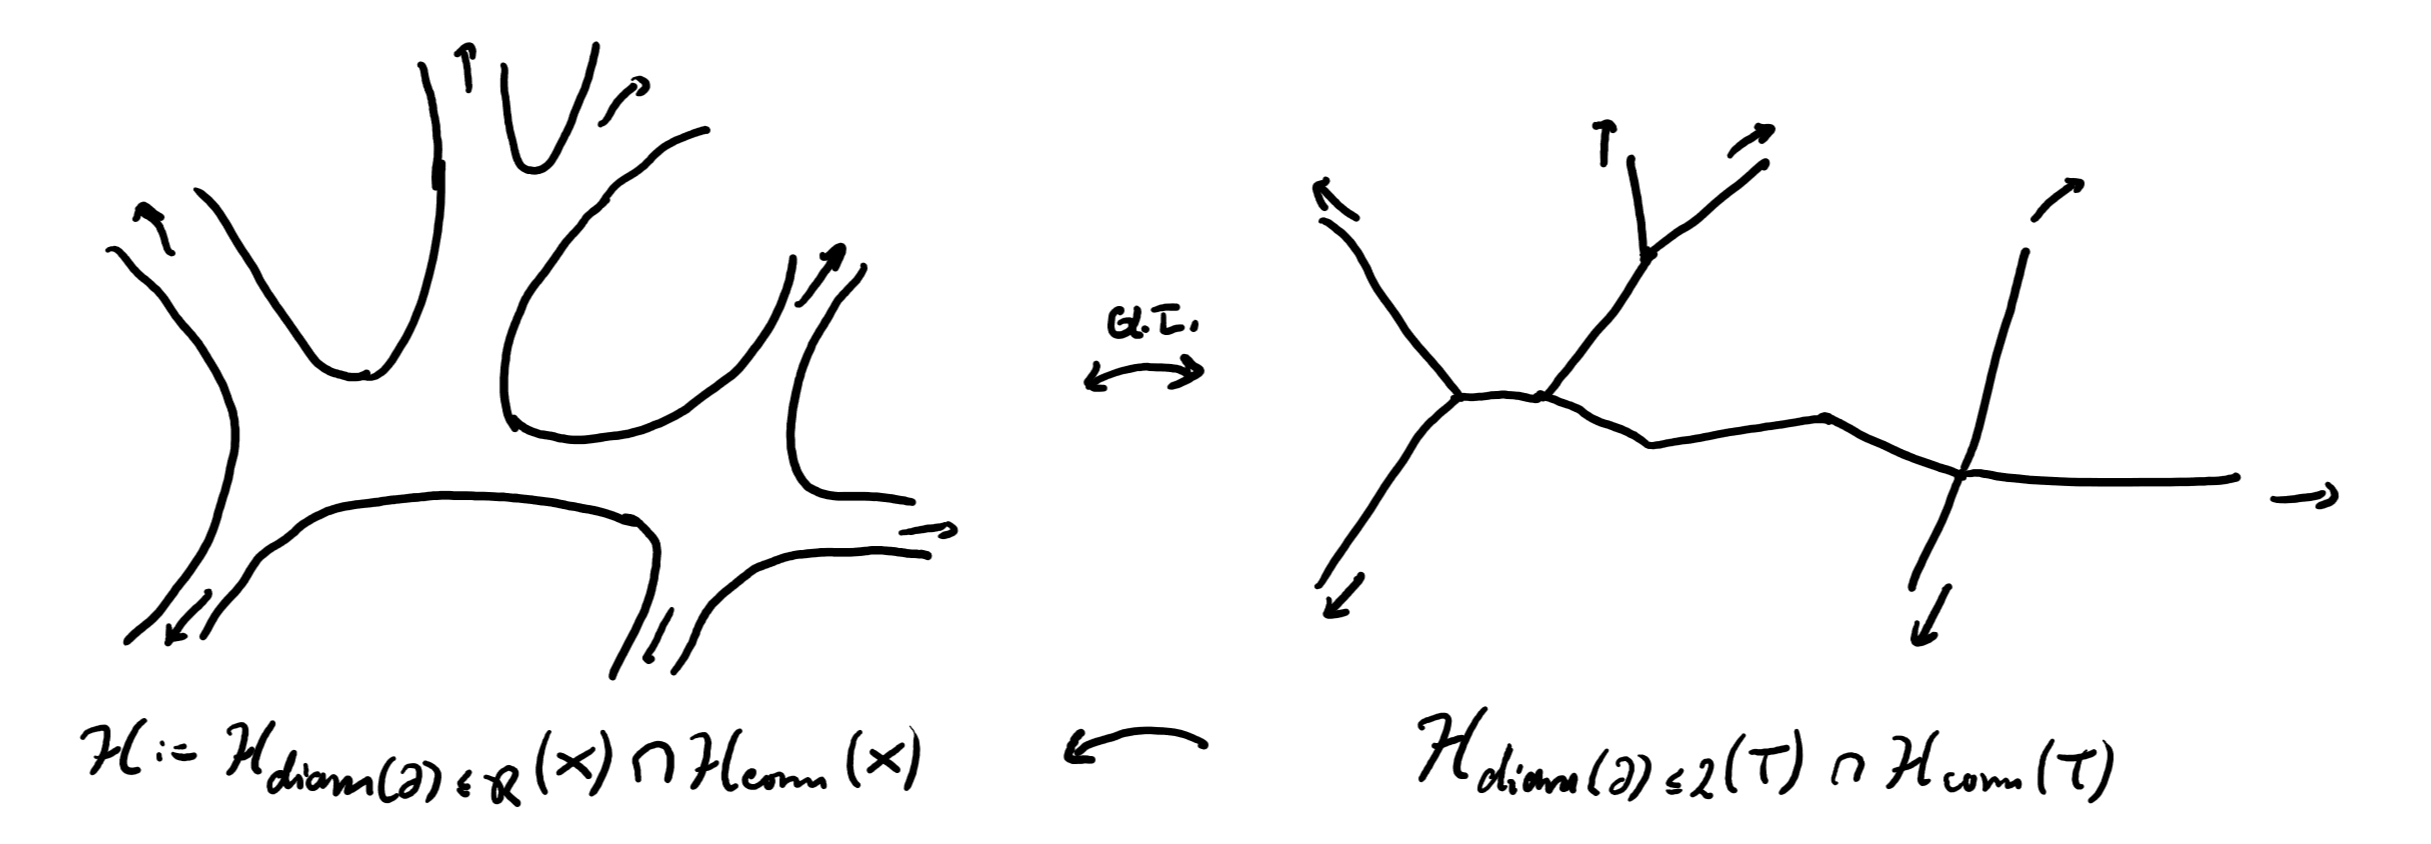
\includegraphics[width=0.8\textwidth]{img/tree_quasi_tree.png}
            \end{figure}
        }
    \end{frame}
    \begin{frame}{Wrapping things up...}
         \begin{center}
            \scalebox{0.85}{
                \hspace*{-0.62in}
                \def\hsp{3.75}
                \def\vsp{1.3}
                \def\vsh{0.05}
                \begin{tikzpicture}
                    \draw[dashed, rounded corners, opacity=0.2] (-1.7,0.5) -- (-1.7,-0.4-\vsp) -- (0.75,-0.4-\vsp) -- (3,-0.4) -- (3*\hsp+1.5,-0.4) -- (3*\hsp+1.5,0.5) -- cycle;
                    \draw[dashed, rounded corners, opacity=0.2] (2.5,0.55-\vsp) rectangle (3*\hsp+1.5,-0.45-\vsp);
                    \draw (0,\vsh) circle (0in) node{Quasi-treeing};
                    \draw (3*\hsp,\vsh) circle (0in) node{Treeing};
                    \draw[->] (0,-0.2) -- (0,-\vsp+0.3);
                    \draw (0,\vsh-\vsp) circle (0in) node{Quasi-tree};
                    \draw (\hsp,-\vsp) circle (0in) node{$\begin{gathered} \textrm{Finitely-sep.}\\[-4pt] \textrm{family of cuts} \end{gathered}$};
                    \draw[->] (1,\vsh-\vsp) -- (\hsp-1.1,\vsh-\vsp);
                    \draw (2*\hsp,-\vsp) circle (0in) node{$\begin{gathered} \textrm{Median graph w/}\\[-4pt] \textrm{finite hyperplanes} \end{gathered}$};
                    \draw[->] (\hsp+1.1,\vsh-\vsp) -- (2*\hsp-1.5,\vsh-\vsp);
                    \draw (3*\hsp,-\vsp) circle (0in) node{$\begin{gathered} \textrm{`Canonical'}\\[-4pt] \textrm{spanning tree} \end{gathered}$};
                    \draw[->] (2*\hsp+1.5,\vsh-\vsp) -- (3*\hsp-1.1,\vsh-\vsp);
                    \draw (\hsp,0) circle (0in) node{$\begin{gathered} \textrm{Dense family}\\[-4pt] \textrm{of cuts} \end{gathered}$};
                    \draw[->] (1,-1) -- (\hsp-1.1,0);
                    \draw[->] (\hsp+1.1,\vsh) -- (3*\hsp-1.1,\vsh);
                    \draw[->] (3*\hsp,0.4-\vsp) -- (3*\hsp,-0.2);
                    \draw (\hsp+1.1,-1) to [out=35, in=180] (2*\hsp,\vsh);

                    {\transparent{0.2}\node[inner sep=0pt] at (5,-5) {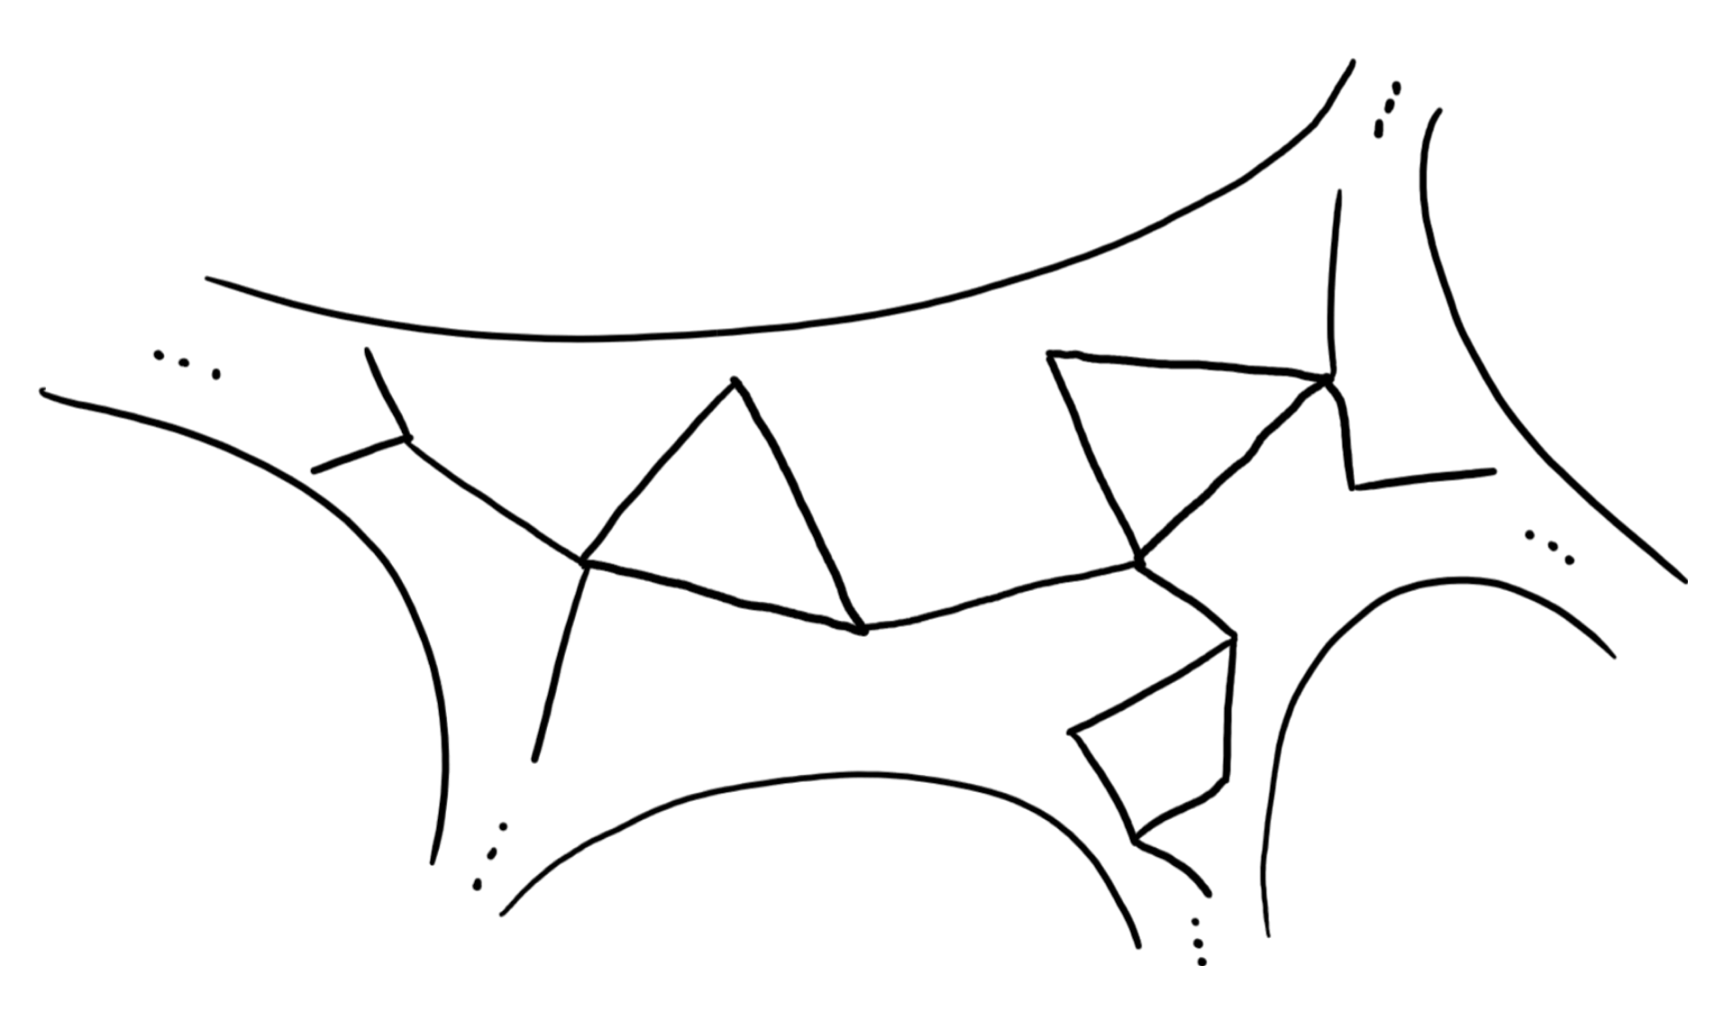
\includegraphics[width=0.9\textwidth]{img/plan/0_base.png}};}
                    {\transparent{0.3}\node[inner sep=0pt] at (5.8,-5.35) {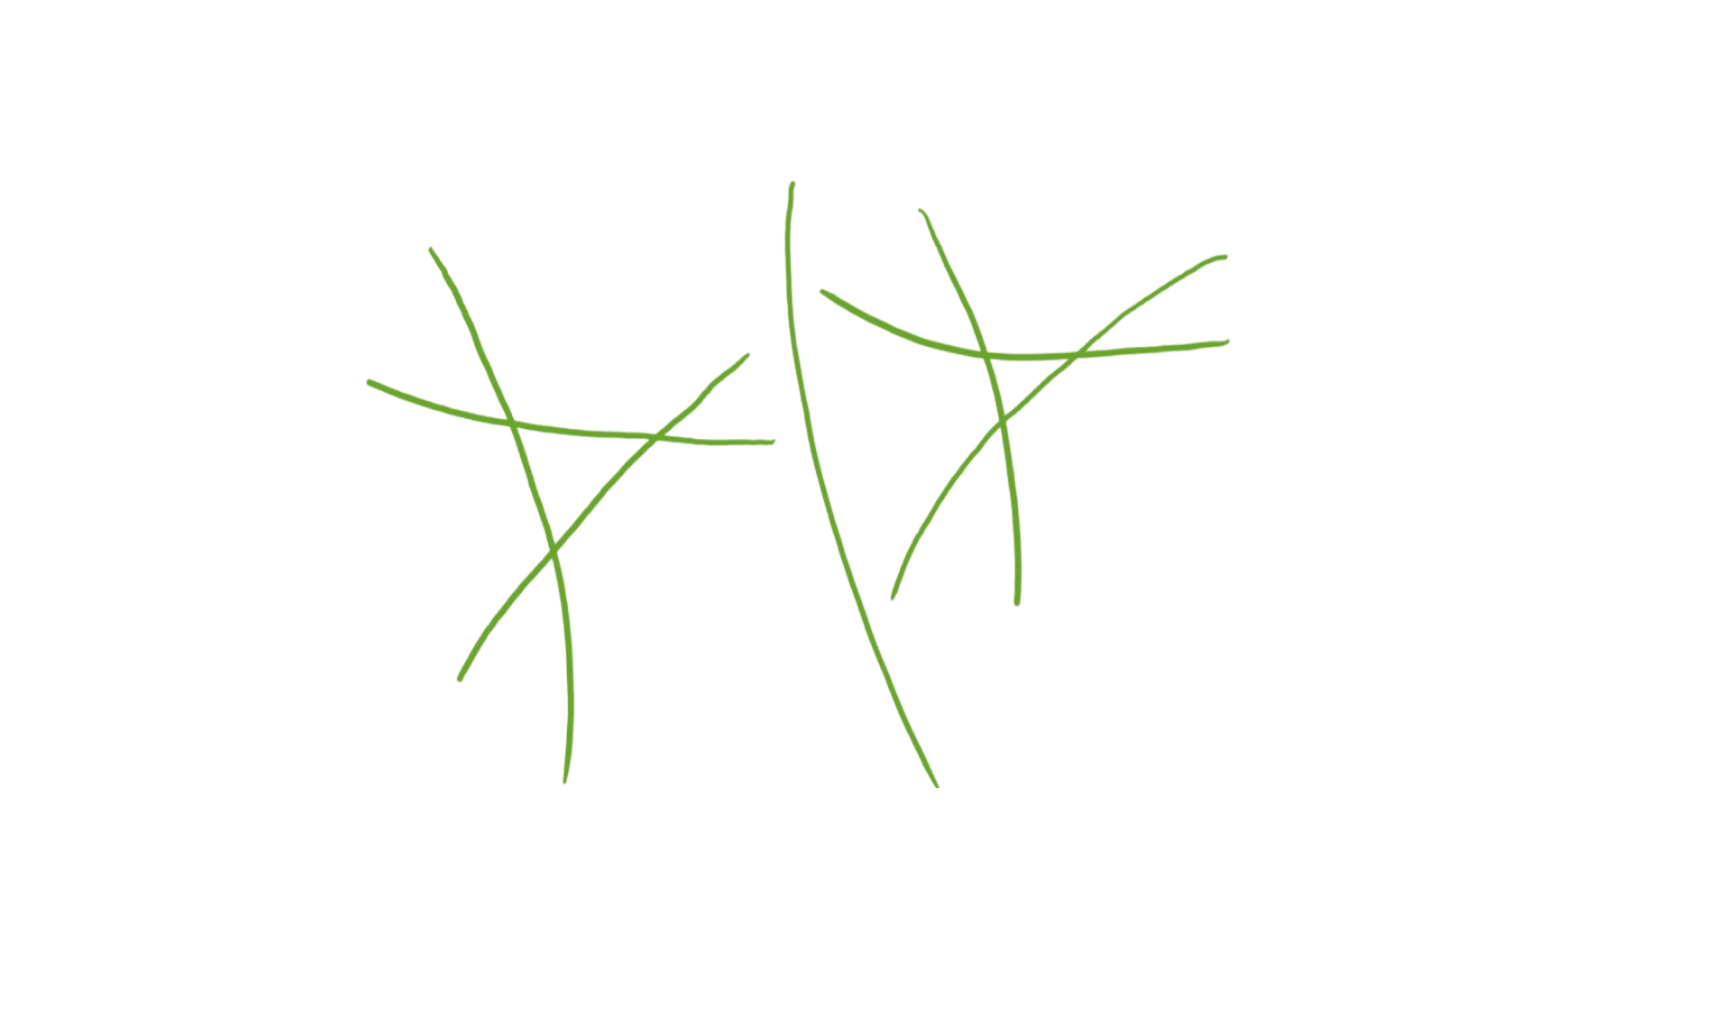
\includegraphics[width=0.9\textwidth]{img/plan/2_cuts.png}};}
                    {\transparent{0.6}\node[inner sep=0pt] at (5.5,-5) {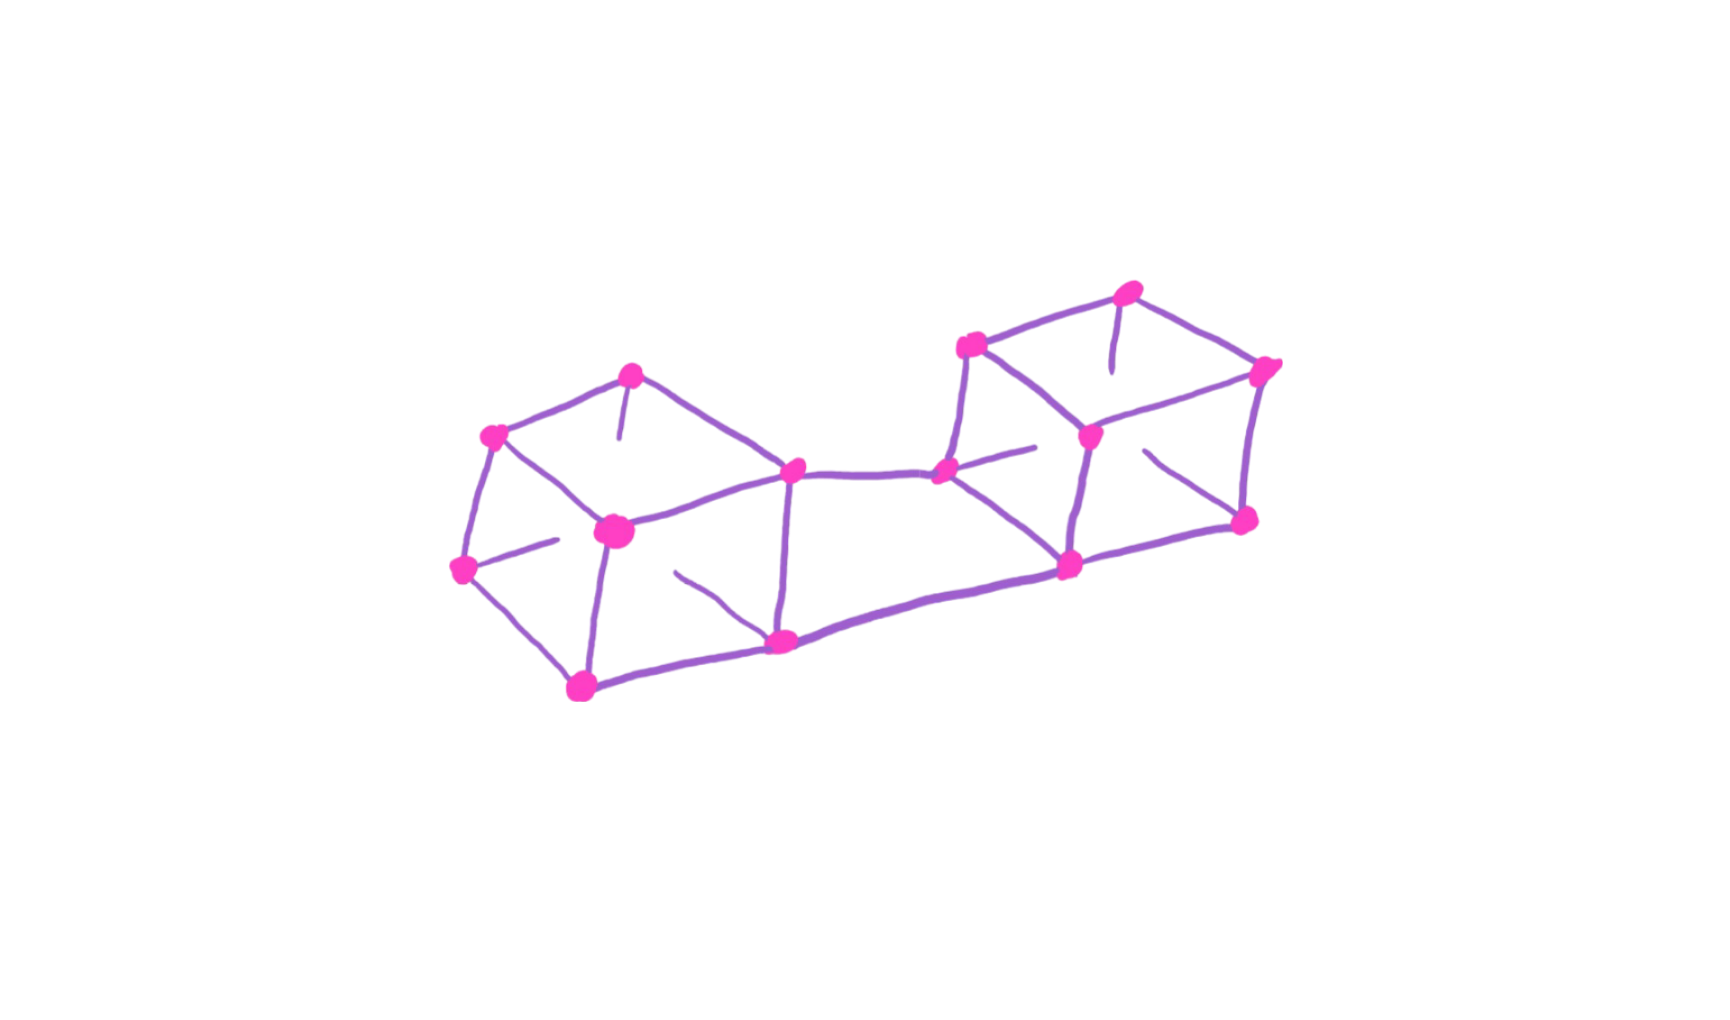
\includegraphics[width=0.83\textwidth]{img/plan/3_median.png}};}
                    \node[inner sep=0pt] at (5.76,-4.65) {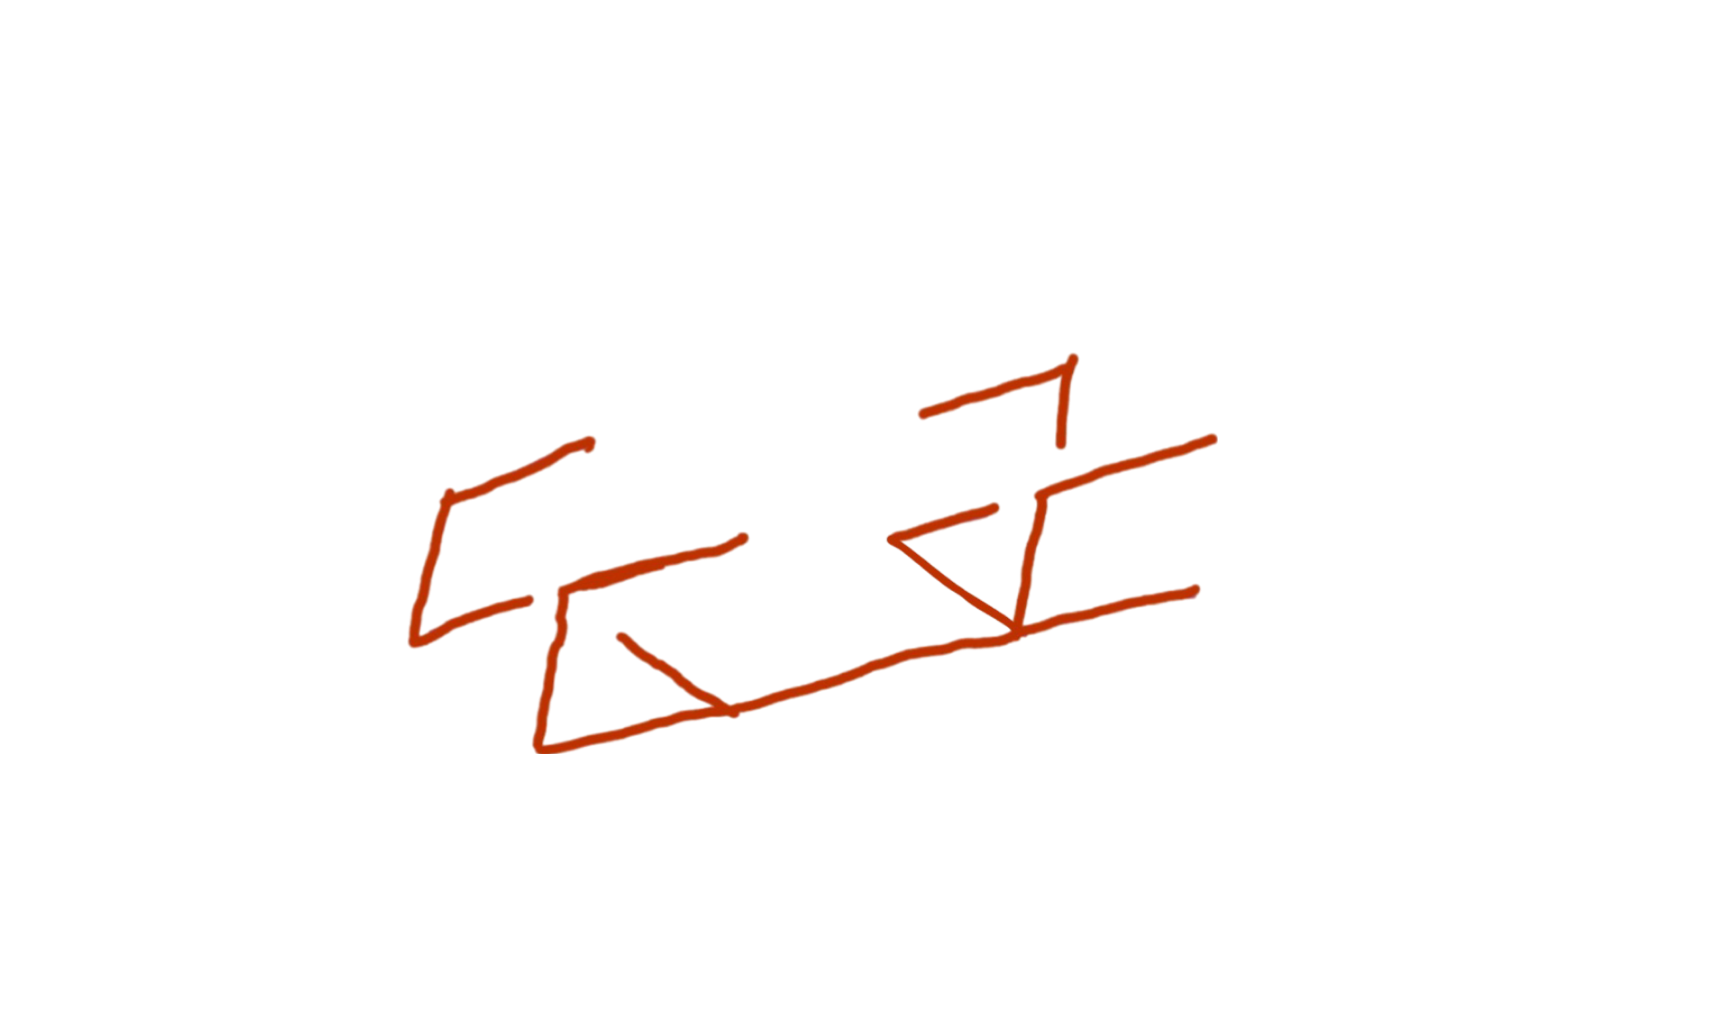
\includegraphics[width=0.83\textwidth]{img/plan/4_tree.png}};
                    {\transparent{0.3}\node[inner sep=0pt] at (5.1,-5.2) {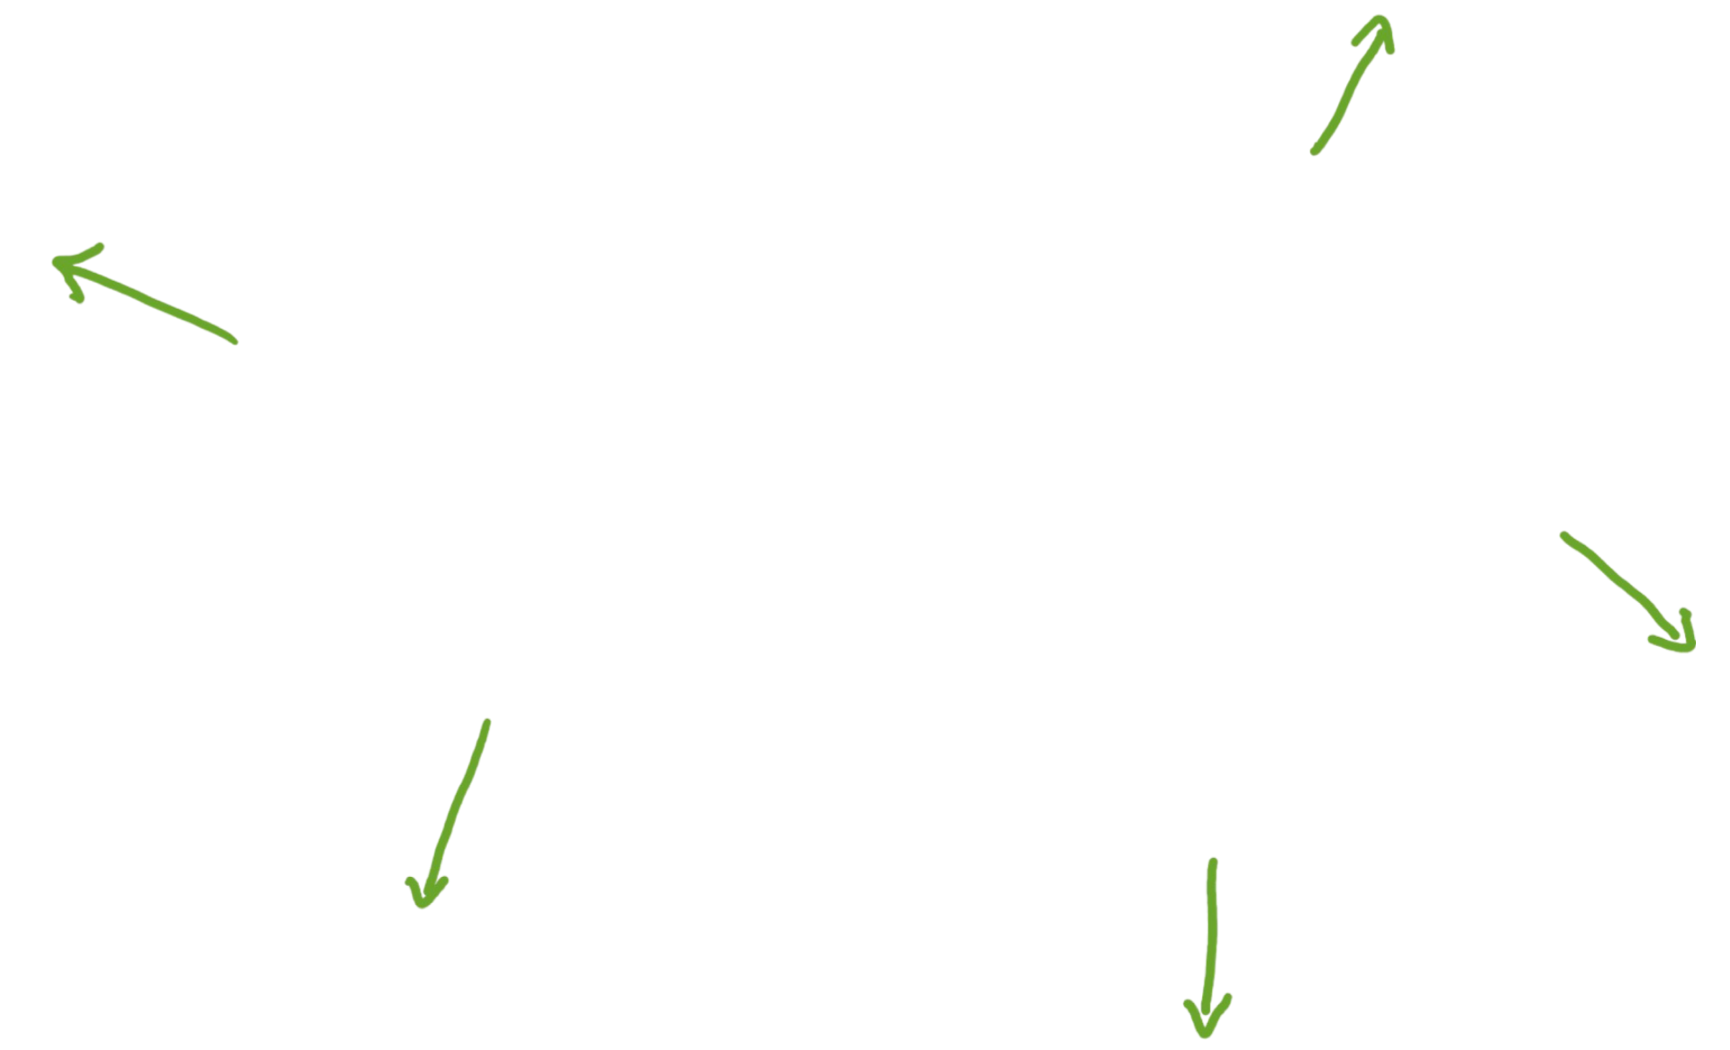
\includegraphics[width=0.9\textwidth]{img/plan/5_ends.png}};}
                \end{tikzpicture}
            }
        \end{center}
    \end{frame}
    \begin{frame}{The End}
        \begin{center}
            Thank you!
        \end{center}
    \end{frame}
\end{document}
